\chapter{WIMPs and neutrinos}\label{chapter:nufloor}
\lhead{\emph{WIMPs and neutrinos}}

\section{Introduction}
\label{sec:nufloor_intro}

Significant increases in sensitivity are expected in direct detection experiments over the next few years as detector target masses are increased to the ton-scale and beyond. As anticipated in early work on direct detection, these large detectors will also be able to detect coherent scattering between astrophysical neutrinos and nuclei~\cite{Cabrera:1984rr,Monroe:2007xp,Strigari:2009bq,Gutlein:2010tq}. Neutrinos are therefore the ultimate background for WIMP direct detection searches as they cannot be shielded against and produce recoils with similar rates and energy spectra~\cite{Monroe:2007xp,Strigari:2009bq,Gutlein:2010tq,Billard:2013qya}.

For near-future direct detection experiments the most problematic types of neutrino are those produced in $^8$B decay in the Sun and in cosmic ray collisions in the Earth's atmosphere. In a xenon detector the recoil energy spectrum and rate from ${}^{8}\rm{B}$ neutrinos very closely matches that of a WIMP with mass $m_{\chi}= 6 \, {\rm GeV}$ and cross section $\sigma^{\rm SI}_p \sim 5 \times 10^{-45} \, {\rm cm}^2$, while the spectrum from atmospheric neutrinos is similar to that of a WIMP with $m_{\chi} \sim 100 \, {\rm GeV}$ and  $\sigma^{\rm SI}_p \sim  10^{-48} \, {\rm cm}^2$~\cite{Strigari:2009bq}. Consequently the sensitivity of an experiment to WIMPs reaches a point of saturation where it becomes difficult to tell the difference between WIMP and neutrino induced recoils using their energies alone. So as the exposure of an experiment increases the minimum discoverable cross section rather than decreasing reaches a plateau. The point at which this occurs depends on the systematic uncertainty in the neutrino flux and is commonly referred to as the ``neutrino floor''~\cite{Billard:2013qya}.

The neutrino floor is not however the true final limit to direct detection. As initially shown by Ruppin~\etal~\cite{Ruppin:2014bra}, the differences in the tails of the recoil energy distributions between WIMPs and neutrinos allow the ``floor'' to be overcome with high statistics (typically $>\mathcal{O}(1000)$ events). It has also been shown that for some of the additional operators posited in the non-relativistic effective field theory formalism the recoil spectra are sufficiently distinct from neutrinos to allow their discrimination with fewer events than in the standard SI or SD cases~\cite{Dent:2016iht,Dent:2016wor}. However, as we will explore further, the shape of the neutrino floor limit will necessarily be dependent on astrophysical uncertainties. Hence if an accurate prediction is to be made about when future experiments will be affected by the neutrino background at a statistically significant level, we must also establish the extent to which the uncertainty in the astrophysical input plays a role. In this Chapter we expand upon results from the literature by embedding these astrophysical uncertainties in the neutrino floor calculation.

If the detection of dark matter is not imminent and requires that we probe cross sections below the floor then it will be crucial to search for ways to distinguish the WIMP and neutrino signals, for instance via their different time or direction dependencies. The flux of Solar neutrinos is also annually modulated due to the eccentricity of the Earth's orbit. With very large exposures adding timing information allows the neutrino floor to be suppressed at low WIMP masses~\cite{Davis:2014ama}. The complementarity of the recoil spectra from multiple target nuclei can also be exploited to probe below the neutrino floor set by a single type of nucleus. This is a good tactic for SD interactions where there is much nucleus-to-nucleus difference in the expected scattering rates, but only marginally improves the discovery limit in the SI case~\cite{Ruppin:2014bra}. One would expect the most powerful technique to subtract the neutrino background to be directional detection. The unique directional signature of the WIMP event rate is in direct contrast with Solar neutrinos, which will point back towards the Sun, and atmospheric and supernovae neutrinos which are expected to be mostly isotropic. If a directional detector can be scaled up to a point at which it is sensitive to coherent neutrino-nucleus scattering then it will inherently set better limits than an equivalent non-directional experiment.

In the first Section we review each contribution to the neutrino background relevant for direct detection. We describe the resulting signals in both conventional and directional experiments. In Sec.~\ref{sec:nufloor_nufloor} we describe in detail the effect of the neutrino background on the discovery of dark matter, explaining the calculation and phenomenology of the neutrino floor and the impact of various sources of uncertainty. Then in the penultimate section of this Chapter, Sec.~\ref{sec:nufloor_time}, we explore ways of subtracting the neutrino background and circumventing the floor. We briefly comment upon the use of time dependence before focusing on directional detectors. We summarise and discuss future strategies in Sec.~\ref{sec:nufloor_conc}.

\section{The neutrino background}

\subsection{Fluxes}
\begin{figure}
\begin{center}
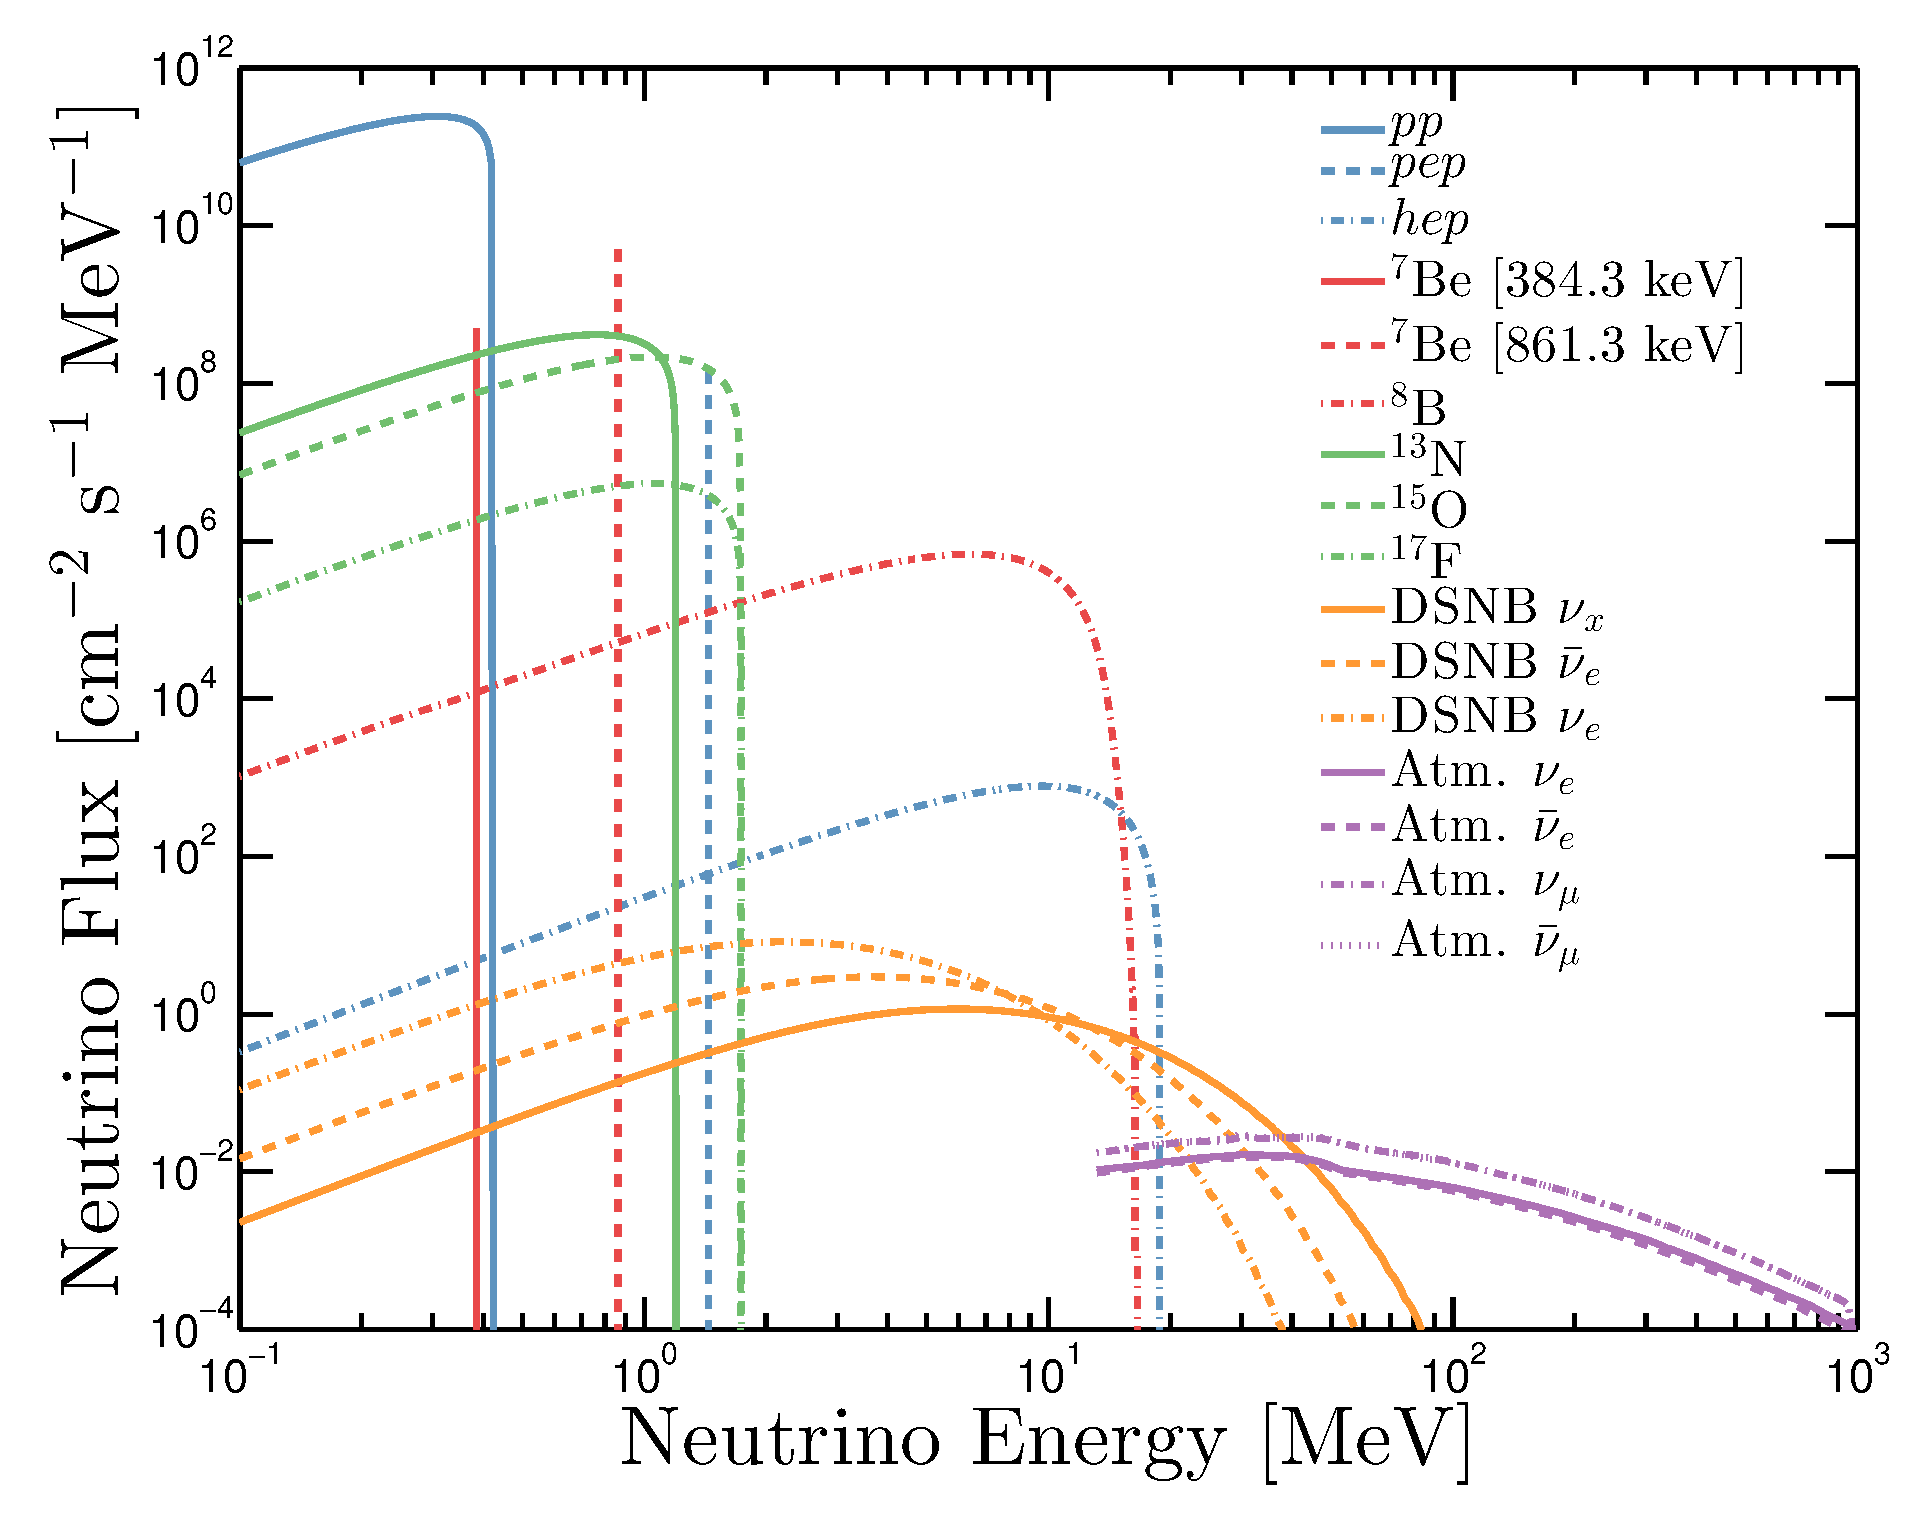
\includegraphics[trim = 5mm 0 0mm 3mm, clip, width=0.8\textwidth,angle=0]{Figures/neutrino_flux.eps}
\caption[Fluxes for neutrino backgrounds]{Neutrino energy spectra that are backgrounds to direct detection experiments: Solar, atmospheric, and the diffuse supernovae background (DSNB).} 
\label{fig:Flux}
\end{center}
\end{figure} 

\begin{table}[t]\centering
\ra{1.3}
\begin{tabularx}{\textwidth}{cc|cc|Y}
\hline\hline
$\mathbf{\nu}$ \bf{type} &  & $\mathbf{E_{\nu}^{\rm{max}}}$ \bf{(MeV)} & $\mathbf{E_{r_{\rm{Xe}}}^{\rm{max}}}$ \bf{(keV)} & $\Phi\pm \delta\Phi$ $\mathbf{(\rm{cm^{-2} \, s^{-1}})}$\\
\hline
\multirow{8}{*}{\bf Solar} &$pp$ & 0.42341 & $2.94\times 10^{-3}$ & $\left(5.98\pm 0.036 \right) \times 10^{10}$\\
&${}^{7}\rm{Be}$ & 0.8613 & 0.0122 & $\left( 5.00\pm 0.35 \right) \times 10^9$\\
&$pep$ & 1.440 & 0.0340 & $\left( 1.44\pm 0.017\right) \times 10^8$\\
&${}^{13}\rm{N}$ & 1.199 & 0.02356 & $\left(2.96\pm 0.41\right) \times 10^8 $\\
&${}^{15}\rm{O}$ & 1.732 & 0.04917 & $\left(2.23\pm 0.34\right) \times 10^8$\\
&${}^{17}\rm{F}$ & 1.740 & 0.04962 & $\left(5.52\pm 0.94 \right) \times 10^6$\\
&${}^{8}\rm{B}$ & 16.360 & 4.494 & $\left(5.16\pm 0.11\right) \times 10^6$\\
&$hep$ & 18.784 & 5.7817 & $\left( 8.04\pm 2.41 \right) \times 10^3$\\
\hline
\multirow{3}{*}{\bf DSNB}&$\nu_e$  &  &  & \\
&$+\bar{\nu}_e$  & $>$91.201 & $>$136.1 & $ 85.7\pm 42.7$\\
&$+\nu_x$  &  & & \\
\hline
\multirow{4}{*}{{\bf Atm.}}& $\nu_e$ & \multirow{4}{*}{$>$981.748} & \multirow{4}{*}{$>15.55\times 10^3$} & \multirow{4}{*}{$10.54\pm 2.1$}\\
&$+\bar{\nu}_e$ & &  &\\
&$+\nu_\mu$ &  &  &\\
&$+\bar{\nu}_\mu$ &  & & \\
\hline \hline
\end{tabularx}
\caption[Total neutrino fluxes with corresponding uncertainties]{Total neutrino fluxes with corresponding uncertainties. All solar neutrino fluxes are from the updated high metallicity SSM (Ref.~\cite{Serenelli:2011py}) with the exception of $^8$B which is from an analysis of neutrino data (Ref.~\cite{Bergstrom:2016cbh}). The DSNB and atmospheric neutrino fluxes are from Refs.~\cite{Beacom:2010kk} and~\cite{Honda:2011nf} respectively. The maximum neutrino energy, $E_{\nu}^{\rm{max}}$, and maximum recoil energy for a xenon target, $E_{r_{\rm{Xe}}}^{\rm{max}}$, are also shown. For atmospheric neutrinos and the DSNB we indicate the maximum neutrino energy used, though these fluxes in principle extend to higher energies.\label{tab:neutrino}}
\end{table}


To begin we describe the Solar, atmospheric and diffuse supernovae background neutrinos (DSNB) which scatter with nuclei into energies relevant for direct detection experiments. We expand upon previous results in the literature by highlighting the angular dependence of these fluxes. We display the energy spectra for each source of neutrino in Fig.~\ref{fig:Flux} and list each flux normalisation, $\Phi$, and uncertainty, $\delta \Phi$, in Table~\ref{tab:neutrino}.

{\bf Solar neutrinos} from nuclear fusion reactions in the interior of the Sun dominate the low energy-high flux regime and are the major neutrino background for direct detection with a total flux at Earth of $6.5\times10^{11}$~cm$^{-2}$~s$^{-1}$~\cite{Robertson:2012ib,Antonelli:2012qu}. Neutrinos from the initial proton-proton fusion reaction ``$pp$'' make up 86\% of the Solar emission and have been detected most recently by the Borexino experiment, which determined the flux with an uncertainty of $\sim 10$\% ~\cite{Bellini:2014uqa}. Despite the huge flux of $pp$ neutrinos they yield nuclear recoil energies well below the threshold of any direct detection experiment\footnote{$pp$ neutrinos would however be the dominant source of electron recoils.}. Secondary fusion of $p+e^-+p$ and $^3 $He$~+~p$ produce neutrinos, labelled ``$pep$'' and ``$hep$'', extend to energies beyond $pp$ neutrinos but with much lower flux. Shown in Fig.~\ref{fig:Flux} as lines are the two fluxes of monoenergetic neutrinos associated with $^7$Be electron capture. The lines have energies of 384.3~keV and 861.3~keV with branching ratios of $\sim$10\% and $\sim$90\% respectively. The latter of these is principally responsible for limiting the discovery for $m_\chi<1$~GeV so may become important in future ultra-low threshold light WIMP searches~\cite{Strigari:2016ztv}. In the following we ignore the Doppler broadening of these lines, as well as the $pep$ line, which would induce a negligible correction to the subsequent recoil energy spectrum. Next we have neutrinos due to the decay of $^8$B which extend up to $\sim$10 MeV in energy placing them within the reach of dark matter searches. The spectrum of $^8$B neutrinos mimics the signal from a WIMP with a mass of 6~GeV and will likely be the first to be detected (via nuclear recoils) in future direct detection experiments. Finally we have neutrinos arising from the carbon-nitrogen-oxygen (CNO) cycle labelled by the decay from which they originate: $^{13}$N, $^{15}$O and $^{17}$F. These are at present unmeasured but Borexino places an upper bound of $<7.7\times10^8$~cm$^{-2}$~s$^{-1}$ on the sum of their flux~\cite{Bellini:2013lnn}. CNO neutrinos are a subdominant background for us but are of great interest to studies of stellar physics since their flux is highly sensitive to the Solar metallicity. 

The theoretical systematic uncertainties on the Solar neutrino fluxes range from 1\% ($pp$ flux) to 14\% ($^8$B flux). Although out of these various components, four have now been directly measured: $pp$, $pep$, $^8$B and $^7$Be. For all except $^8$B, the theoretical uncertainty is smaller than the measurement uncertainty. The theoretical uncertainty arises largely from the uncertainty in the Solar metallicity, and in order to establish a self-consistent model of Solar neutrino fluxes one must assume a metallicity model. The Standard Solar models (SSMs) of Grevesse \& Sauval~\cite{Grevesse:1998bj} are broadly split into two categories `high-Z' and `low-Z' based on the assumed Solar metallicity,~Z. Both models have historically disagreed with some set of observables such as neutrino data, helioseismology or surface helium abundance~\cite{Villante:2013mba}. To remain consistent with previous neutrino floor calculations (e.g. Ref.~\cite{Ruppin:2014bra}) we consider the high-Z model. We use values presented in Ref.~\cite{Serenelli:2011py} which are based on updated fusion cross sections~\cite{Adelberger:2010qa}. The most recent generation of SSMs from Vinyoles~\etal~\cite{Vinyoles:2016djt} have a mild preference towards a high-Z configuration, though the authors note that neither are free from some level of disagreement with the various Solar observables\footnote{Dark matter detection experiments may shed further light on the Solar metallicity issue, e.g. Refs.~\cite{Billard:2014yka,Strigari:2016ztv,Cerdeno:2016sfi}. The measurement of CNO neutrinos will be essential for this, and may be possible in the future for instance with a neon target experiment as suggested by Ref.~\cite{Cerdeno:2016sfi}.}. We set our systematic uncertainties on each flux to the theoretical estimate with the exception of $\delta \Phi_{^8{\rm B}}$ for which the measurement uncertainty is smaller; we use the result presented in Ref.~\cite{Bergstrom:2016cbh} based on a global analysis of all Solar and terrestrial neutrino data. 

In addition to the spectra and flux of Solar neutrinos, we are also interested in their direction and time dependence. Due to the eccentricity of the Earth's orbit, the Earth-Sun distance has an annual variation leading to a modulation in the Solar neutrino flux as seen by an Earth-based experiment such that,
\begin{equation}
  \frac{\textrm{d}^2 \Phi(t)}{\textrm{d}E_\nu \textrm{d}\Omega_\nu}  =  \frac{\textrm{d} \Phi}{\textrm{d} E_\nu} \,\left[ 1 + 2 e \cos\left(\frac{2\pi(t- t_\nu)}{T_\nu}\right) \right] 
 \delta\left(\hat{{\bf q}}_\nu-\hat{{\bf q}}_\odot(t)\right) \,,
\label{eq:solarneutrinoflux_directional}
\end{equation}
where $t$ is the time from January 1st, $e = 0.016722$ is the eccentricity of the Earth's orbit, $t_{\nu} = 3$ days is the time at which the Earth-Sun distance is minimum (and hence the Solar neutrino flux is largest), $T_{\nu} = 1$ year, $\hat{{\bf q}}_{\nu}$ is a unit vector in the direction of interest and $\hat{{\bf q}}_\odot(t)$ is a unit vector in the inverse of the direction towards the Sun\footnote{We ignore the angular size of the Sun's core on the sky which would cause a tiny angular spread in the incoming neutrino directions, see e.g. Ref.~\cite{Davis:2016hil}.}. This annual modulation has been observed most recently in $^7$Be neutrinos by Borexino~\cite{Agostini:2017iiq}.


{\bf Atmospheric neutrinos} due to cosmic ray collisions are responsible for the neutrino floor for WIMP masses around $\sim$100 GeV and will limit the discovery of SI cross sections below approximately $10^{-48}$ cm$^2$~\cite{Strigari:2009bq,Billard:2013qya,Ruppin:2014bra}. The flux of atmospheric neutrinos at the relevant low energies ($\sim$100 MeV) is difficult to both measure and theoretically predict~\cite{Battistoni:2005pd} so currently has uncertainties of around 20\%~\cite{Honda:2011nf}.

\begin{figure}
\begin{center}
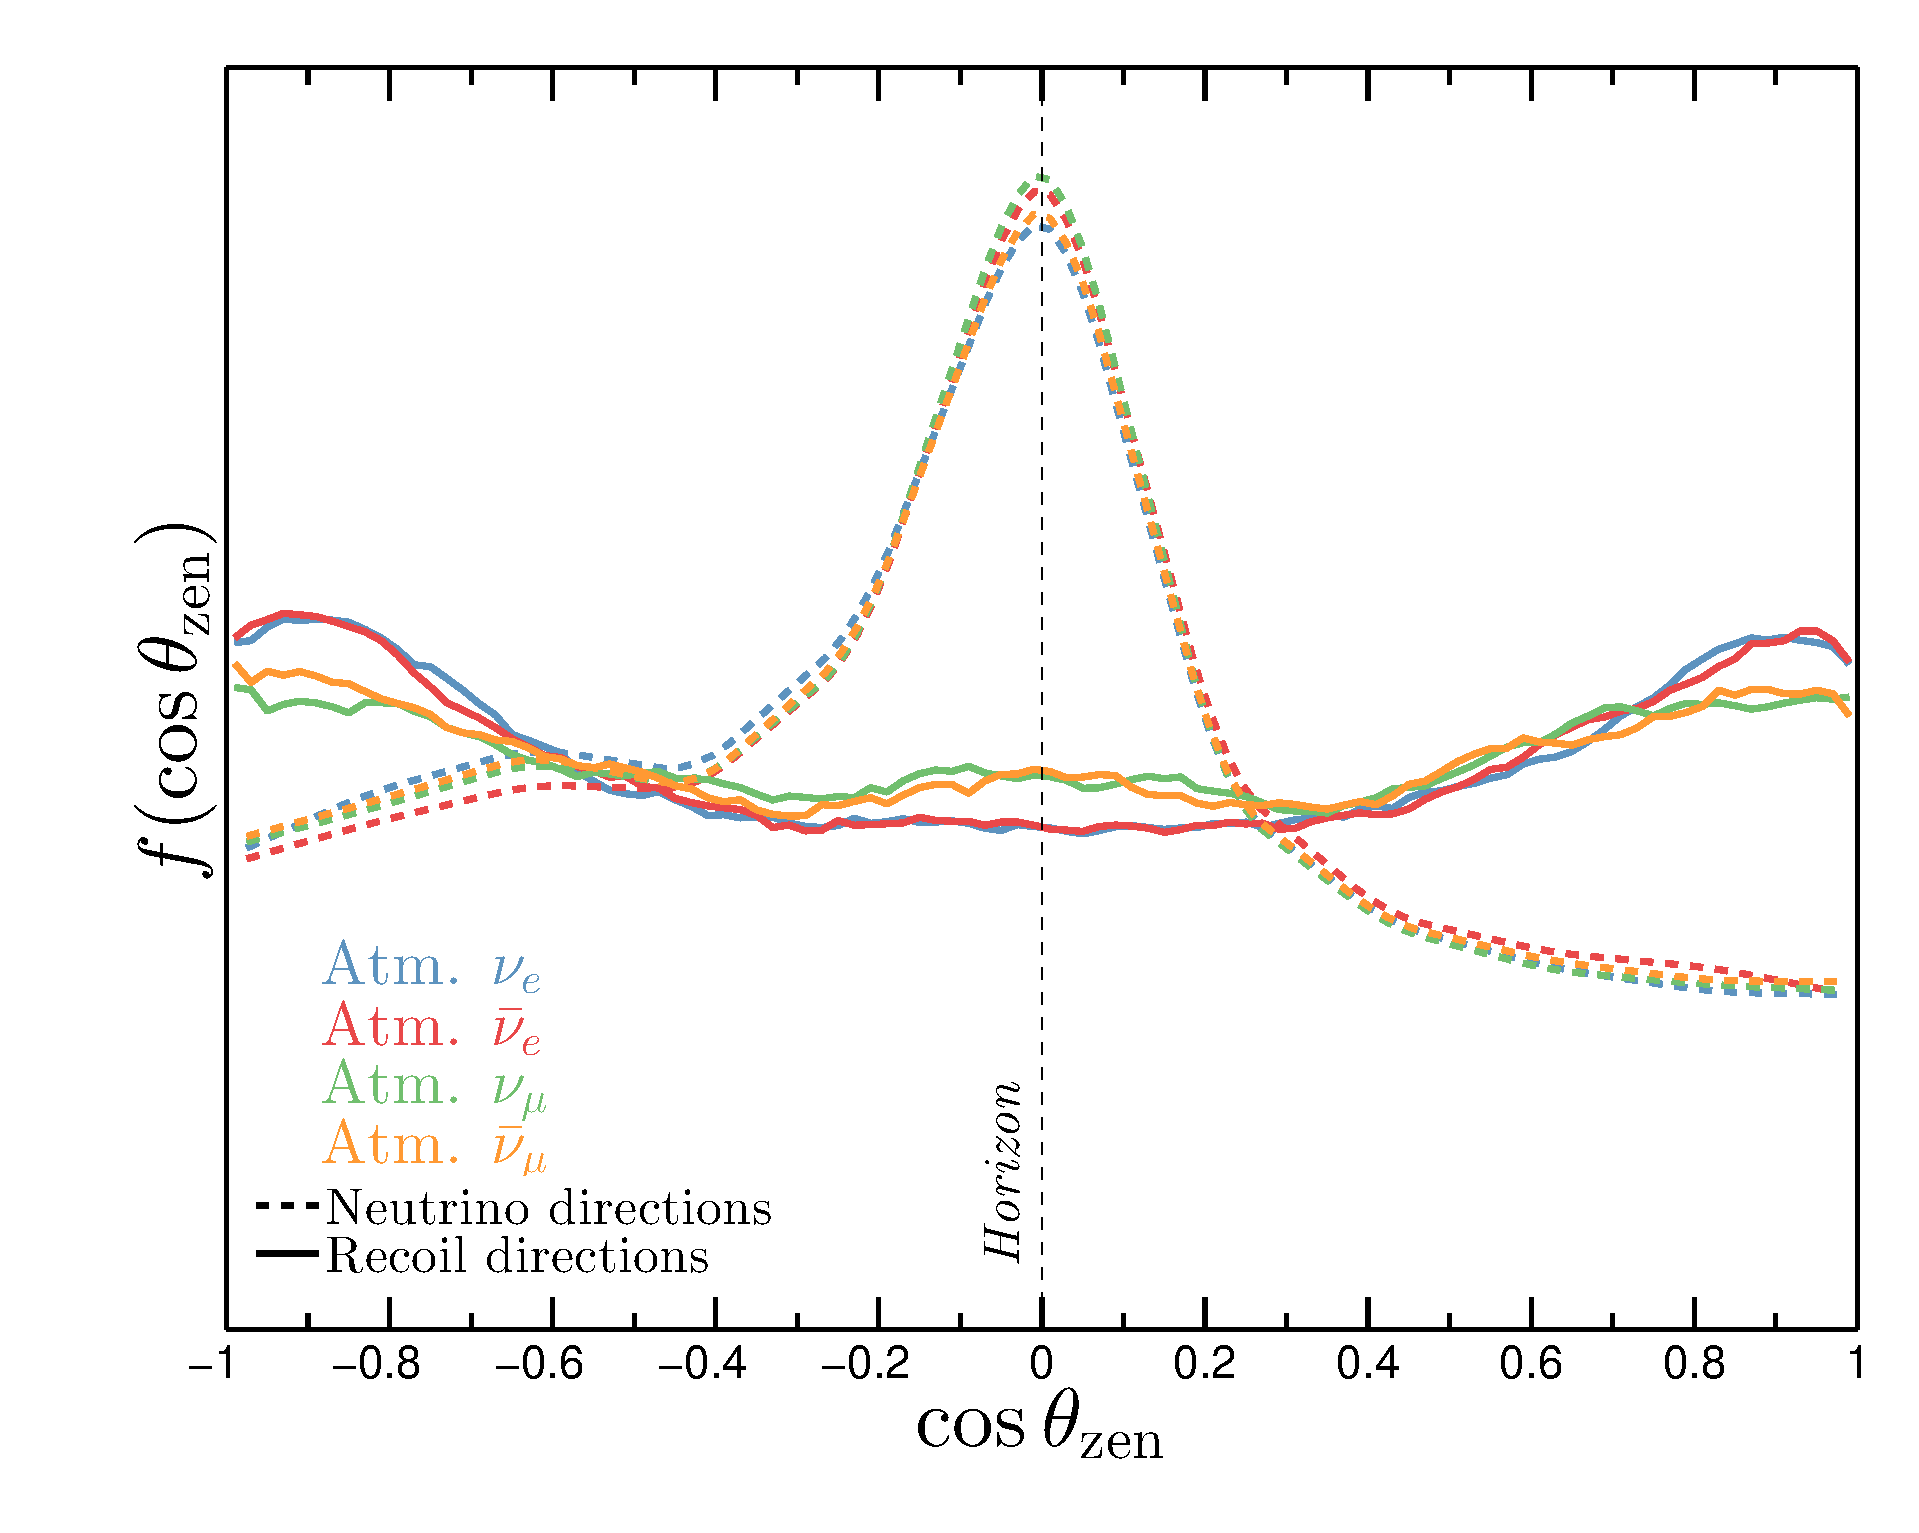
\includegraphics[trim = 0mm 0 0mm 0mm, clip, width=0.8\textwidth,angle=0]{Figures/AtmNu_zenith.eps}
\caption[Atmospheric neutrino directionality]{Angular distributions of atmospheric neutrino and their subsequent recoils. We show distributions as a function of zenith angle $\theta_{\rm zen}$ for incoming neutrinos (dashed lines) and xenon recoils above $E_{\rm th} = 5$ keV (solid lines) generated using a Monte-Carlo scattering simulation (Appendix~\ref{app:scattering}). The four lines in each case correspond to the four species of atmospheric neutrino, $\nu_e$ (blue lines), $\bar{\nu}_e$ (red lines), $\nu_\mu$ (green lines), $\bar{\nu}_\mu$ (orange lines). The incoming neutrino directions are based on the FLUKA simulations~\cite{Battistoni:2005pd}.} 
\label{fig:FLUKA}
\end{center}
\end{figure} 
Over all energies, the atmospheric neutrino flux peaks near the horizon, at zenith angle $\cos\theta_{\rm zen} \approx 0$. At high energies, the flux is very nearly symmetric about $\cos \theta_{\rm zen} \approx 0$, as at these energies the cosmic ray particles are more energetic than the rigidity cutoff. At low energies, the flux becomes asymmetric, as the flux of downward-going ($\cos \theta_{\rm zen} = 1$) neutrinos is lower than the flux of upward-going neutrinos ($\cos \theta_{\rm zen} = -1$). We consider the FLUKA results for the angular dependence of the atmospheric neutrino flux at energies relevant for direct detection experiments~\cite{Battistoni:2002ew}. In Fig.~\ref{fig:FLUKA} we show the angular spectrum of the atmospheric neutrino flux which exhibits the aforementioned dependence on zenith angle. The flux is assumed to be symmetric with azimuthal angle.

As we will discuss below we find that when the flux of atmospheric neutrinos is convolved with the coherent neutrino-nucleus scattering cross section, the angular dependence becomes washed out and the recoil spectrum depends only weakly on direction (when compared with other neutrino components and particularly WIMP recoils). Because this angular dependence is close to isotropic and will not undergo the characteristic daily transit across the sky due to the rotation of the Earth, including it will not greatly affect the discrimination between atmospheric neutrinos and WIMPs. In principle there should be a seasonal variation in the neutrino flux based on the atmospheric temperature which induces an additional time modulation, e.g. Ref.~\cite{Tilav:2010hj}. However the exact time dependence of this effect at the location of our mock experiment (Modane Underground Laboratory, France) is not known. Furthermore these variations appear to be smaller than either the WIMP or Solar neutrino modulation which are already very small effects. Hence for our analysis we model the atmospheric flux as both isotropic and constant in time,
\begin{equation}
  \frac{\textrm{d}^2 \Phi}{\textrm{d}E_\nu \textrm{d}\Omega_\nu} = \frac{1}{4\pi}\frac{\textrm{d} \Phi}{\textrm{d} E_\nu}  \,.
\label{eq:ATMDSNBflux}
\end{equation}



{\bf Diffuse supernova neutrinos}: For WIMP masses between 10 and 30 GeV, the neutrino floor is induced by the subdominant diffuse supernova neutrino background (DSNB), from all supernova explosions in the history of the Universe. The DSNB flux is the integral of the rate density for core-collapse supernova $R_{\rm SN}$ as a function of redshift $z$, with the neutrino spectrum per supernova $\Phi_{\rm SN}$~\cite{Beacom:2010kk},
\begin{equation}
 \frac{\textrm{d}\Phi}{\textrm{d}E_\nu} = \int_0^\infty \left[(1+z) \Phi_{\rm SN}(E_\nu(1+z))\right]\left[R_{\rm SN}(z)\right] \bigg|\frac{\textrm{d}t}{\textrm{d}z}\bigg| \textrm{d}z \, .
\end{equation}
where $|\textrm{d}t/\textrm{d}z|^{-1} = H_0(1+z)[\Omega_\Lambda + \Omega_m(1+z)^3]^{1/2}$ is the differential `look-back' time. The resulting spectra have a roughly Fermi-Dirac form with temperatures in the range 3~-~8~MeV. We use the following temperatures for each neutrino flavour given by Ref.~\cite{Beacom:2010kk}: $T_{\nu_e}~=~3$~MeV, $T_{\bar{\nu}_e}~=~5$~MeV and $T_{\nu_x}~=~8$~MeV, where $\nu_x$ represents the four remaining neutrino flavours. Motivated by theoretical estimates we take a systematic uncertainty on the DSNB flux of 50\%. The DSNB is believed to be isotropic and constant over time, therefore its angular dependence can be expressed, as with the atmospheric neutrinos, using Eq.~(\ref{eq:ATMDSNBflux}).  


{\bf Other neutrinos}: We have summarised the three sources of neutrino that are most important for the discovery limits of dark matter experiments, although there are a few sources we do not consider. Most notably neutrinos from individual Milky Way supernovae would also certainly show up in direct detection experiments if the explosion were close enough to Earth. In fact existing and future ton-scale detectors are in a position to perform novel supernova physics in the event of a Galactic supernova~\cite{Lang:2016zhv}. We do not consider distinct supernovae neutrinos as a background here as the events would probably be coincident with a large nearby explosion.

We do not need to consider cosmological relic neutrinos as their energies are well below the thresholds of all current and near future experiments, however we note that the motion of the Milky Way with respect to the rest frame of the CMB would give rise to a signature direction dependence as with the primary CMB dipole~\cite{Safdi:2014rza,Domcke:2017aqj}.
We also neglect reactor neutrinos as it is unlikely that a direct detection experiment would be situated close enough to a nuclear reactor for them to be a significant background. We also ignore sources of geoneutrinos from radioactive decays which produce a subdominant flux from the ground with energies below 4.5 MeV~\cite{Monroe:2007xp}. Finally, fluxes of much higher energy extragalactic neutrinos from, for example, active galactic nuclei or gamma-ray bursts, have fluxes well below the sensitivity of a dark matter experiment~\cite{Gaisser:1994yf,Halzen:2002pg,Aartsen:2014gkd}.



\subsection{Coherent neutrino-nucleus elastic scattering}
We only consider the neutrino background from coherent neutrino-nucleus elastic scattering (CNS) as it produces nuclear recoils in the keV energy scale which cannot be distinguished from a WIMP interaction\footnote{We neglect neutrino-electron elastic scattering, mostly induced by $pp$ neutrinos, as it has been shown to only marginally affect the discovery potential of experiments with limited nuclear/electronic recoil discrimination for WIMP masses above 100 GeV~\cite{Billard:2013qya}.}. CNS proceeds via a neutral current, and as shown by Freedman~\cite{Freedman:1973yd} and subsequently Drukier \& Stodolsky~\cite{Drukier:1983gj} has a coherence effect at low momentum transfer that approximately scales with the number of neutrons squared. At higher recoil energies, generally above a few tens of keV, the loss of coherence is described by the nuclear form factor $F(E_r)$, for which we again use the standard Helm ansatz~\cite{Lewin:1995rx} which is an excellent approximation at these low energies~\cite{Vietze:2014vsa}. The differential cross section as a function of the nuclear recoil energy ($E_r$) and neutrino energy ($E_\nu$) is given by 
\be
  \frac{\textrm{d} \sigma}{\textrm{d}E_r}(E_r,E_\nu) = \frac{G_F^2}{4 \pi} Q^2_W m_N \left(1-\frac{m_N E_r}{2 E_\nu^2} \right) F^2(E_r) \,,
\ee
where $Q_W = A-Z - (1-4\sin^2\theta_W) Z$ is the weak nuclear hypercharge of the nucleus, $G_F$ is the Fermi coupling constant, $\theta_W$ is the weak mixing angle and $m_N$ is the target nucleus mass. We assume CNS to be a pure standard model interaction and do not consider any exotic mediators as in, for example, Refs.~\cite{Cerdeno:2016sfi,Bertuzzo:2017tuf}.

The directional cross section can be written by noting that the scattering has azimuthal symmetry about the incoming neutrino direction so $\rm{d}\Omega_\nu = 2\pi \,\rm{d}\cos\beta$ and imposing the kinematical expression for the scattering angle, $\beta$, between the neutrino direction, $\hat{{\bf q}}_\nu$, and the recoil direction, $\hat{{\bf q}}_r$,
\be
 \cos\beta = \hat{{\bf q}}_r \cdot \hat{{\bf q}}_\nu = \frac{E_\nu + m_N}{E_\nu}\sqrt{\frac{E_r}{2 m_N}} \,,
\label{eq:kinematics}
\ee 
with $\beta$ in the range $(0,\pi/2)$, using a delta function,
\be
  \frac{\textrm{d}^2 \sigma}{\textrm{d}E_r \textrm{d}\Omega_r} = \frac{\textrm{d} \sigma}{\textrm{d}E_r} \, \frac{1}{2 \pi}\, \delta\left(\cos\beta - \frac{E_\nu + m_N}{E_\nu} \sqrt{\frac{E_r}{2 m_N}}\right) \,.
\label{eq:doublecrosssection}
\ee
The maximum recoil energy, $E_r^{\rm max}$, can be obtained by setting $\beta = 0$ in Eq.~(\ref{eq:kinematics}),
\be
E_r^{\rm max} = \frac{2 m_N E_\nu^2}{(E_\nu + m_N)^2} \approx \frac{2E_\nu^2}{m_N + 2E_\nu} \,.
\ee
The maximum recoil energies produced by the different types of neutrino for a xenon target are shown in Table~\ref{tab:neutrino}.

\par The CNS event rate per unit detector mass, as a function of the recoil energy, direction and time, is given by the convolution of the double differential CNS cross section and the directional neutrino flux,
\be\label{eq:nu_directionalrate}
  \frac{\textrm{d}^2 R(t)}{\textrm{d}E_r \textrm{d}\Omega_r} =  \frac{1}{m_N} \int_{E_\nu^{\rm min}} \frac{\textrm{d}^2 \sigma}{\textrm{d}E_r \textrm{d}\Omega_r}\times\frac{\textrm{d}^2 \Phi(t)}{\textrm{d}E_\nu \textrm{d}\Omega_\nu} \textrm{d}E_\nu \textrm{d}\Omega_\nu \,,
\ee
where $E_\nu^{\rm min} = \sqrt{m_NE_r/2}$ is the minimum neutrino energy required to generate a nuclear recoil with energy $E_r$.

The directional event rate for Solar neutrinos is found by substituting Eqs.~(\ref{eq:solarneutrinoflux_directional}), (\ref{eq:kinematics}) and (\ref{eq:doublecrosssection}) into Eq.~(\ref{eq:nu_directionalrate}) and integrating over the neutrino direction $\Omega_\nu$,
\begin{align}
  \frac{\textrm{d}^2 R(t)}{\textrm{d}E_r \textrm{d}\Omega_r} &= \frac{1}{2\pi m_N}\left[ 1 + 2\epsilon\cos\left(\frac{2\pi(t- t_\nu)}{T_\nu}\right) \right]  \nonumber \\
&\times \int \frac{\textrm{d} \sigma}{\textrm{d}E_r}  \frac{\textrm{d} \Phi}{\textrm{d} E_\nu} \delta\left(\hat{{\bf q}}_r \cdot \hat{{\bf q}}_\odot(t) - \frac{E_\nu + m_N}{E_\nu} \sqrt{\frac{E_r}{2 m_N}}\right) \textrm{d}E_\nu \,.
\label{eq:intermediate}
\end{align}
The delta function can then be rewritten as
\be
  \delta\left(\hat{{\bf q}}_r \cdot \hat{{\bf q}}_\odot(t) - \frac{E_\nu + m_N}{E_\nu} \sqrt{\frac{E_r}{2 m_N}}\right) =  \frac{1}{E_\nu^\textrm{min}} \, \,\delta \left(x + \frac{1}{\mathcal{E}(t)}\right) \, ,
\label{eq:delta}
\ee
where we have defined $x = -1/E_\nu$ and,
\be
  \frac{1}{\mathcal{E}(t)} = \frac{\hat{{\bf q}}_r \cdot \hat{{\bf q}}_\odot(t)}{E_\nu^\textrm{min}} - \frac{1}{m_N} \,.
\ee

Finally, by substituting Eq.~(\ref{eq:delta}) into Eq.~(\ref{eq:intermediate}), integrating over $x$ and converting back to $E_\nu$, we obtain an analytic expression for the directional event rate from Solar neutrinos,
\begin{equation}
  \frac{\textrm{d}^2 R(t)}{\textrm{d}E_r \textrm{d}\Omega_r} =  \frac{1}{2\pi m_N}\left[ 1 + 2\epsilon\cos\left(\frac{2\pi(t- t_\nu)}{T_\nu}\right) \right]  \frac{\mathcal{E}(t)^2}{ E_\nu^\textrm{min}} \left(\frac{\textrm{d} \sigma}{\textrm{d}E_r}\frac{\textrm{d} \Phi}{\textrm{d} E_\nu}\right)\bigg|_{E_\nu = \mathcal{E}(t)} \,,
\label{eq:solarnu}
\end{equation}
for $\cos^{-1}(\hat{{\bf q}}_r \cdot \hat{{\bf q}}_\odot(t)) < \pi/2$ and 0 otherwise.

In the case of the atmospheric and diffuse supernova neutrinos, as we have assumed their fluxes to be isotropic and constant over time, the directional event rate is simply given by substituting Eqs.~(\ref{eq:ATMDSNBflux}) and (\ref{eq:doublecrosssection}) into Eq.~(\ref{eq:nu_directionalrate}) and integrating over the neutrino direction $\Omega_\nu$ leading to
\be
\frac{\textrm{d}^2 R}{\textrm{d}E_r \textrm{d}\Omega_r} = \frac{1}{4\pi m_N} \int_{E_{\nu}^\textrm{min}} \frac{\textrm{d} \sigma}{\textrm{d}E_r} \frac{\textrm{d} \Phi}{\textrm{d}E_\nu } \textrm{d}E_\nu \,. 
\label{eq:isonu}
\ee


\subsection{Resulting signals}
\label{sec:nufloor_signals}
 \begin{figure}
\begin{center}
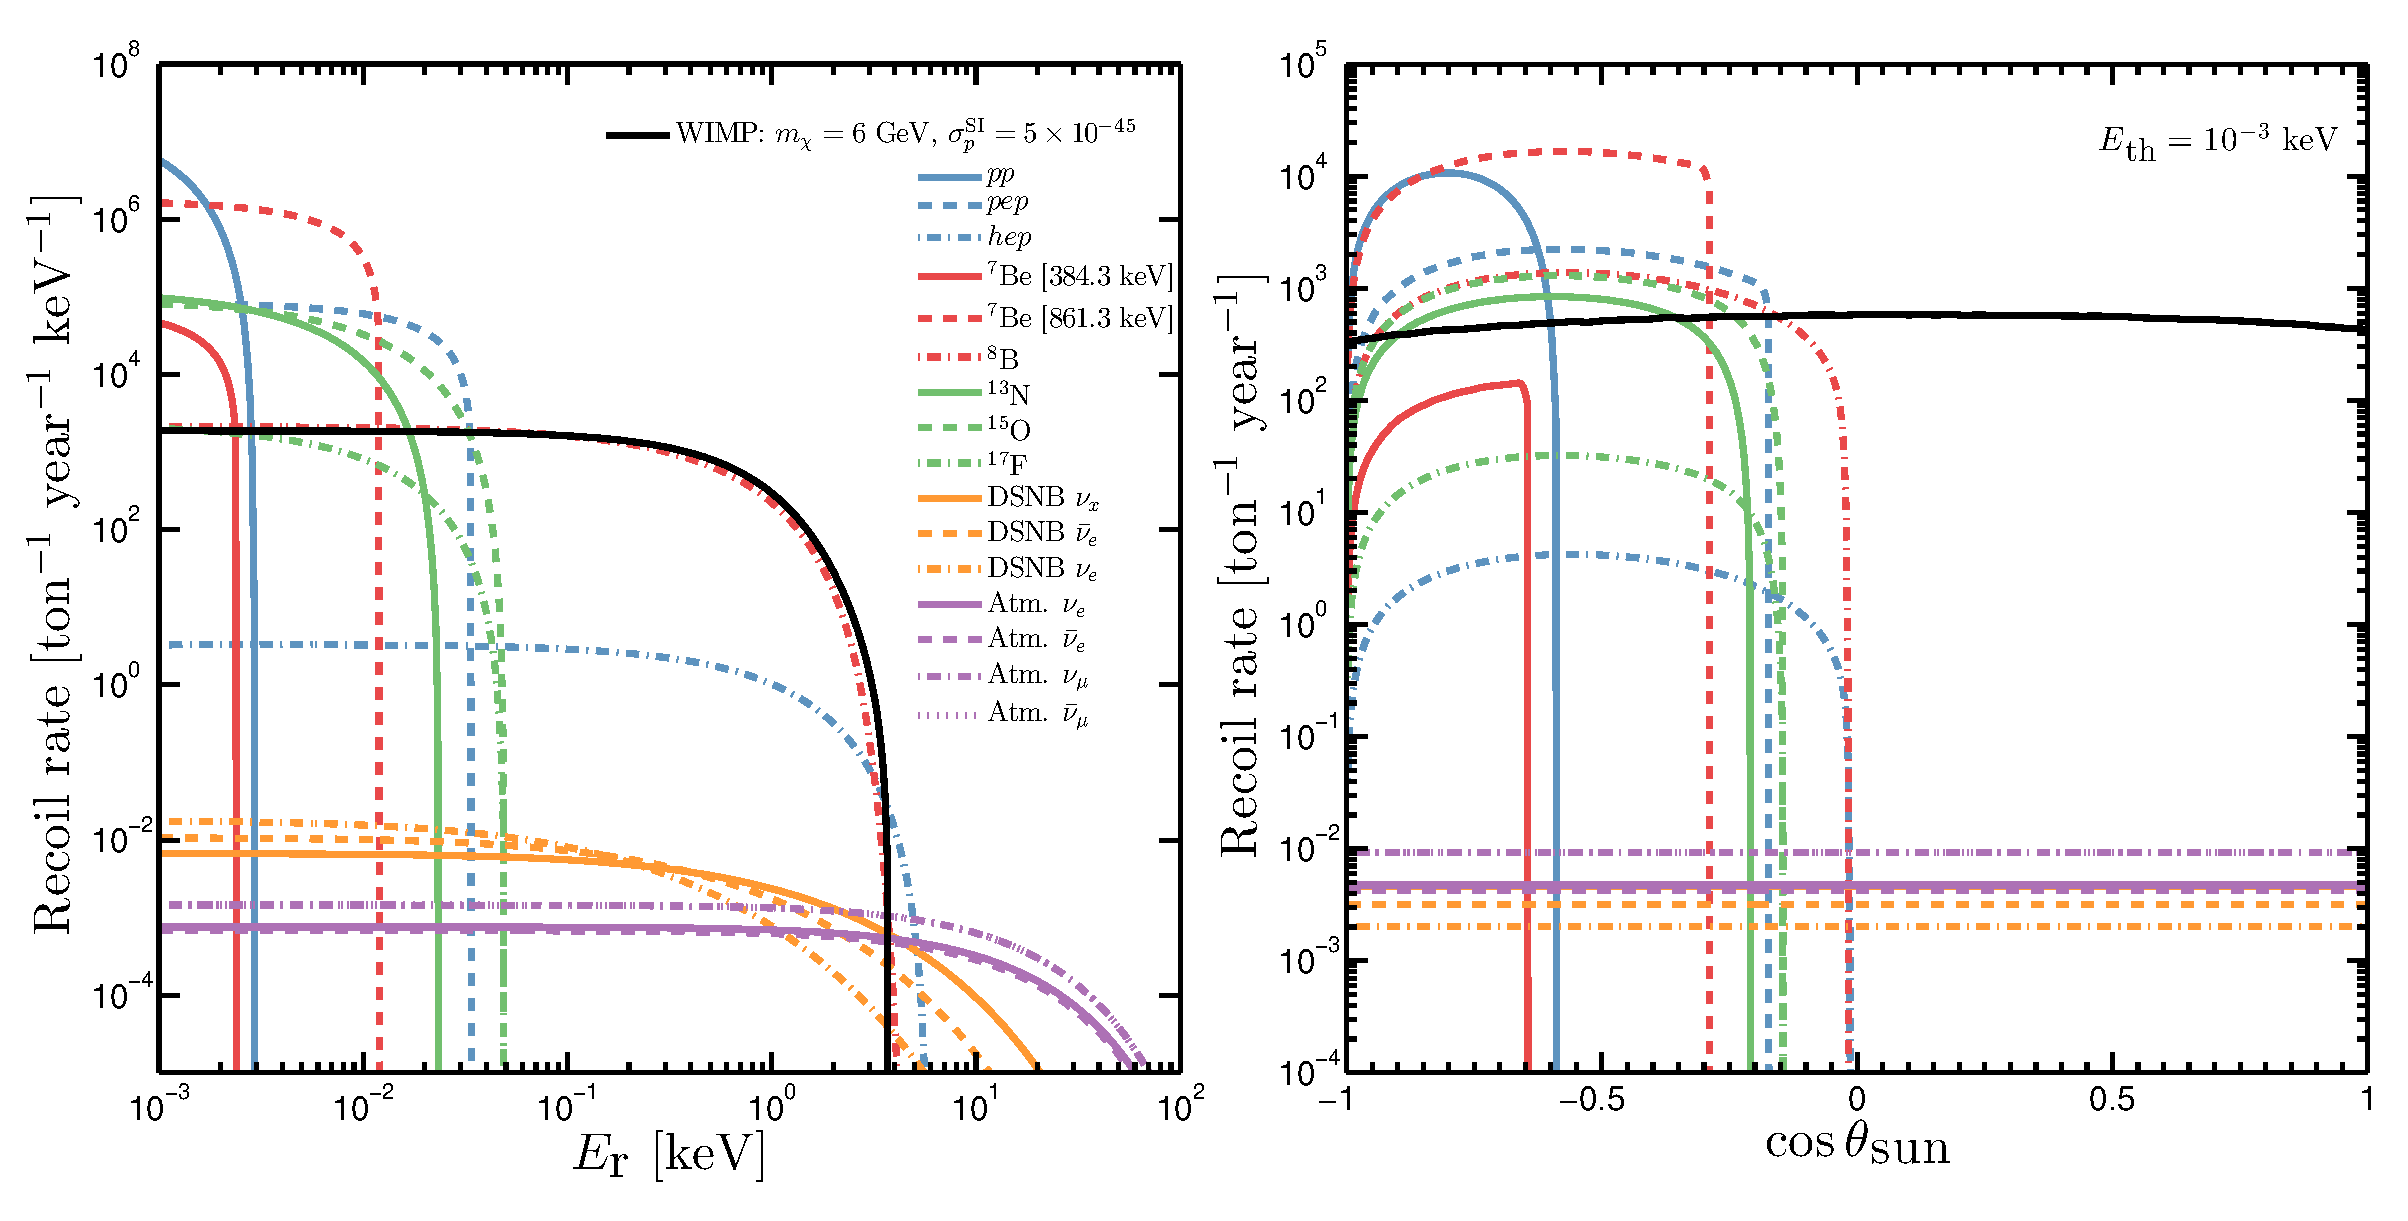
\includegraphics[trim = 0mm 0 0mm 0mm, clip, width=0.98\textwidth,angle=0]{Figures/NeutrinoAll_1D_recoilrates.eps}
\caption[Neutrino and $m_{\chi} = 6 \, {\rm GeV}$ WIMP nuclear recoil rates]{Neutrino and $m_{\chi} = 6 \, {\rm GeV}$ WIMP nuclear recoil rates for a xenon target as a function of recoil energy, $E_r$, (left) and cosine of the angle between the Solar vector and recoil vector, $\cos \theta_\textrm{sun}$, (right)  obtained by integrating the differential recoil spectrum over angle and energy respectively. The atmospheric and DSNB neutrino fluxes are taken to be isotropic. In order to show all types of neutrino we integrate above $E_r = 1$~eV.} 
\label{fig:neutrinorates}
\end{center}
\end{figure} 
The neutrino event rates as a function of energy and angle between Solar and recoil directions, $\cos{\theta_\textrm{sun}} = -\hat{\bf{q}}_r\cdot\hat{\bf{q}}_\odot$, obtained by integrating Eqs.~(\ref{eq:solarnu}) and ~(\ref{eq:isonu}) over direction and energy respectively are shown in Fig.~\ref{fig:neutrinorates}. Also shown is the recoil rate for a 6 GeV WIMP, showing the similarity between this spectrum and the spectrum of $^8$B neutrino recoils. The isotropic DSNB and atmospheric recoil rates are flat whereas the event rates of Solar neutrinos are highly anisotropic. The curves corresponding to the monoenergetic neutrinos ($^7$Be and $pep$) have a sharp cutoff in their directionality due to the finite energy threshold. From Fig.~\ref{fig:neutrinorates} one can already anticipate that the degeneracy between Solar neutrino and WIMP events from an energy-only analysis will be almost completely removed with the addition of directional information.


 \begin{figure}
\begin{center}
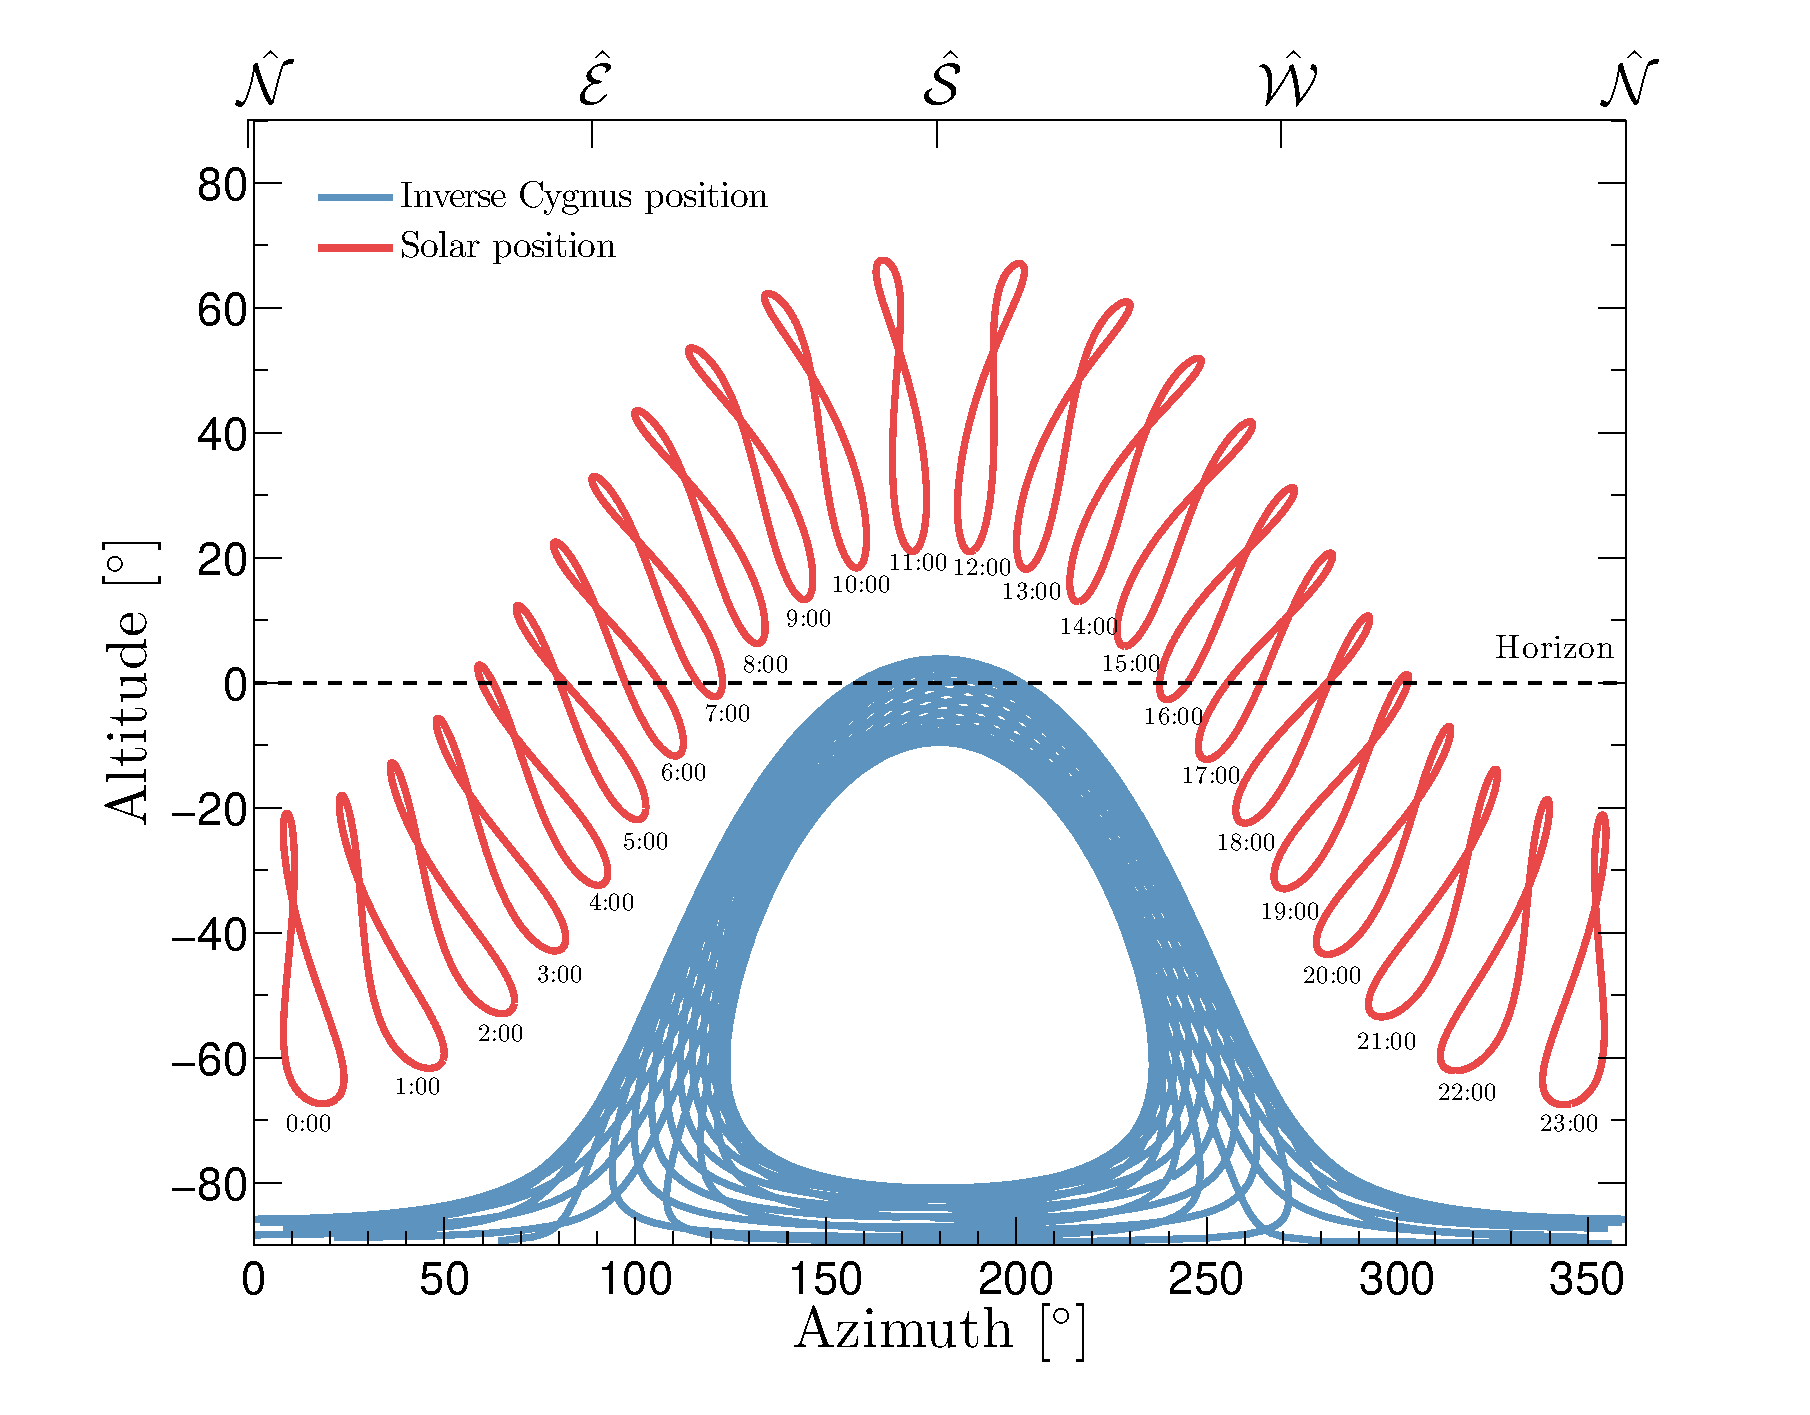
\includegraphics[trim = 15mm 5mm 18mm 5mm, clip, width=0.8\textwidth,angle=0]{Figures/SolarCygnusDirections.eps}
\caption[The evolution of the position of the Sun and Cygnus in the sky]{The position in the sky, in terms of Altitude and Azimuth, of the Sun (red) and the inverse of the position of the constellation Cygnus (corresponding to the direction -$\bf{v}_\textrm{lab}$) (blue) as observed from the Modane underground laboratory (latitude $45.2^{\circ}$). The points show the position at measurements made every hour from the 1st January 2015 0:00 until 31st December 2015 23:00. The Solar position traces out 24 analemmas for observations made at each hour of the day over the course of a year. The dashed horizontal line is the horizon. As demonstrated here, the Sun's position does not coincide with that of Cygnus at any time.} 
\label{fig:solarcygnus}
\end{center}
\end{figure} 
Figure~\ref{fig:solarcygnus} shows the position in the sky of the Sun and the inverse of the position of Cygnus (i.e. $-\bf{v}_\textrm{lab}$), as observed from the Modane underground laboratory (latitude $45.2^{\circ}$). The points show the position at observations made every hour from the 1st January 2015 0:00 until 31st December 2015 23:00. The Solar position traces out 24 `analemmas' which are lines connecting observations of the Sun's position at the same hour each day over a full year. As we see here, the Sun's position does not coincide with that of Cygnus at any time suggesting that a directional experiment should in principle be able to disentangle the WIMP from the Solar neutrino contributions in the observed data. In fact the angular separation between the peak WIMP direction and the peak neutrino direction undergoes a sinusoidal modulation over the course of the year that varies from $60^{\circ}$ in February to $120^{\circ}$ in September.

\begin{figure}
\begin{center}
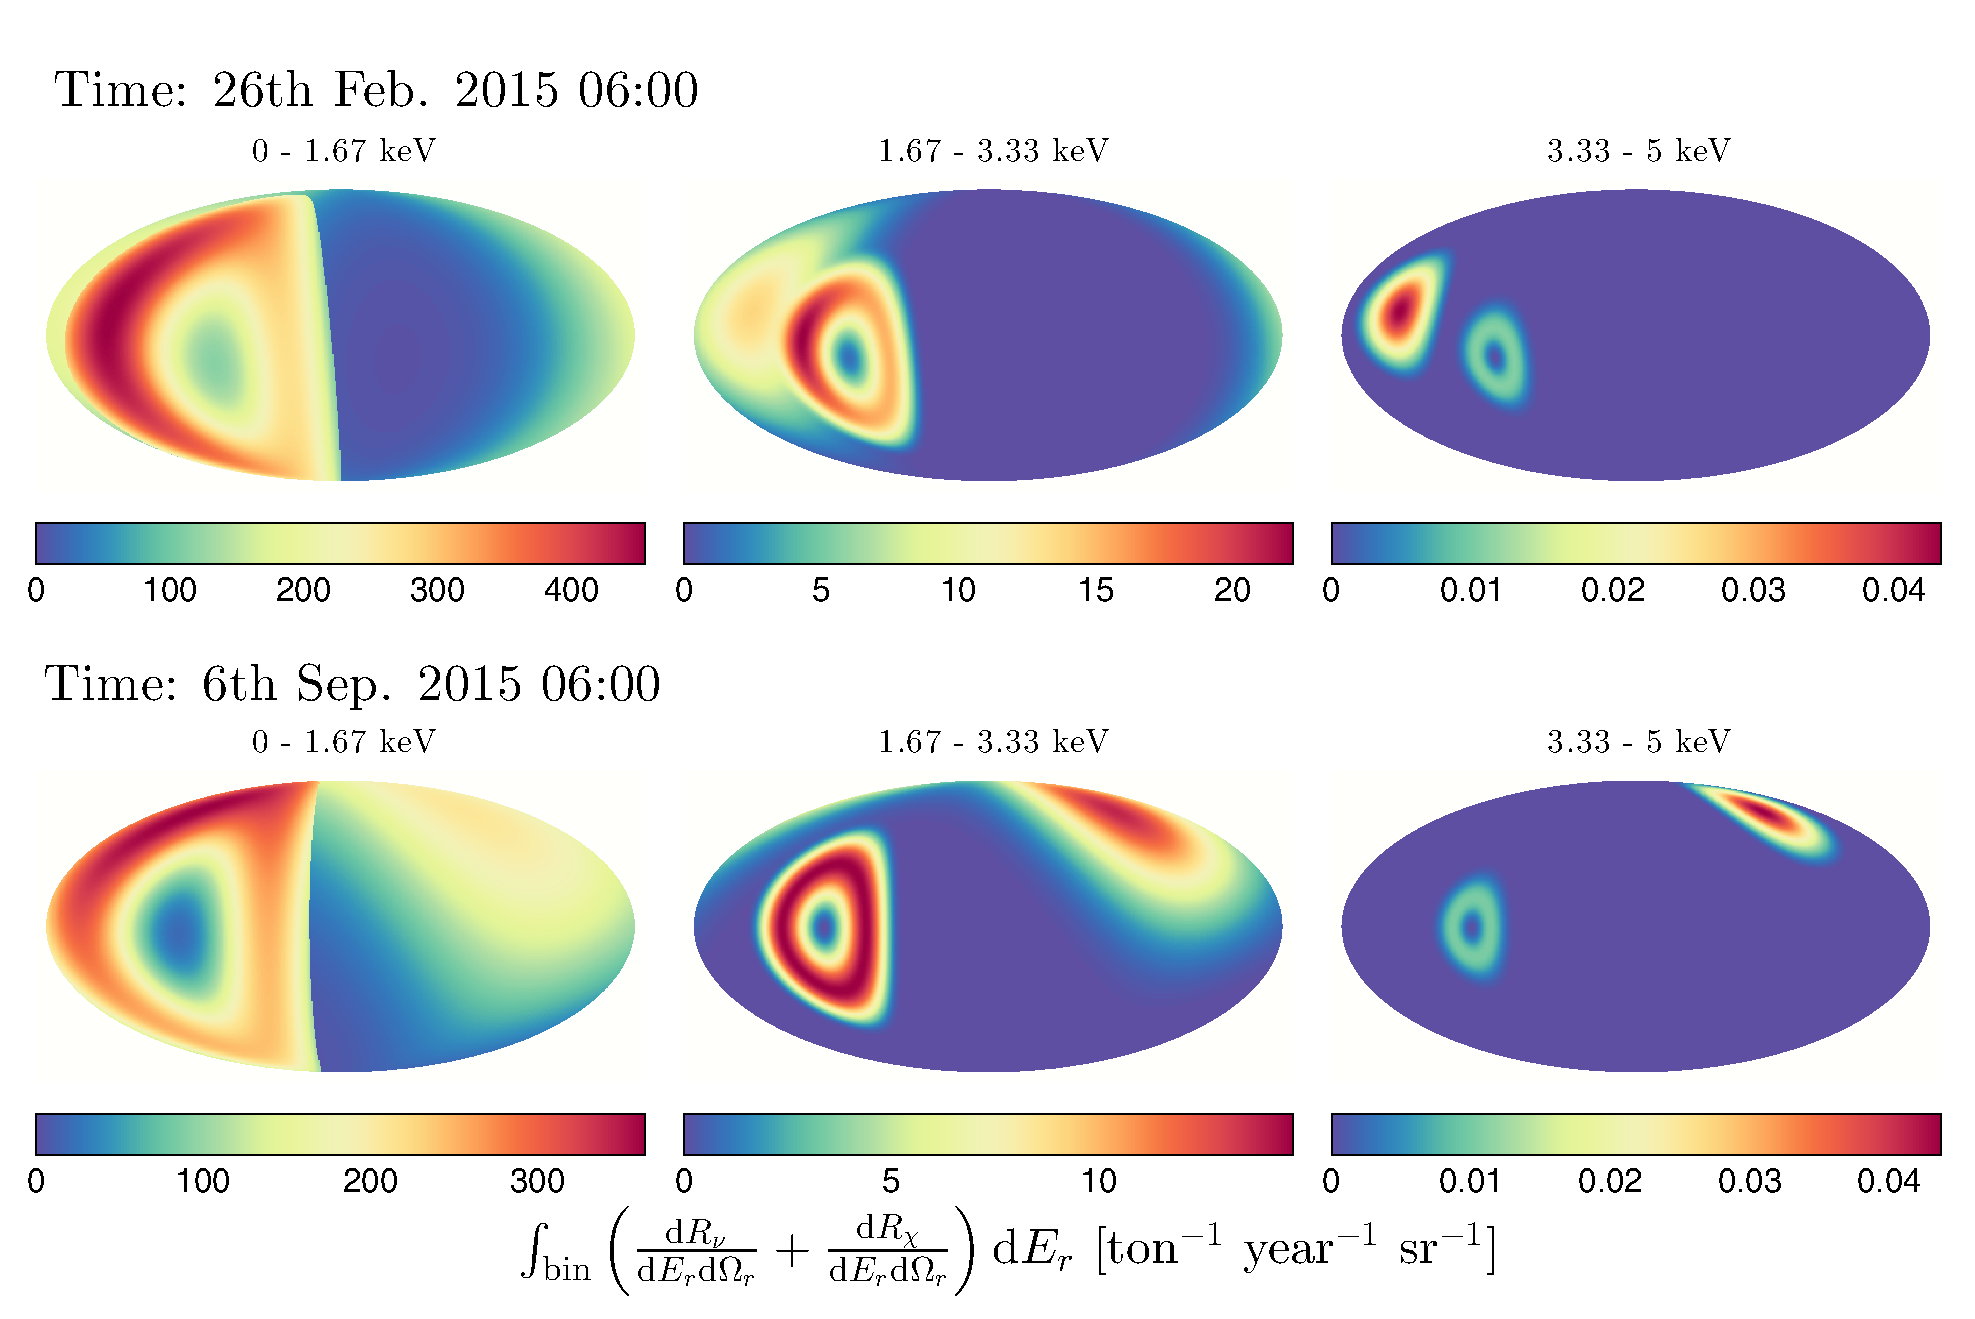
\includegraphics[trim = 0mm 0mm 0mm 0mm, clip, width=\textwidth,angle=0]{Figures/mollweide_minmax_times.eps}
\caption[Mollweide projections of the WIMP and $^8$B neutrino event rates]{Mollweide projections of the WIMP and $^8$B neutrino angular differential event rate ($R_\chi$ and $R_\nu$ respectively) integrated within (from left to right) three equally sized energy bins spanning the range $E_{r} = 0 \,$ to $5 \, {\rm keV}$, for a WIMP with mass $m_{\chi} = 6 \, {\rm GeV}$ and $\sigma^{\rm SI}_p = 5 \times 10^{-45} \, {\rm cm}^2$ and a ${\rm Xe}$ target.
The top row shows the signal on February 26th, when the separation between the directions of the Sun and Cygnus is smallest ($\sim 60^{\circ}$), and the bottom row on September 6th, when the separation is largest ($\sim 120^{\circ}$). The WIMP contribution is to the left of the neutrino contribution on the top row and to the right on the bottom row. The Mollweide projections are of the event rate in the laboratory coordinate system with the horizon aligned horizontally and the zenith and nadir at the top and bottom of the projection respectively.} 
\label{fig:Moll}
\end{center}
\end{figure}
Figure~\ref{fig:Moll} shows Mollweide projections of the laboratory frame angular differential event rate from a 6 GeV WIMP plus $^8$B Solar neutrinos,  at the times when the separation between the directions of the Sun and Cygnus are smallest and largest. Even at the time of smallest separation, the WIMP and neutrino recoil distributions can be easily distinguished as long as the angular resolution is better than a few tens of degrees. Although we only show the rates for $^8$B neutrino induced recoils, the angular distributions for other Solar neutrinos are very similar as neutrinos can only induce a recoil with an angle in the range $(0,\pi/2)$ from their incident direction. Additionally, the angular dependence of the recoil spectra is correlated with energy as can be seen going from the left to the right hand panels. For both the WIMP and neutrino recoils the angular spread decreases with increasing energy i.e. the highest energy recoils have the smallest angle between the incoming particle direction and the recoil direction.





\section{The neutrino floor}\label{sec:nufloor_nufloor}
\subsection{Discovery limits}
We now introduce the analysis methodology and the calculation of the neutrino floor as a discovery limit to {\it non}-directional detection experiments. Discovery limits were first introduced in Ref.~\cite{Billard:2011zj} and are defined such that if the true WIMP model lies above the limit then a given experiment has a 90\% probability to achieve at least a 3$\sigma$ WIMP detection. As such they are analogous to exclusion limits made by a particular experiment in practice however they relate to predictions for the range of WIMP cross sections to which a hypothetical experiment will be sensitive. The neutrino floor is a theoretical limit which is found by computing a discovery limit for an experiment that has a neutrino background. We describe this procedure in full in Appendix~\ref{app:likelihood}.

To calculate the neutrino floor we adopt a binned likelihood with $N_\textrm{bins}=100$ to allow us to efficiently perform our analysis with large numbers of neutrino events. The likelihood is written as the product of the Poisson probability distribution function ($\mathscr{P}$) for each bin, multiplied by individual likelihood functions parameterising the uncertainties on each neutrino flux normalisation and each astrophysical parameter,
\begin{align}\label{eq:likelihood}
 \mathscr{L}(m_\chi,\sigma^{\rm SI}_p,\boldsymbol{\Phi},\boldsymbol{\Theta}) = \prod_{i=1}^{N_\textrm{bins}} \mathscr{P} \left(N_\textrm{obs}^i \bigg| N^i_\chi + \sum_{j=1}^{n_\nu} N^{i}_\nu(\phi^j)\right) 
\prod_{j=1}^{n_\nu} \mathcal{L}(\Phi^j)
\prod_{k=1}^{n_\theta} \mathcal{L}(\theta^k) \, .
\end{align}
Where $\boldsymbol{\Phi} = \{ \Phi^1, ..., \Phi^{n_\nu} \}$ are the neutrino fluxes for each of the $n_\nu$ neutrino types and $\boldsymbol{\Theta} = \{\theta^1, ..., \theta^{n_\theta} \}$ contains the $n_\theta$ astrophysical uncertainties under consideration which will vary depending on the choice of velocity distribution e.g. the standard halo model: $\boldsymbol{\Theta}_\textrm{SHM} = \{ v_0,\vesc,\rho_0 \}$. The functions $\mathcal{L}(\phi^j)$ are the Gaussian parameterisations for each neutrino flux (see Table~\ref{tab:neutrino}) and similarly the likelihood functions $\mathcal{L}(\theta^k)$ parametrise the systematic uncertainty on each astrophysical parameter. Inside the Poisson function we have for each bin $i$, the observed number of events $N_\textrm{obs}^i$, the expected number of WIMP events $N_\chi^i$ given by,
\begin{equation}\label{eq:nchi}
N_\chi^i(m_\chi,\sigma^{\rm SI}_p,\boldsymbol{\Theta}) =\mathcal{E}\int_{E_{i}}^{E_{i+1}} \frac{\textrm{d} R_\chi}{\textrm{d}E_r} \textrm{d}E_r \, ,
\end{equation}
and $N_\nu^i(\phi^j)$ which is the expected number of neutrino events from the $j$th neutrino species,
\begin{equation}
N^{i}_\nu (\phi^j) = \mathcal{E}\int_{E_{i}}^{E_{i+1}} \frac{\textrm{d} R_\nu}{\textrm{d}E_r}(\phi^j) \textrm{d}E_r \, ,
\end{equation}
where $\mathcal{E}$ is the exposure of the experiment which we will quote in units of ton-year. We clarify here that the neutrino floor is not usually defined with the inclusion of any extra discrimination with timing information hence the likelihood is calculated assuming rates for WIMP and neutrinos that are constant in time. We adopt this convention to allow our neutrino floor limits to be compared with the literature. We show explicitly the added discrimination power brought by timing information in Sec.~\ref{sec:nufloor_time}.

\begin{figure}
\begin{center}
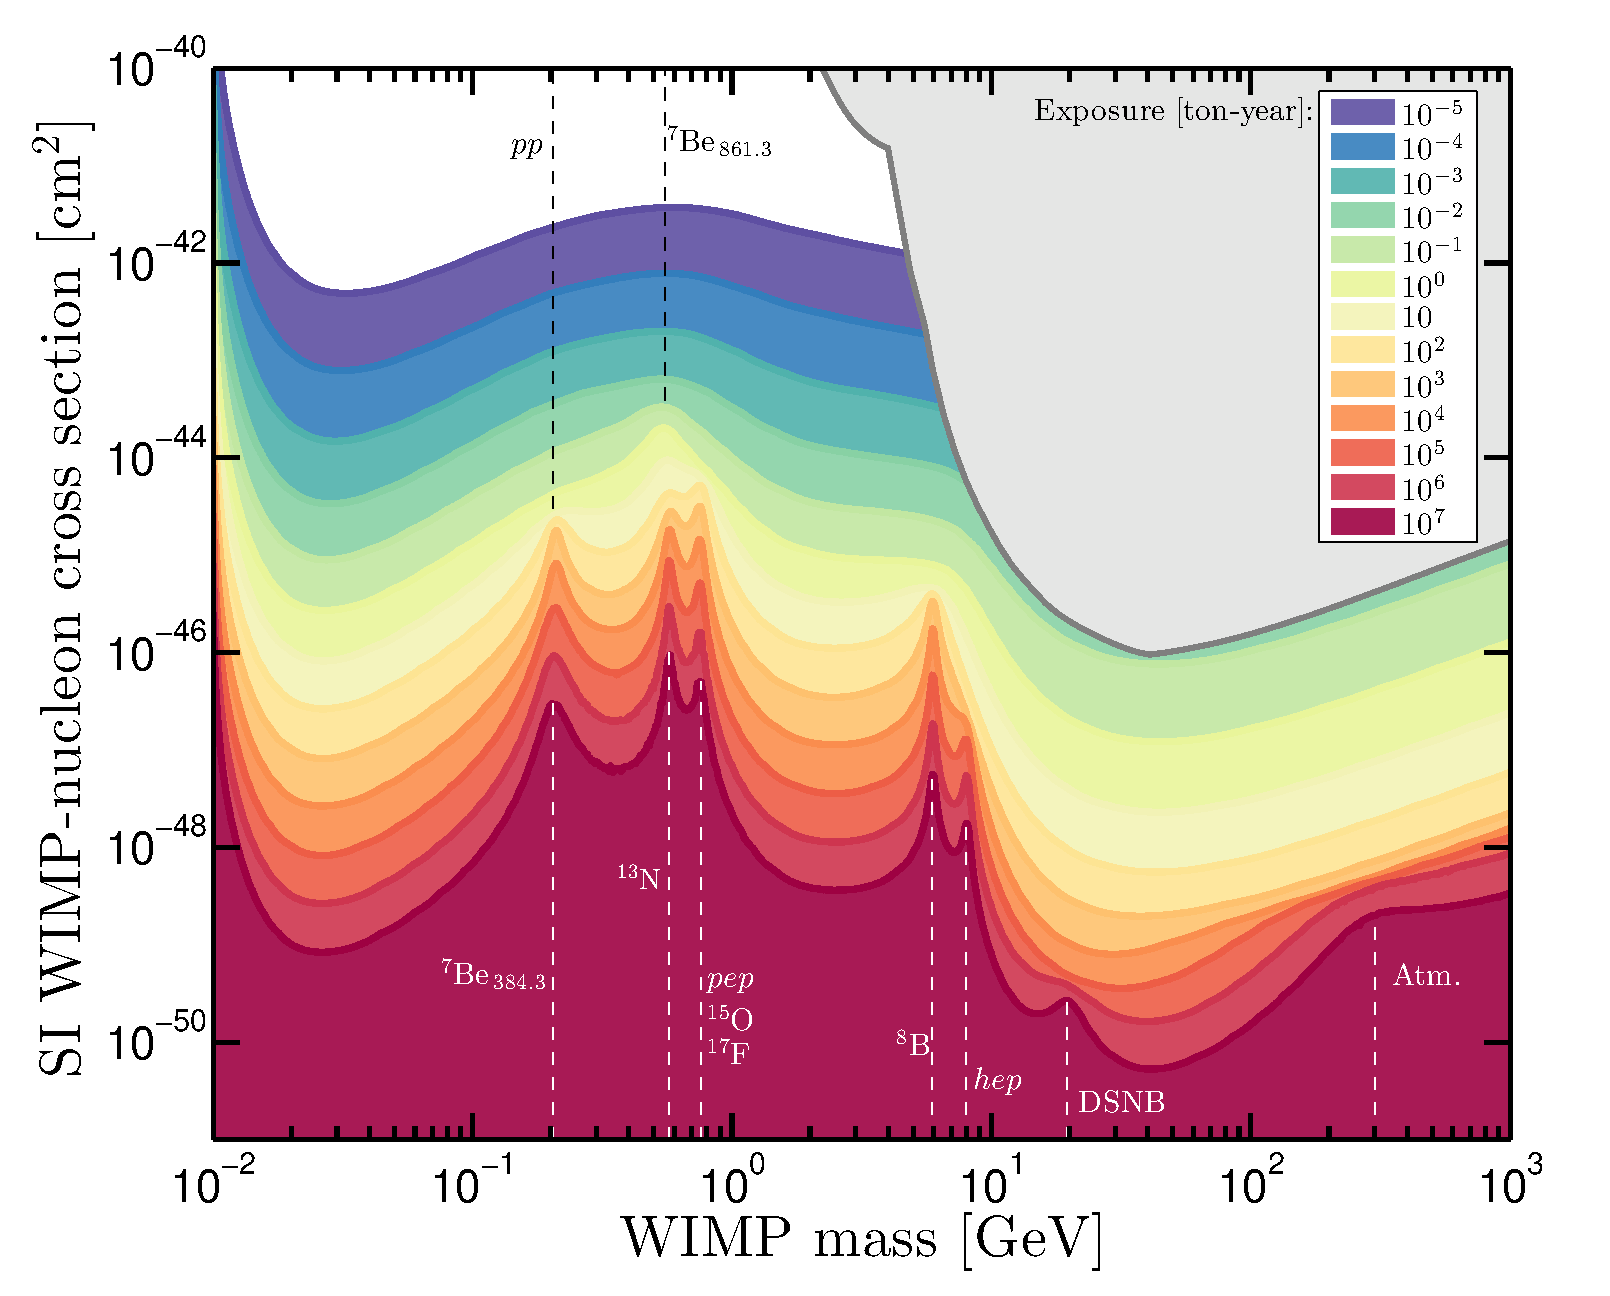
\includegraphics[trim = 0mm 0 0mm 0mm, clip, width=0.9\textwidth,angle=0]{Figures/EL_vs_mass_allNeutrinos.eps}
\caption[The complete SI xenon neutrino floor]{Illustration of the full dependence of the SI neutrino floor for a xenon target as a function of WIMP mass and detector exposure, showing the contribution from all sources of neutrino. The neutrino floor has peaks at WIMP masses where the xenon scattering rate for WIMPs and a certain neutrino source overlap. We indicate the region of this parameter space already excluded by experiments in grey.}
\label{fig:EL_vs_mass_allNeutrinos}
\end{center}
\end{figure} 
Figure~\ref{fig:EL_vs_mass_allNeutrinos} shows the full evolution of the discovery limit for a xenon experiment with an extremely low threshold (0.01 eV) to capture the neutrino floor down to $pp$ neutrino energies for completeness. It is important to note however that this Figure is merely an illustrative demonstration of each neutrino contribution as exposures of up to $10^7$ ton-years are clearly unfeasible. In Fig.~\ref{fig:EL_vs_mass_allNeutrinos} we see that the floor moves to lower cross sections as the exposure is increased as one would expect, however it acquires peaks where the WIMP recoil spectrum is mimicked by a given neutrino component. The mass at which a peak appears is dependent on the recoil energy range of the neutrino type. The cross section of the peak and how long the peak remains as exposure is increased depends on the uncertainty on the neutrino flux as well as how well the WIMP recoil event rate is mimicked by the neutrino type~\cite{Ruppin:2014bra}. With a smaller uncertainty it takes fewer WIMP events to distinguish them from neutrinos. The most important contribution to the neutrino floor is due to $^8$B neutrinos which cause a peak to appear at 6 GeV and are within the scope of upcoming direct detection experiments. There are also contributions from $hep$, atmospheric and DSNB neutrinos at higher WIMP masses which may be accessible in very large ($>100$ ton-year) experiments such as DARWIN~\cite{Aalbers:2016jon}. Finally, for low WIMP mass searches (below 1 GeV) there is a cluster of peaks due to the lower energy Solar neutrinos: $pp$, $pep$, $^7$Be, $^{15}$O, $^{13}$N and $^{14}$F.

As we displayed with Fig.~\ref{fig:WIMPlimits_SI} in Chapter~\ref{chapter:direct}, the neutrino floor also depends upon the target nucleus and whether one considers SI or SD interactions. For clarity in describing the phenomenology of the neutrino floor we show just limits for a xenon target experiment. In the SI independent case the limits are extremely similar for different mass targets however one must take care translating between different nuclear enhancement factors and isotopic fractions in the SD case. Differences in these factors give rise to large shifts in cross section between the floors for various spin-possessing targets. Exploiting target complementarity is therefore a much more useful strategy for mitigating the SD neutrino floor~\cite{Ruppin:2014bra}. 

\subsection{Neutrino flux uncertainties}\label{sec:nufloor_nufluxunc}
\begin{figure}
\begin{center}
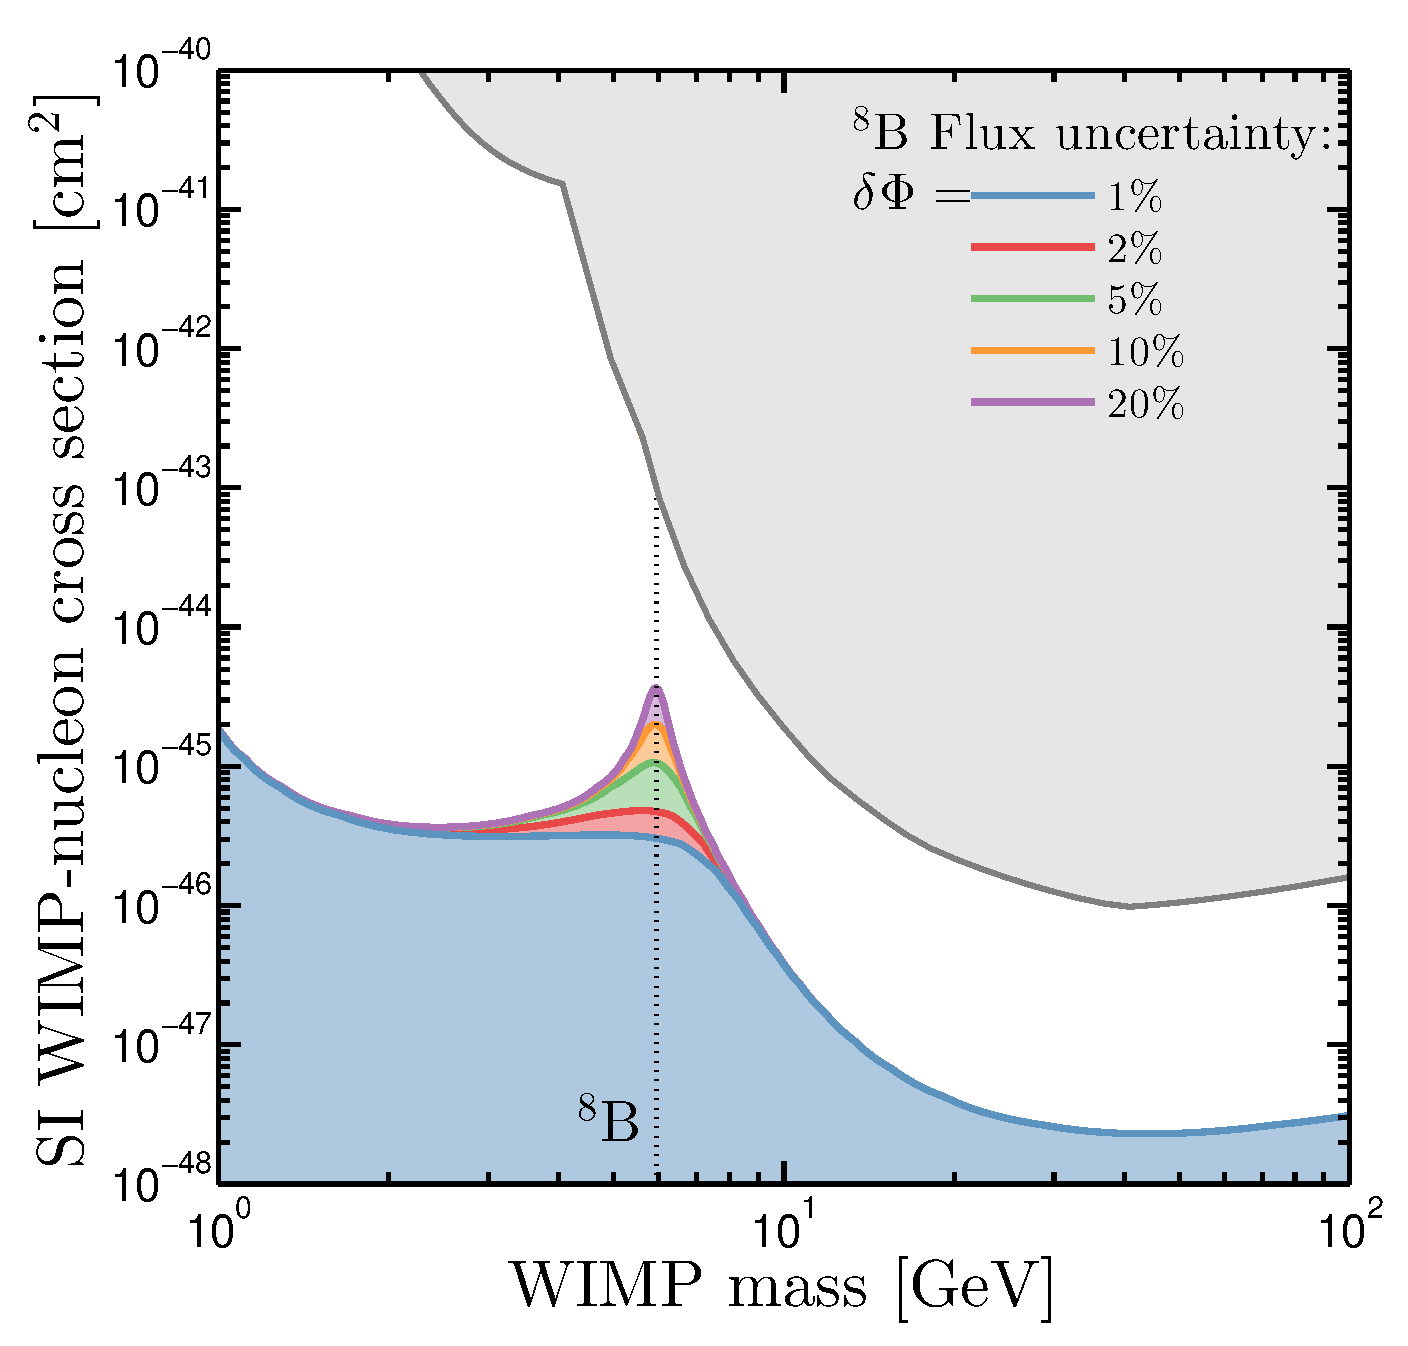
\includegraphics[trim = 0mm 0 0mm 0mm, clip, width=0.48\textwidth,angle=0]{Figures/nufloor_fluxerrs.eps}
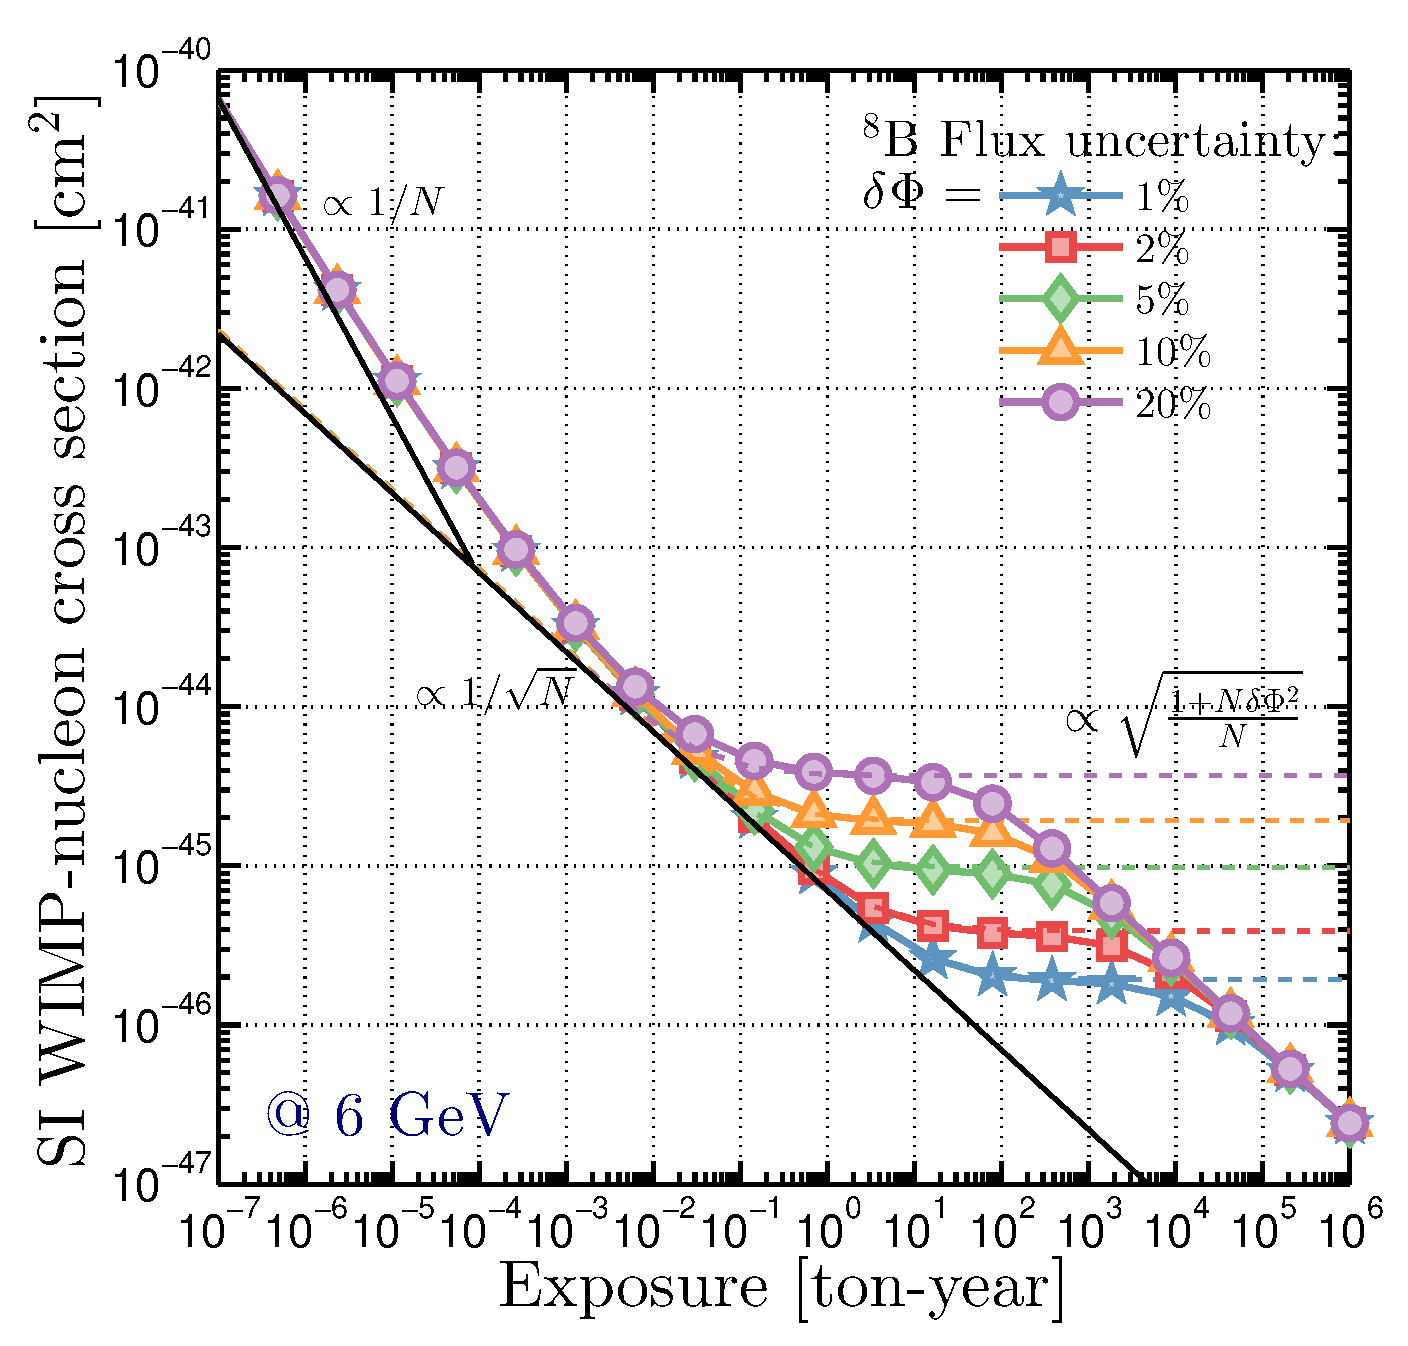
\includegraphics[trim = 0mm 0 0mm 0mm, clip, width=0.48\textwidth,angle=0]{Figures/nufloor_fluxerrsex.eps}
\caption[Effect of the flux uncertainty on the neutrino floor]{SI xenon neutrino floor as a function the uncertainty on the $^8$B neutrino flux. {\bf Left}: the neutrino floor for a 10 ton-year xenon experiment as a function of WIMP mass for flux uncertainties in the range 1\%~-~20\%. We also show the region currently excluded by experiments in grey. {\bf Right}: the evolution of the neutrino floor {\it at} 6 GeV as a function of detector exposure for the same range of flux uncertainty values. We also indicate the three scaling regimes with number of background events $N$.}
\label{fig:nufluxunc}
\end{center}
\end{figure} 
The shape of the neutrino floor (and in fact the presence of the limit itself) is controlled by the level of uncertainty in the expected CNS signal. In the left hand panel of Fig.~\ref{fig:nufluxunc} we show how the assumption for the uncertainty on the $^8$B flux affects the height of the neutrino floor in cross section: for lower uncertainties the neutrino floor appears at lower cross sections, even though the average number of $^8$B events observed in each case is the same. In the right hand panel we show an alternative perspective on the same phenomenon, displaying instead the evolution of the value of the discovery limit at 6 GeV as the exposure of the experiment increases. 

The limits in the right-hand panel of Fig.~\ref{fig:nufluxunc} can be seen evolving through three regimes that we express in terms of the number of background events, $N$. Initially, towards very low exposures the limit approaches a $1/N$ scaling; this is the case for experiments that have less than 1 expected background event over the exposure time. Then as the exposure increases, the limit transitions into a standard Poisson background subtraction regime, scaling as $1/\sqrt{N}$. In experiments with measures to try and distinguish signal from background events, the discovery limit would proceed as $N$ increases in much the same way. However in the presence of neutrinos which mimic the signal, the discovery limit plateaus. The evolution of the discovery limit in this regime is controlled by the systematic uncertainty on the dominant neutrino component according to~\cite{Billard:2013qya},
\be
\sigma_{\rm DL} \propto \sqrt{\frac{1+N\delta \Phi^2}{N}},
\ee
where $\sigma_{\rm DL}$ is the discovery limit and $\delta \Phi$ is the fractional uncertainty on the relevant neutrino flux. In this regime, which persists for $N~\sim 10-1000$, the experiment cannot tell the difference between WIMP and neutrino induced recoils. This saturation of the WIMP sensitivity, spanning over two orders of magnitude in exposure, is what is commonly referred to as the neutrino floor. With statistics at this level the experiment cannot probe WIMP cross sections that induce excesses in the total number of observed events smaller than what could just be attributed to fluctuations within the allowed background uncertainty. For instance, one could imagine a hypothetical situation in which the expected neutrino event rate was known with perfect certainty, in this case there would be no limit to how small a cross section an experiment could probe because, up to Poisson fluctuations, one would know how many events one would need to attribute to neutrino recoils. Unfortunately, in reality we have a finite uncertainty and this will lead to a saturation of any WIMP signal as more neutrino events are seen. It should be noted however that this scaling regime does not continue indefinitely. Eventually the slight differences in the tails of the neutrino and WIMP event rates allow the two spectra to be distinguished once a sufficient number of events have been detected, usually around $\mathcal{O}(1000)$~\cite{Ruppin:2014bra}. Although as can be seen in Fig.~\ref{fig:nufluxunc}, the exposures needed depend on the flux uncertainty.

It is important to keep these uncertainties in mind when projecting future limits because neutrino experiments and Solar model builders are also trying to independently reduce them. For this reason it is likely that the neutrino floor problem will be alleviated somewhat over time as better estimates are made, without any further effort on the part of direct detection experiments. Importantly though this is not a permanent solution, the neutrino floor in this scenario is simply suppressed to lower cross sections. For the remainder of our results we will fix to the current best estimates to the neutrino flux uncertainties as we have already described.

\subsection{Astrophysical uncertainties}\label{sec:nufloor_astro}
\begin{figure}
\begin{center}
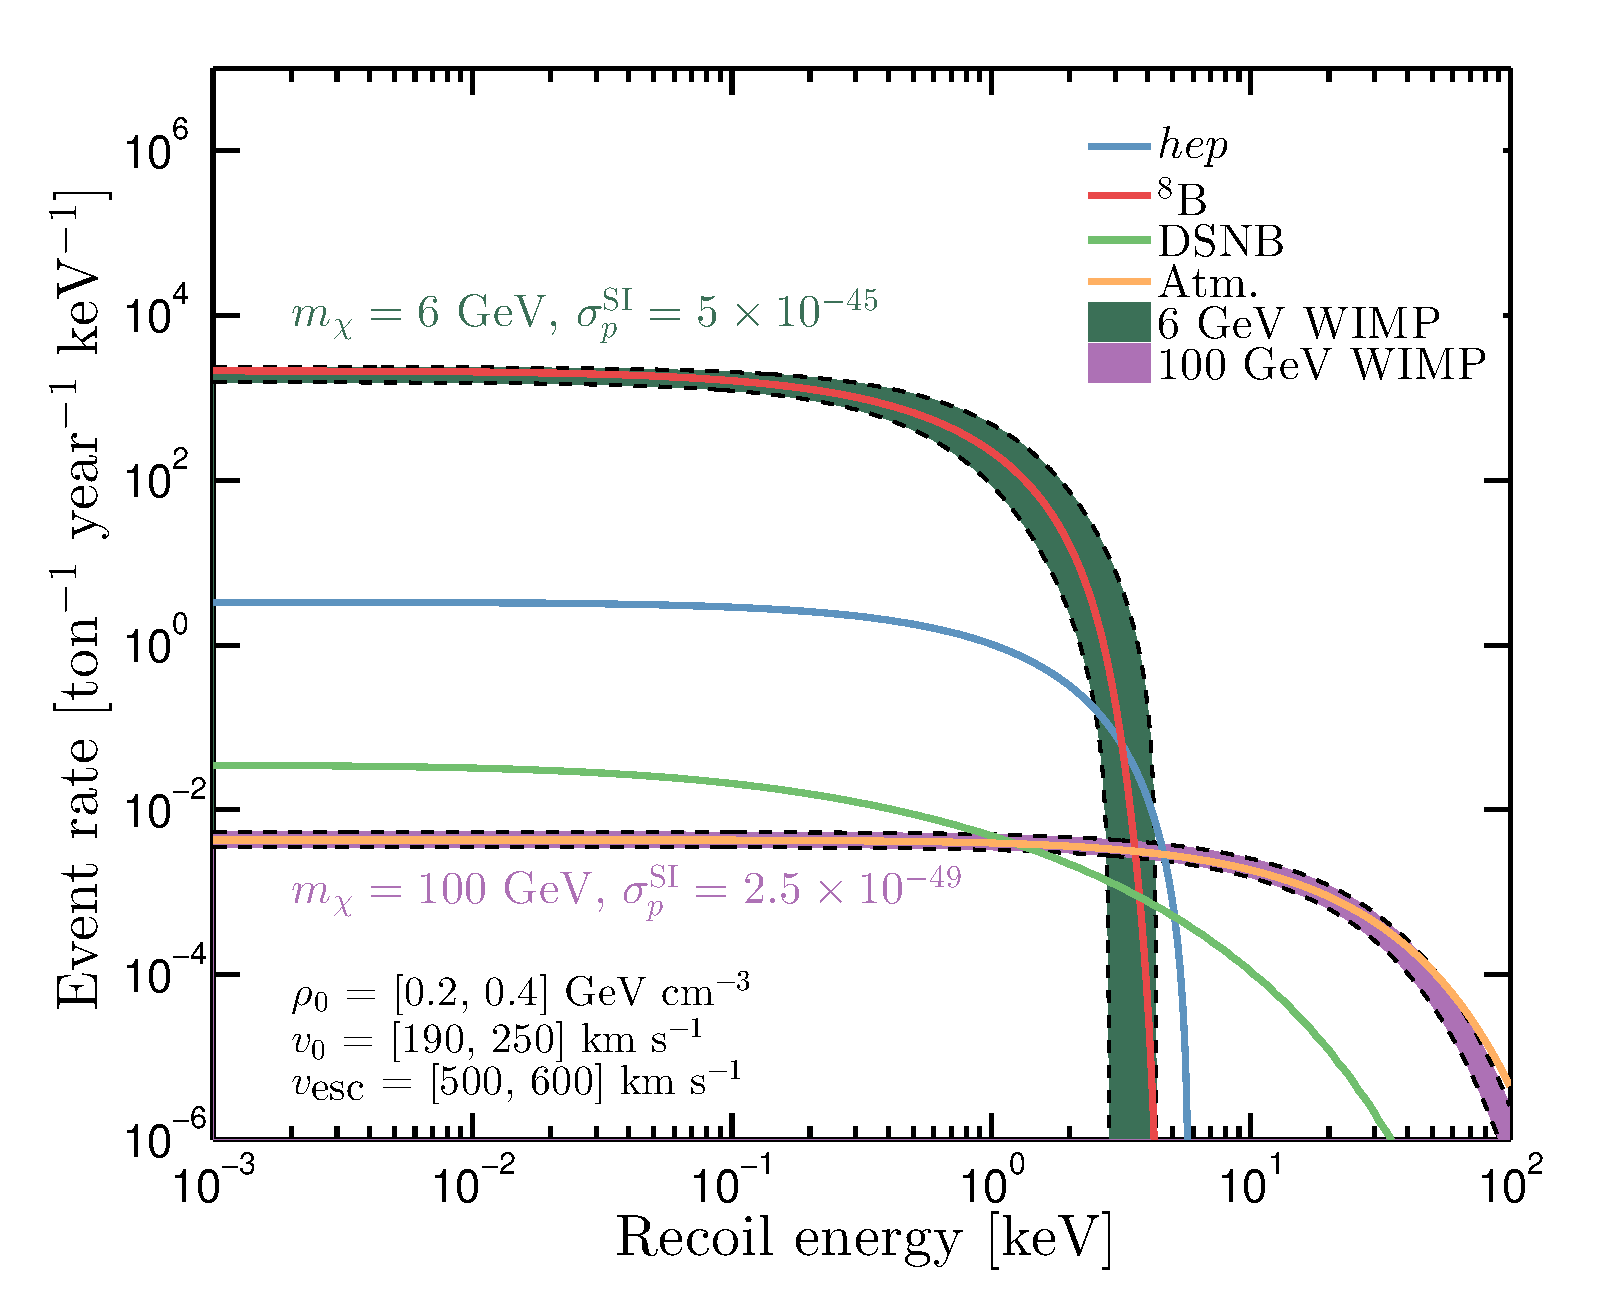
\includegraphics[trim = 0mm 0 0mm 0mm, clip, width=0.8\textwidth,angle=0]{Figures/EventRates_with_uncertainties.eps}
\caption[Effect of astrophysical uncertainties on WIMP recoil spectra]{SI xenon elastic scattering rates for 6 and 100 GeV WIMPs and 4 neutrino sources ($hep$, $^8$B, DSNB and atmospheric neutrinos). The dark green and orange shaded regions respectively refer to the range of scattering rates for 6 and 100 GeV WIMPs with standard halo model parameters taking values between $\rho_0 = [0.2,0.4]$~GeV~cm$^{-3}$, $v_0 = [190,250]$~km~s$^{-1}$ and $\vesc = [500,600]$~km~s$^{-1}$.}
\label{fig:EventRates_with_uncertainties}
\end{center}
\end{figure} 
In addition to sources of uncertainty from the neutrino input we must also consider uncertainties in the WIMP input. We now explain how astrophysical uncertainties influence the shape of the neutrino floor. We focus here on the low mass region. Because light WIMPs probe the tail of the speed distribution, limits in this regime have a greater sensitivity to the values of astrophysical parameters. This choice is also motivated by the fact that advances in technology are more likely to bring about lower threshold detectors (giving access to these low WIMP masses)~\cite{Mirabolfathi:2015pha,Kadribasic:2017obi} than allow exposures in excess of $10^3$ ton-years to be achieved (which are required to reach the neutrino floor due to atmospheric and diffuse supernovae neutrinos).

Figure~\ref{fig:EventRates_with_uncertainties} shows the energy dependence of the nuclear recoil event rate over a range of input values for three free parameters: local density $\rho_0$, circular rotation speed $v_0$ and escape velocity $\vesc$. As mentioned in Sec~\ref{sec:nufloor_nufloor} we see that light WIMPs have a greater sensitivity to changes in the astrophysical input than heavier WIMPs and that the most visible change is around the tail of the recoil distribution (around 1 keV for a 6 GeV WIMP for example). We first discuss the effect of each parameter individually, before embedding the uncertainties in the calculation of the neutrino floor itself.

\begin{figure}
\begin{center}
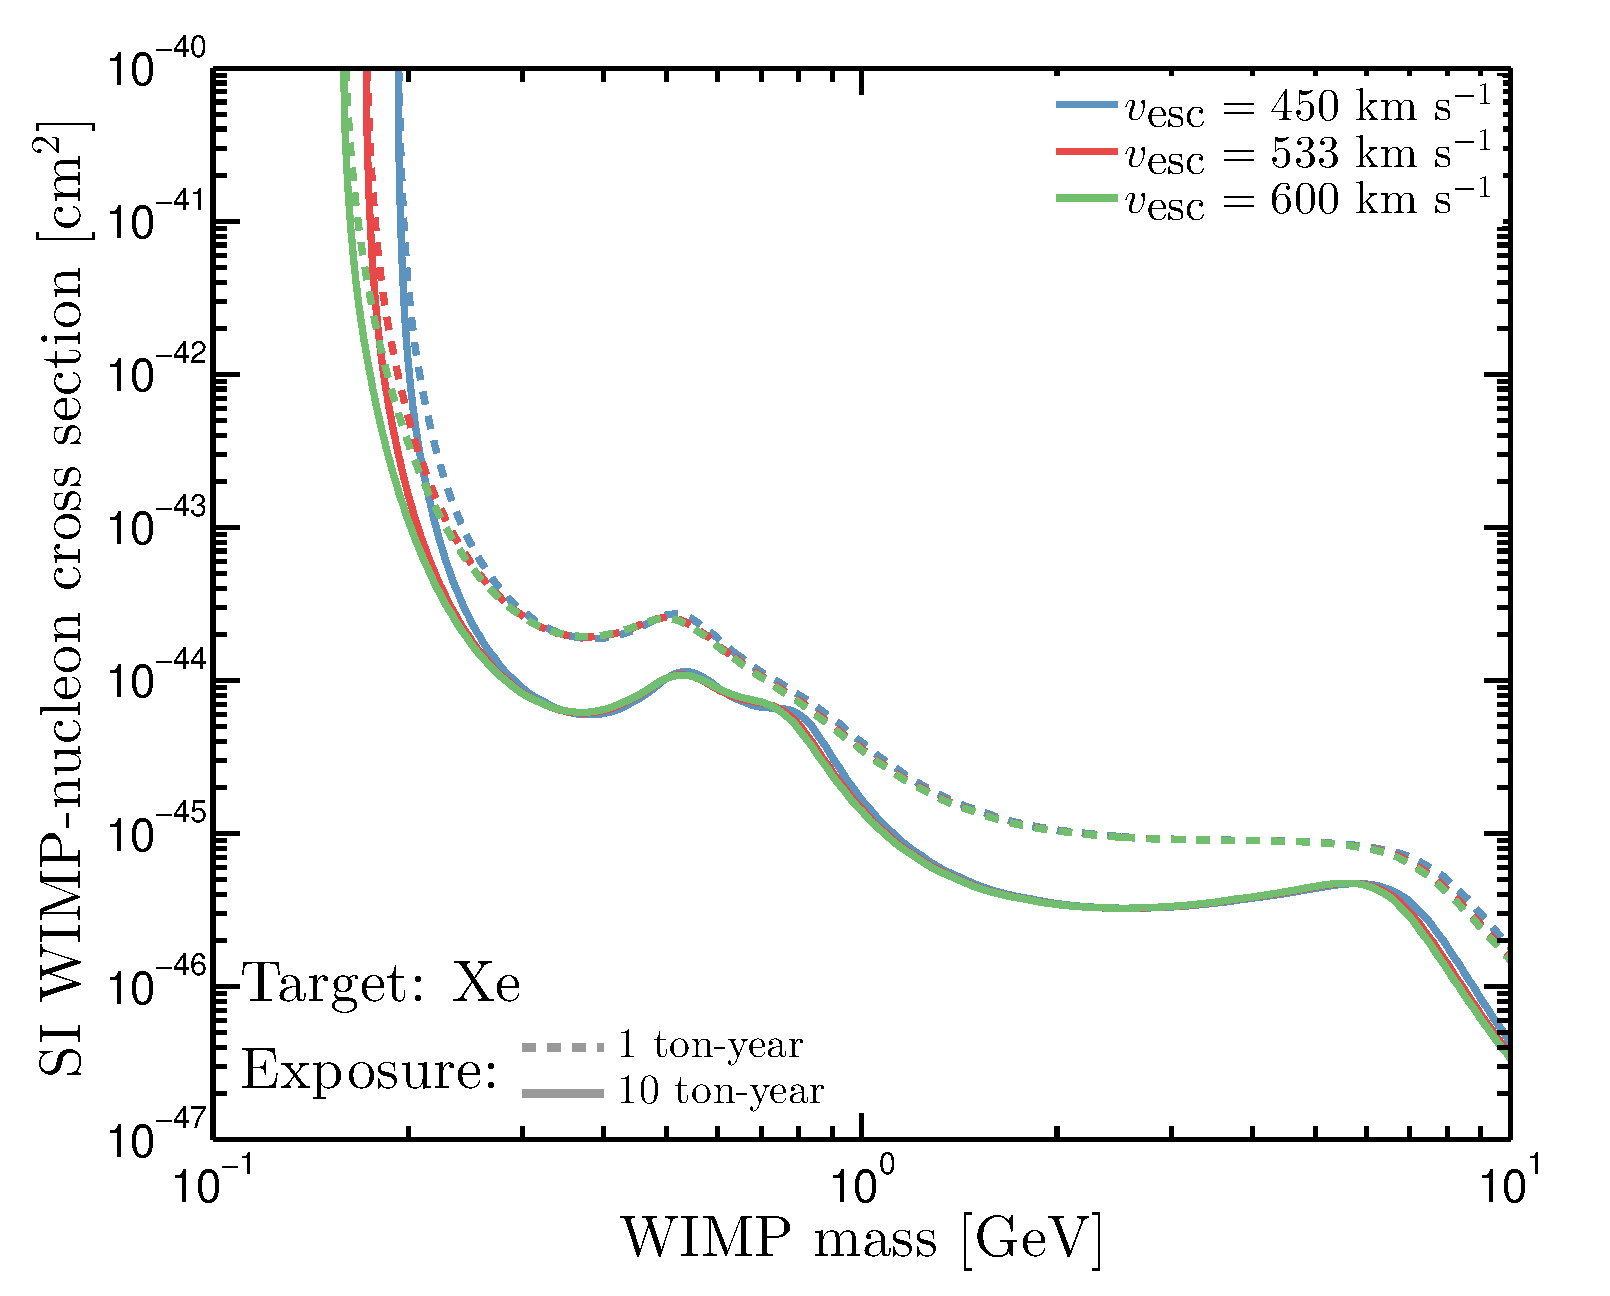
\includegraphics[trim = 0mm 0 0mm 0mm, clip, width=0.8\textwidth,angle=0]{Figures/DL_vesc.eps}
\caption[Neutrino floor with different values of input escape velocity]{SI neutrino floor for a xenon experiment with different values of input escape velocity. The dashed lines are for a 1 ton-year exposure and the solid lines for a 10 ton-year exposure. The blue, red and green colours correspond to input escape velocities of 450, 533 and 600~km~s$^{-1}$ respectively.}
\label{fig:DL_vesc}
\end{center}
\end{figure} 
{\bf The escape velocity} in principle sets the maximum WIMP speed that can be detected on Earth. Since the escape velocity can only control the tail of the recoil distribution and because the speed distribution is very small at its tail, the effect of changing the speed at which it is truncated only has a small impact on the overall shape of the recoil energy spectrum. Figure~\ref{fig:DL_vesc} shows the neutrino floor for 3 values of the escape velocity demonstrating only very marginal differences in the overall shape. The most noticeable effect is around 0.2 GeV where the limits sharply increase due to the maximum energy recoils falling below 3 eV. This is not strictly a feature of the neutrino floor but an artifact of the calculation being performed with a finite cutoff. Apart from some very slight differences in the floors around 0.8 GeV and 8 GeV they are largely indistinguishable. It should be noted that the values of escape velocity chosen in Fig.~\ref{fig:DL_vesc} cover a wider range than the quoted systematic uncertainty in the observed RAVE value of 533 km s$^{-1}$~\cite{Piffl:2013mla}. We deduce that including the uncertainty on $\vesc$ will only have a small effect.




\begin{figure}
\begin{center}
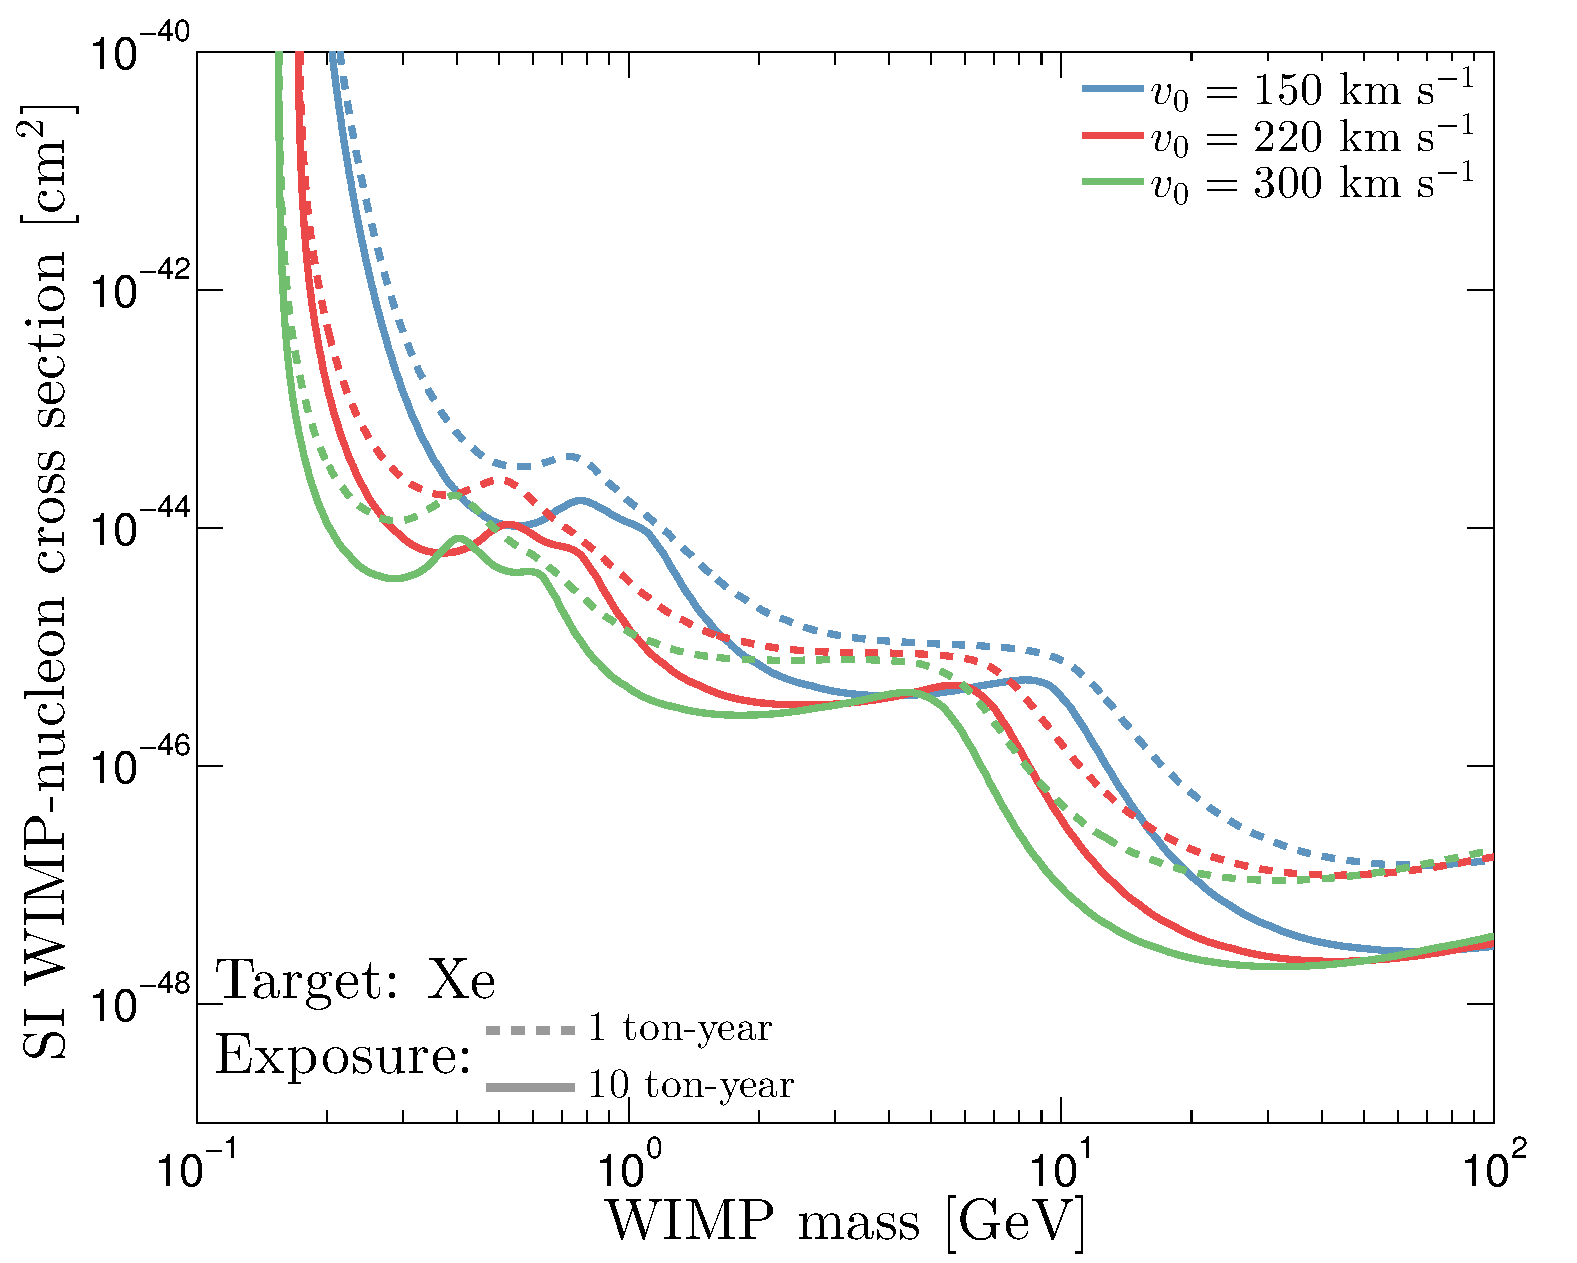
\includegraphics[trim = 0mm 0 0mm 0mm, clip, width=0.8\textwidth,angle=0]{Figures/DL_v0-eps-converted-to.pdf}
\caption[Neutrino floor with different values of input circular velocity $v_0$]{SI neutrino floor for a xenon experiment with different values of input circular velocity $v_0$. The dashed lines are for a 1 ton-year exposure and the solid lines for a 10 ton-year exposure. The blue, red and green colours correspond to an input $v_0$ of 150, 220 and 300 km~s$^{-1}$ respectively.}
\label{fig:DL_v0}
\end{center}
\end{figure} 
{\bf Lab velocity}: The largest source of uncertainty in the laboratory velocity comes from the Sun's circular speed, $v_0$. Given the discrepancies between astronomically observed values for $v_0$, both with each other and with the fiducial value of 220~km~s$^{-1}$~\cite{McMillan:2009yr}, we will be pessimistic about our chosen uncertainty on $v_0$. Figure~\ref{fig:DL_v0} shows the neutrino floor for a range of values of $v_0$. Compared to Fig.~\ref{fig:DL_vesc}, the effect of $v_0$ is much more noticeable. Whereas $\vesc$ influences only the tail of the recoil energy distribution, $v_0$ influences the entirety. For smaller values of $v_0$, larger $m_\chi$ values become mimicked by the same neutrino type, hence the neutrino floor is shifted to higher masses and vice versa.
 
{\bf The local density} appears as a multiplicative factor in the WIMP event rate and as already discussed is degenerate with the scattering cross section. For this study the effect of changing local density is straightforward: a larger value of $\rho_0$ simply shifts the floor to smaller cross sections by the same factor.

\begin{figure}
\begin{center}
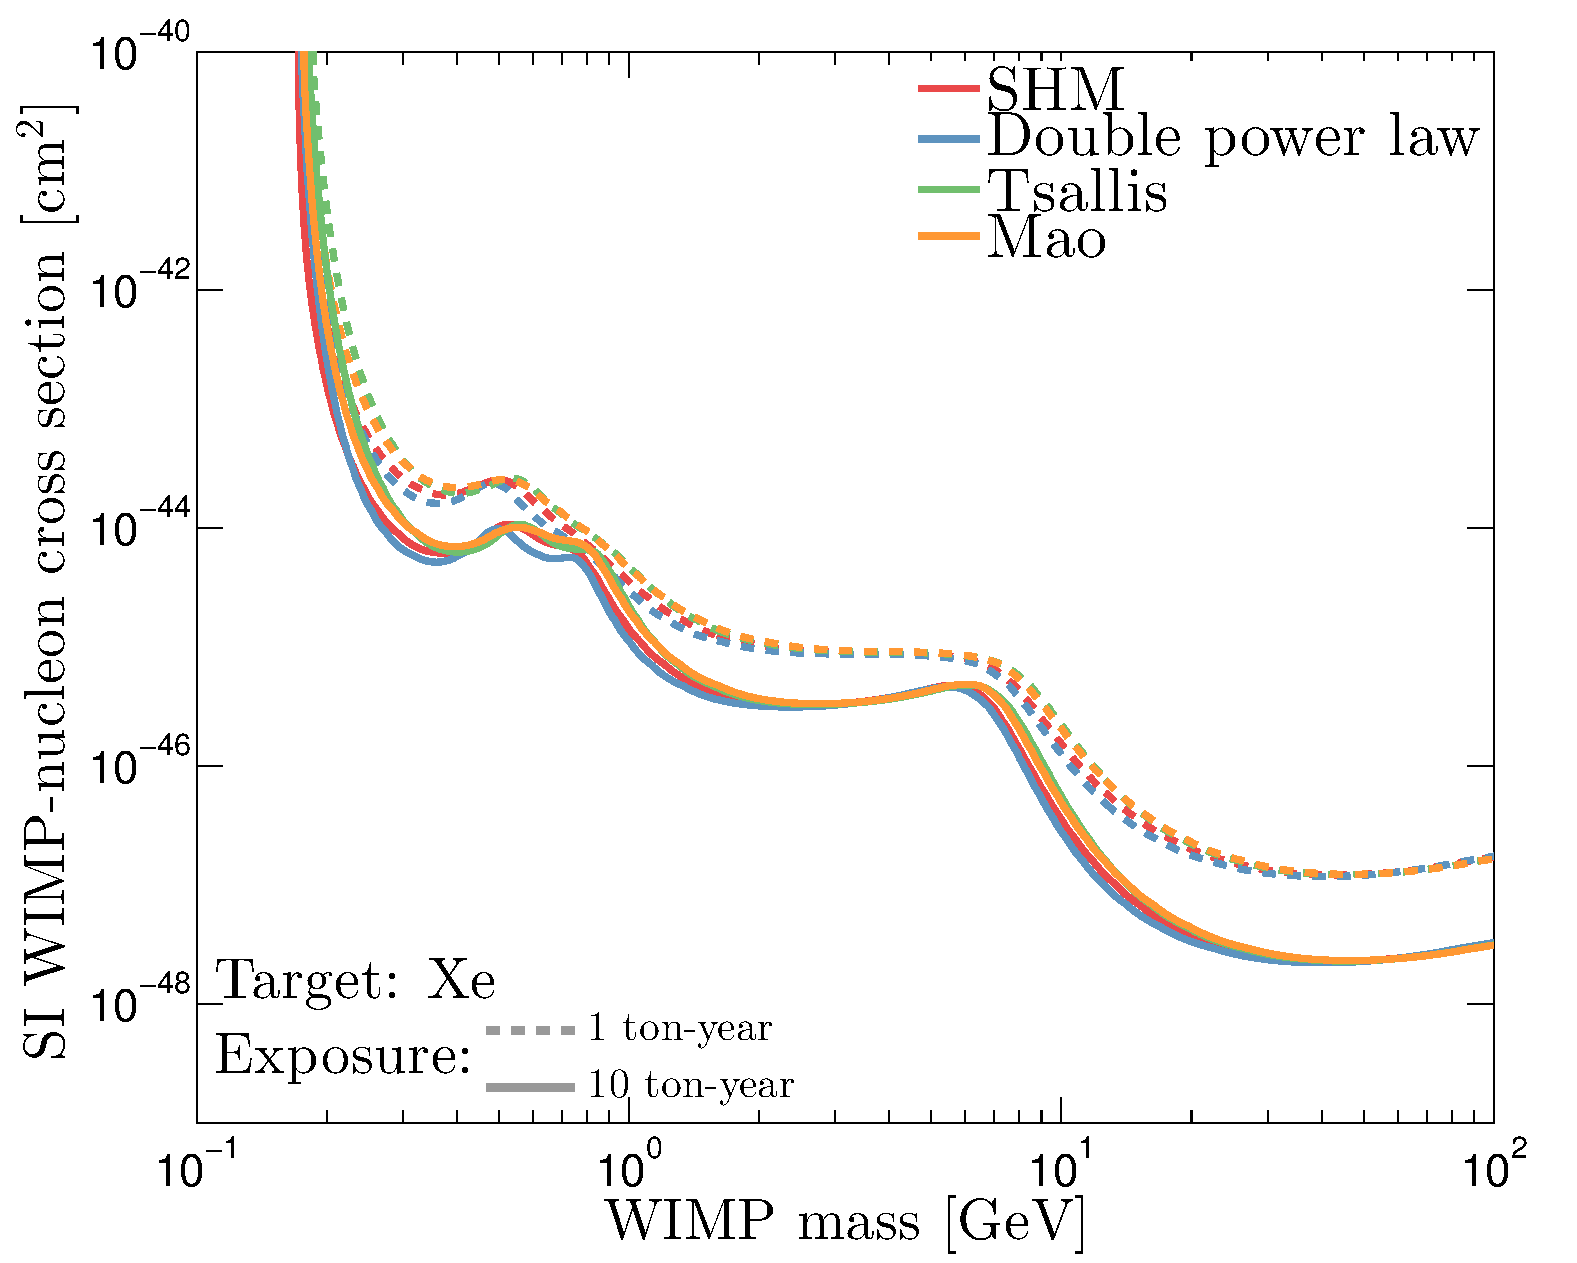
\includegraphics[trim = 0mm 0 0mm 0mm, clip, width=0.8\textwidth,angle=0]{Figures/DL_fv-eps-converted-to.pdf}
\caption[Neutrino floor with different input speed distributions]{SI neutrino floor for a xenon experiment for various input speed distributions. The dashed lines are for a 1 ton-year exposure and the solid lines for a 10 ton-year exposure. The blue, green and orange colours correspond to the double power law, Tsallis and Mao distributions respectively. The red lines are for the SHM with $v_0 = 220$~km~s$^{-1}$ and $v_\textrm{esc} = 533$~km~s$^{-1}$.}
\label{fig:DL_fv}
\end{center}
\end{figure} 
{\bf Speed distribution}: The neutrino floors for alternative speed distributions are shown in Fig.~\ref{fig:DL_fv}. These alternatives, the `double power law', `Tsallis' and `Mao' distributions are outlined in full in Appendix~\ref{app:fv}. They are notable for having departures from a Maxwellian shape at high speeds. For distinguishing neutrinos and WIMPs the high energy tail is important hence we expect that this may induce changes to the shape of the floor. However when we input different underlying speed distributions the position of the floor is altered only very slightly; shifting to slightly higher WIMP masses for the double power law and Mao models and to slightly smaller masses for the Tsallis model. For this reason, and in the interest of efficiency, from here we focus our attention on the SHM. 

\begin{figure}
\begin{center}
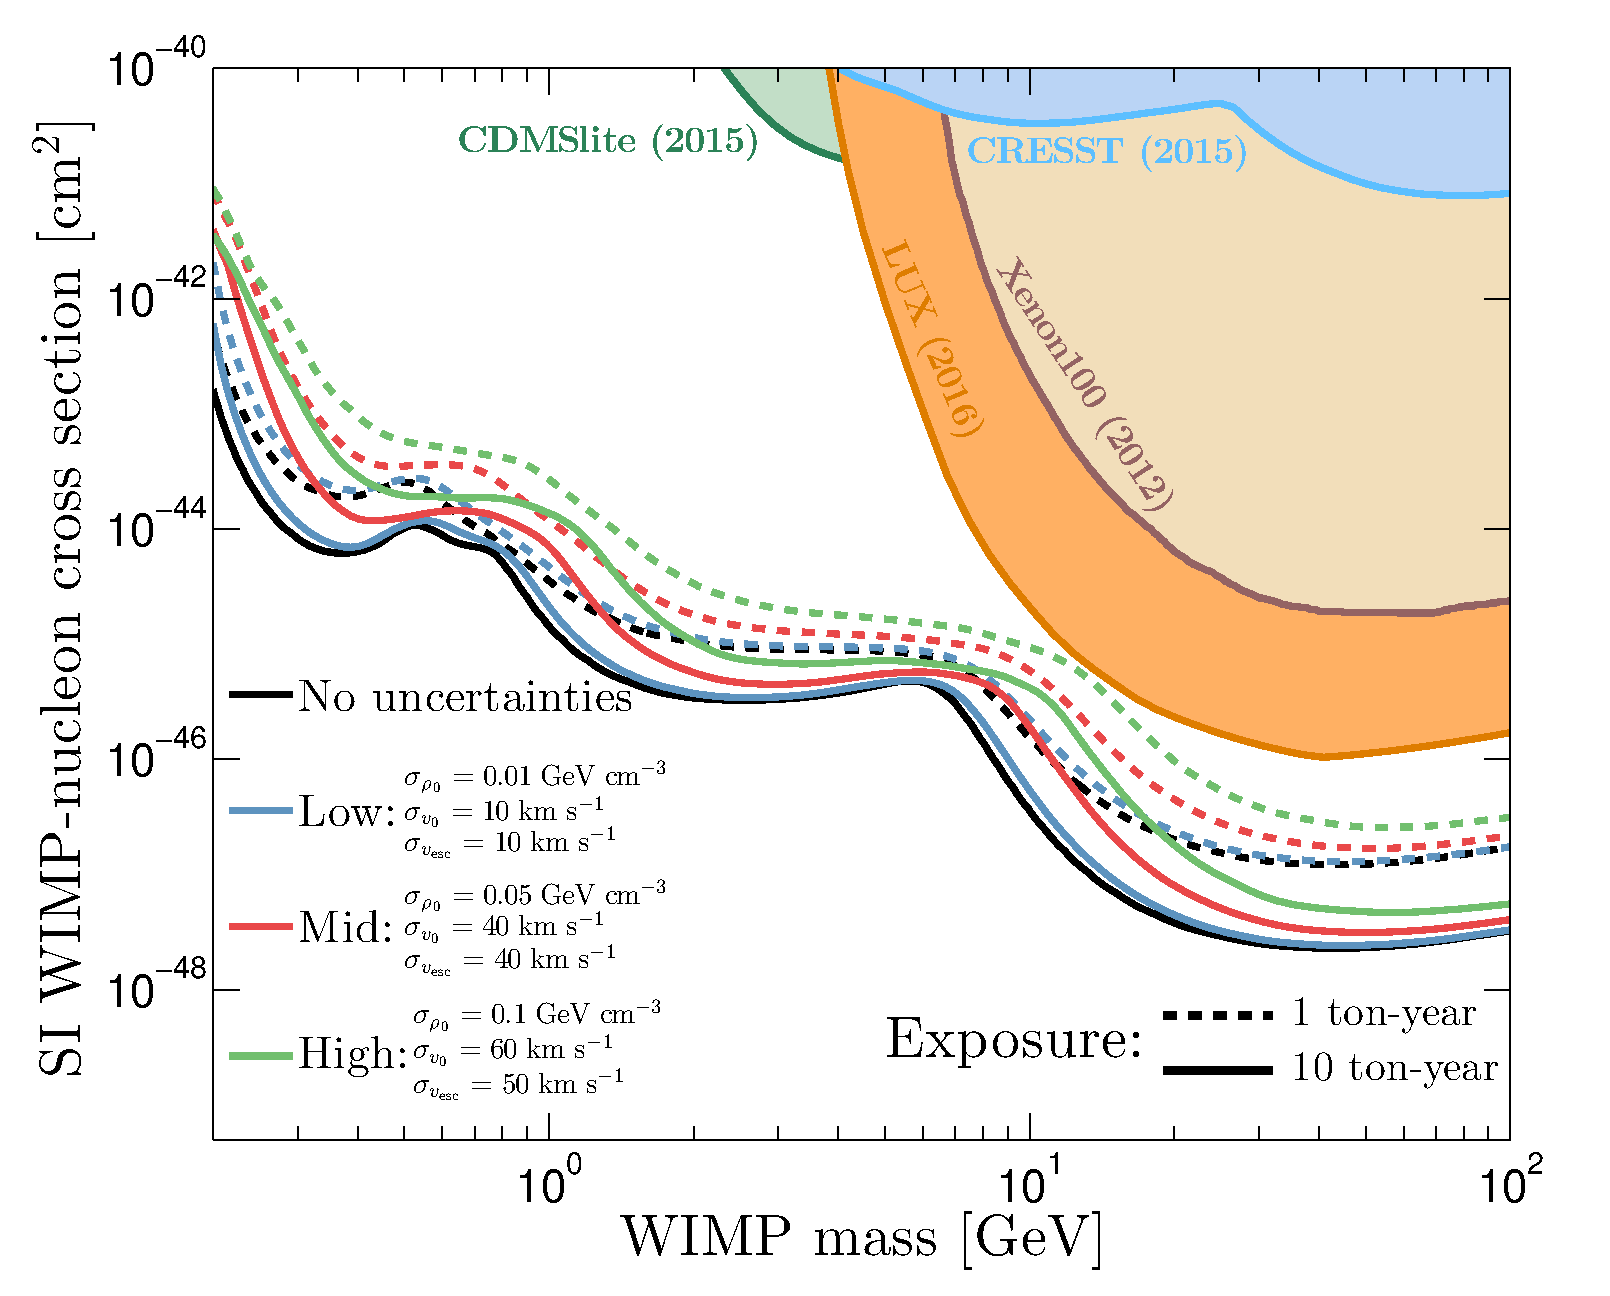
\includegraphics[trim = 0mm 0 0mm 0mm, clip, width=0.8\textwidth,angle=0]{Figures/DL_Uncertainties.eps}
\caption[Neutrino floor with the inclusion of astrophysical uncertainties]{SI neutrino floor as a function of WIMP mass calculated with the inclusion of astrophysical uncertainties in the profile likelihood ratio analysis. The dashed lines are for an exposure of 1 ton-year and the solid lines are with an exposure of 10 ton-years. The blue, red and green curves correspond to 3 sets of values of the 1$\sigma$ uncertainty on the parameters $\rho_0$, $v_0$ and $\vesc$ displayed on the Figure and in the text. The size of the uncertainties are labelled from low to high with values indicated. The filled regions are excluded by experiments, CRESST~\cite{Angloher:2015ewa}, CDMSlite~\cite{Agnese:2015nto}, Xenon100~\cite{Aprile:2012nq} and LUX~\cite{Akerib:2016vxi}.}
\label{fig:DL_uncertainties}
\end{center}
\end{figure}
Now that we have demonstrated the impact of each parameter individually, we unfix them in the profile likelihood ratio test and account for their uncertainty with a multiplicative Gaussian factor. Figure~\ref{fig:DL_uncertainties} shows the discovery limits as a function of the width of this Gaussian uncertainty. We label the sets of uncertainty values ``low'', ``mid'' and ``high''. The low values for the 1$\sigma$ uncertainty on $\rho_0$, $v_0$ and $\vesc$ are respectively, 0.01~GeV~cm$^{-3}$, 10~km~s$^{-1}$ and 10~km~s$^{-1}$. The mid values are 0.05~GeV~cm$^{-3}$, 40~km~s$^{-1}$ and 40~km~s$^{-1}$. And for the high values we use 0.1~GeV~cm$^{-3}$, 60~km~s$^{-1}$ and 50~km~s$^{-1}$.

With the values of the astrophysical parameters uncertain, the experiment is less powerful. The neutrino floor in these cases appears at larger cross sections because the WIMP signal is statistically saturated with fewer events. We also find that the maxima appearing in the discovery limit due to each neutrino component become broader with the inclusion of uncertainties. As shown in the previous Section, the peak in the discovery limit shifts to WIMP masses with recoil energies more closely matching that of the relevant neutrino. Hence, the larger the uncertainty on $v_0$ and $v_\textrm{esc}$ the broader the peak becomes due to the increased range of WIMP masses with recoil energies overlapping with neutrinos. For instance the peak due to $^8$B neutrinos now extends up to 15 GeV for the largest set of astrophysical uncertainties.

This result shows that it is important for the astrophysical input to the predicted WIMP event rate to be well understood if one wishes to interpret how neutrinos play a role in prohibiting the discoverability of certain regions of the WIMP mass-cross section parameter space. Particularly this will be a concern for the next generation of direct detection experiments which are set to make limits that come very close to those calculated in this work. In fact, as we can see in Fig.~\ref{fig:DL_uncertainties}, the floor for ``high'' values of uncertainty comes extremely close to the LUX limit just above 10 GeV. Hence we can conclude that unless there are improvements in the knowledge of the astrophysics parameters or the uncertainties on the neutrino flux, the neutrino floor will be encountered by direct detection experiments much sooner than previously thought.


\subsection{Future detectors}\label{sec:nufloor_future}
\begin{figure}
\begin{center}
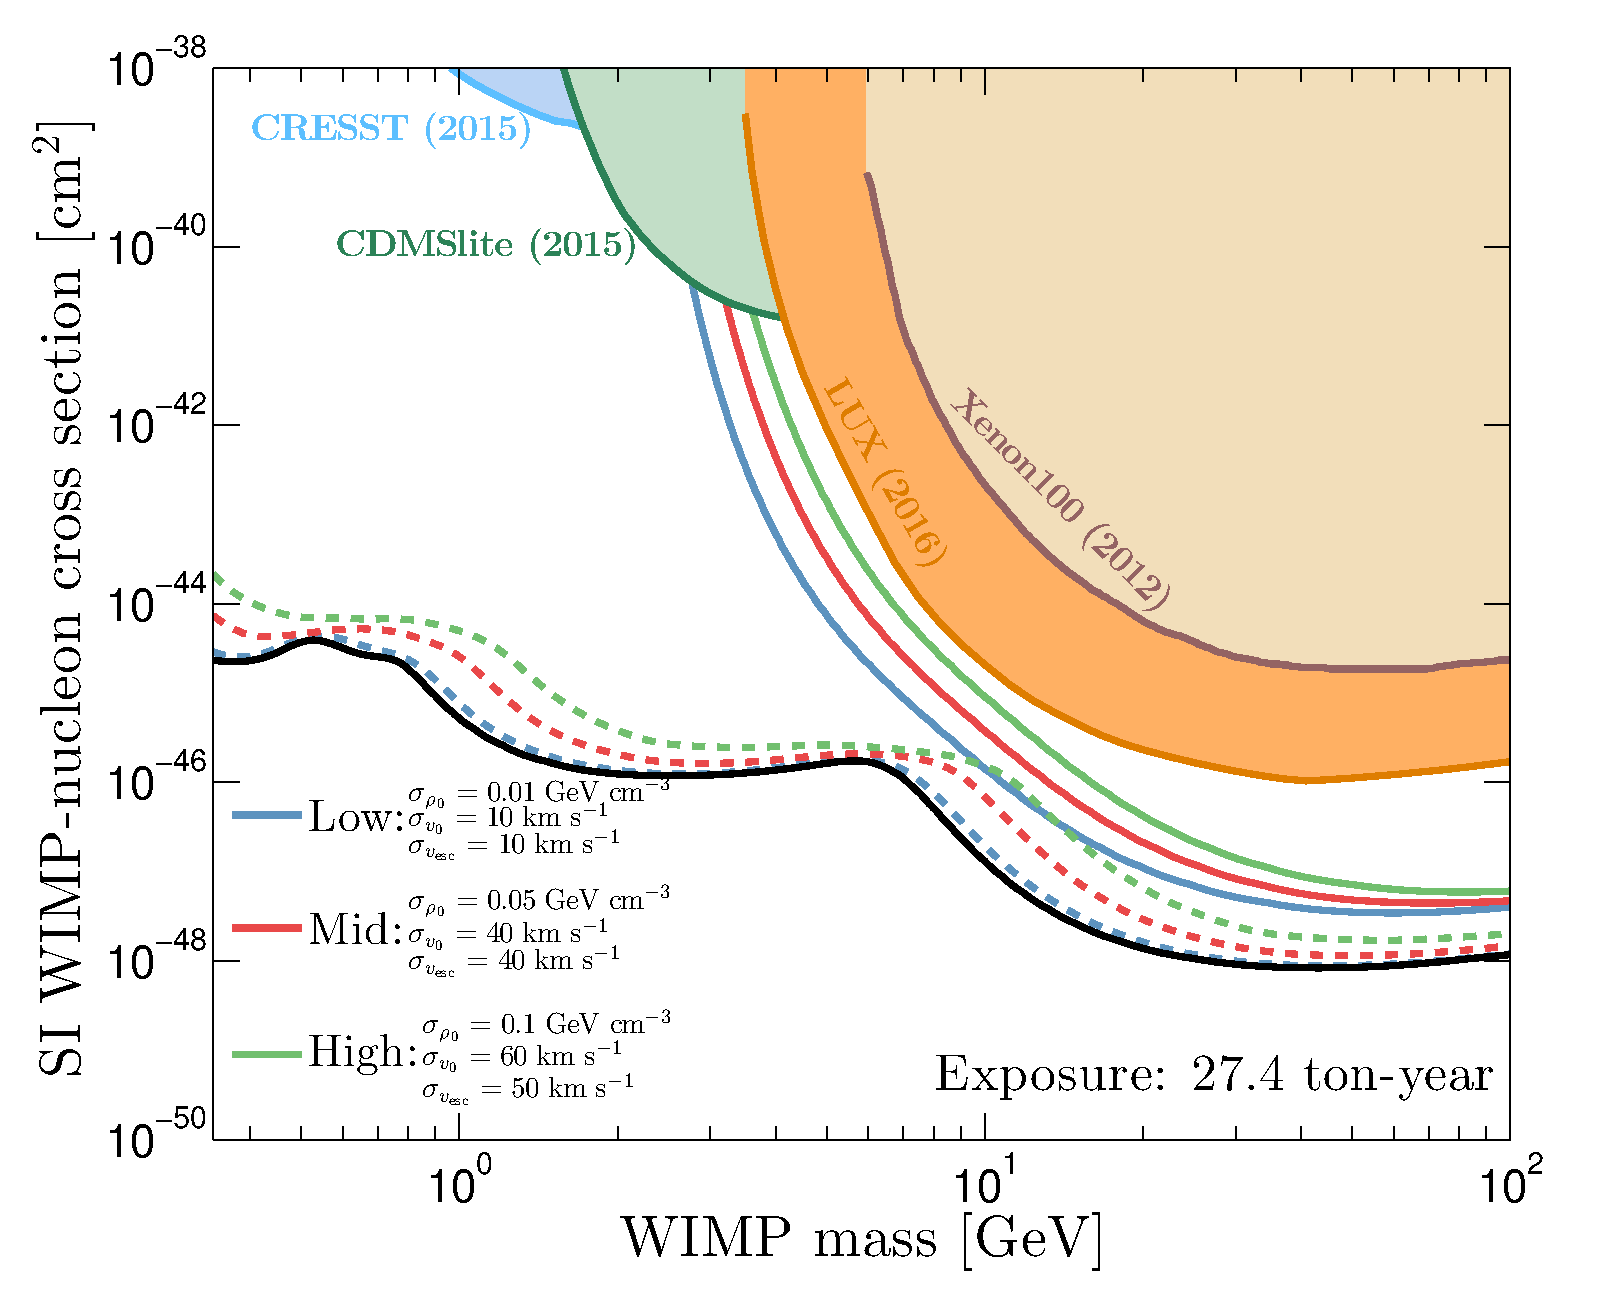
\includegraphics[trim = 0mm 0 0mm 0mm, clip, width=0.8\textwidth,angle=0]{Figures/DL_Resolution.eps}
\caption[Neutrino floor for a realistic detector]{SI discovery limits as a function of WIMP mass for 3 sets of values of the uncertainty placed on the astrophysical parameters: local density, Solar velocity and escape velocity. The blue, red and green curves correspond to low, medium and high values for these uncertainties with 1$\sigma$ values shown. The solid lines are obtained when the detector efficiency is taken into account and the recoil spectrum is convolved with a Gaussian energy resolution with $\sigma(E_r) = 0.8 E_r$ and the corresponding neutrino floors i.e. with no detector effects, are shown as dashed lines. The filled regions are currently excluded by experiments, CRESST~\cite{Angloher:2015ewa}, CDMSlite~\cite{Agnese:2015nto}, Xenon100~\cite{Aprile:2012nq} and LUX~\cite{Akerib:2016vxi}. For comparison we show the neutrino floor calculated without considering astrophysical uncertainties, indicated by the black line.}
\label{fig:DL_Resolution}
\end{center}
\end{figure}
Future direct detection experiments such as Xenon1T~\cite{Aprile:2015uzo} and  LZ~\cite{Akerib:2015cja}, are poised to make the first detection of CNS. So far we have only shown floors that are defined without the consideration of any additional experimental limitations. In practice all detectors suffer from complications such as imperfect energy resolution, efficiency and have thresholds in the $\mathcal{O}(1-10)$ keV range as opposed to the ultra-low thresholds that are used when mapping the low WIMP mass neutrino floor.

We show now discovery limits for a 2 keV threshold xenon detector with a 10 ton target mass over 1000 days running time, a reasonable estimate of the specifications of near future experiments. We include an energy resolution which we take to be 80\% at 1$\sigma$ over the full energy range, i.e. $\sigma(E_r) = 0.8 E_r$. We also take into account the efficiency of the detector which decreases towards the threshold of the experiment. In the following results we assume a simple efficiency curve which increases linearly from 25\% at the threshold energy to 100\% at the maximum energy of 50 keV.

The results of Fig.~\ref{fig:DL_Resolution}, based on this more realistic detector, follow from those of Fig.~\ref{fig:DL_uncertainties}. When the uncertainty on $v_0$ is larger, the floor appears at larger WIMP masses for the same reasons as discussed previously. In this case we see that for the largest uncertainties the discovery limits lie extremely close to existing limits, but have shapes indicating the presence of $\sim$150 $^8$B neutrino events. The inclusion of energy resolution is interesting in this context as it in fact forces some of the neutrino events to be pushed {\it above} the energy threshold of the experiment. However the sensitivity is now also limited by the loss of information due to the smearing of the energy spectrum as well as a reduction in the overall event rate due to the efficiency. So these more realistic limits, despite being subject to a sizable neutrino background, do not yet approach the neutrino floors calculated previously. The general conclusion of Sec.~\ref{sec:nufloor_astro} remains, that larger uncertainty values on the astrophysics content of the WIMP signal weakens the possible constraints that can be made by a future experiment.



\subsection{Parameter constraints}\label{sec:nufloor_parcon}
\begin{figure}
\begin{center}
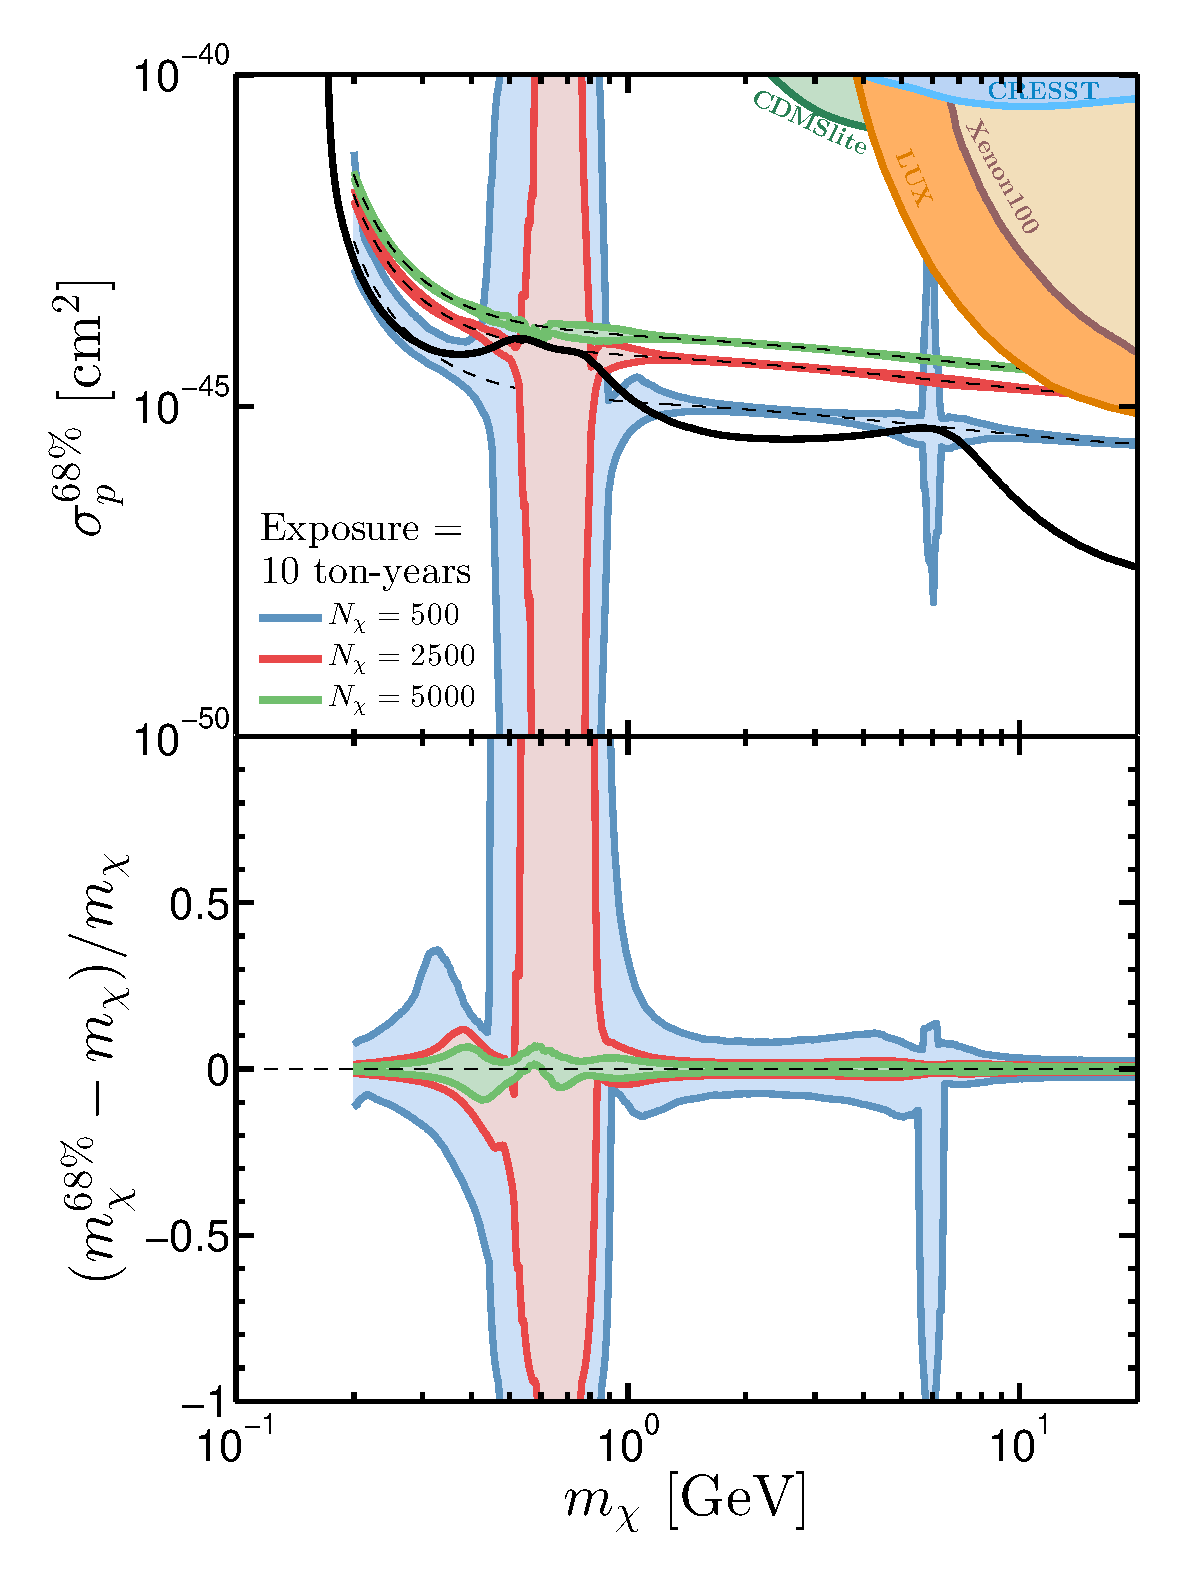
\includegraphics[trim = 5mm 0 0mm 0mm, clip, width=0.49\textwidth,angle=0]{Figures/error_recon.eps}
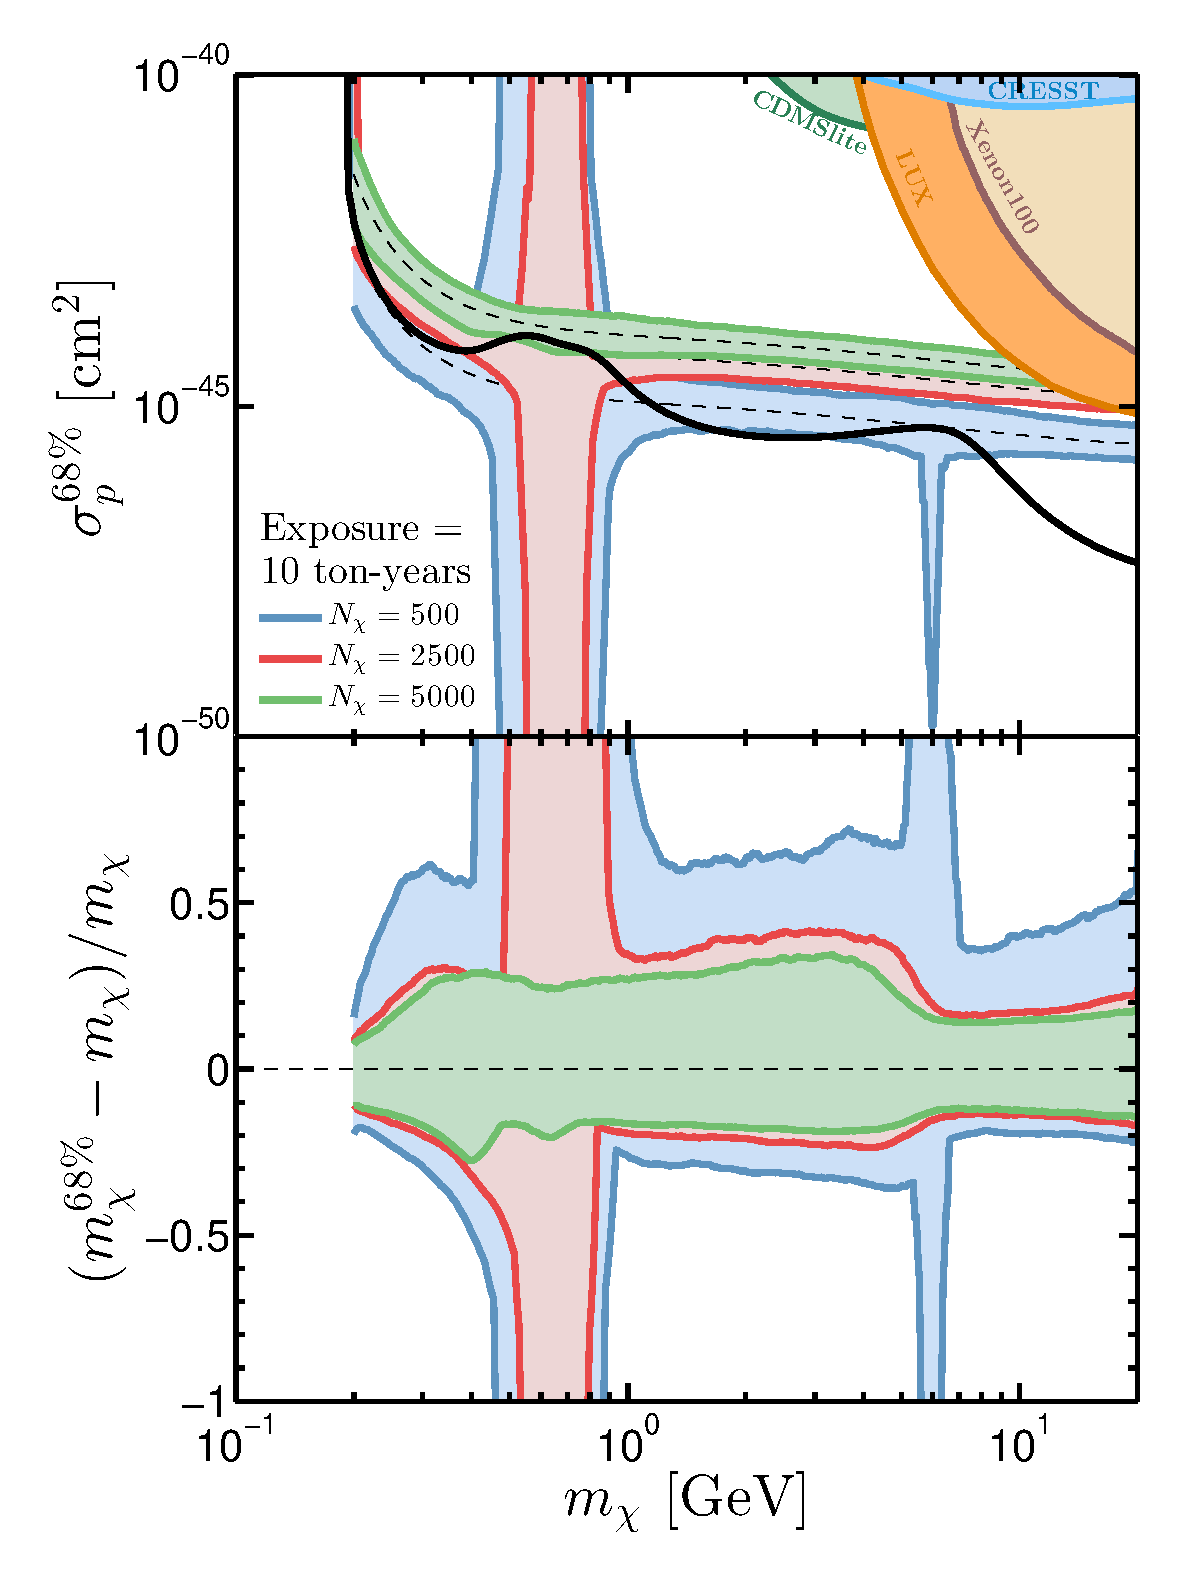
\includegraphics[trim = 5mm 0 0mm 0mm, clip, width=0.49\textwidth,angle=0]{Figures/error_recon_Maxwell.eps}
\caption[Parameters reconstruction under the neutrino background]{{\bf Left:} Reconstructed intervals for $\sigma^{\rm SI}_p$ and $m_\chi$ as a function of input WIMP mass in the presence of the neutrino background. The coloured shaded regions enclose the 68\% confidence intervals on cross section $\sigma^{68\%}_p$ (top panel) and WIMP mass $m^{68\%}_\chi$ (bottom panel, scaled by the input mass $m_\chi$). The input cross section for each WIMP mass is chosen to fix the expected number of WIMP events to 500 (blue), 2500 (red) or 5000 (green). The dashed lines in each region indicate those input values. {\bf Right:} As in the left panel but with $v_0$, $\vesc$ and $\rho_0$ allowed to vary. The filled regions are currently excluded by experiments, CRESST~\cite{Angloher:2015ewa}, CDMSlite~\cite{Agnese:2015nto}, Xenon100~\cite{Aprile:2012nq} and LUX~\cite{Akerib:2016vxi}.}
\label{fig:error_recon}
\end{center}
\end{figure} 
The neutrino floor as derived in the previous section is a convenient way of indicating how much of the WIMP mass-cross section parameter space is accessible to an ideal experiment. However they give us no information with regards to how the ingredient parameters of the WIMP signal may be constrained around this limit, which is undoubtedly a goal of direct detection experiments. To demonstrate this we adopt a similar methodology to the parameter reconstruction introduced in Chapter~\ref{chapter:directional}. We again utilise the nested sampling algorithms provided by {\sc MultiNest}~\cite{Feroz:2007kg,Feroz:2008xx,Feroz:2013hea}, but now exploring the WIMP+neutrino likelihood function, Eq.~(\ref{eq:likelihood}). 

In Fig.~\ref{fig:error_recon} we show the 68\% profile likelihood confidence intervals in the reconstructed values of WIMP mass and cross section, $m^{68\%}_\chi$ and $\sigma^{68\%}_p$. The input values are chosen to produce a fixed number of WIMP events ($N_\chi = 500$, 2500 or 5000 in a 10 ton-year exposure). These lines of constant WIMP event number (shown in Fig.~\ref{fig:error_recon} as dashed lines) are chosen so that they fall either above or below the neutrino floor at various points. For instance the line for $N_\chi= 500$ (green filled region) falls just above the neutrino floor over the full range of WIMP masses, the line corresponding to $N_\chi = 2500$ (red filled region) falls below the floor around 0.6 GeV but above at 6 GeV and the $N_\chi = 5000$ case (blue filled region) falls below the floor around 0.6 GeV and 6 GeV. We can see that input WIMP parameters below the neutrino floor are very poorly reconstructed with 68\% intervals lying outside of the displayed range. However input WIMP parameters above the neutrino floor are reconstructed very well as one would usually expect given the large event numbers. For input values lying on the neutrino floor, for instance at 6 GeV, we see a sharp increase in the error on the reconstructed mass and cross section. 

In the right hand panel of Fig.~\ref{fig:error_recon} we show the results for the same analysis as in the left hand panel but now with the astrophysical parameters unfixed in the likelihood function. For each set of inputs we see a large increase in the recovered intervals across the mass range. We can attribute the increase in error on $\sigma^{\rm SI}_p$ to the additional uncertainty in the expected number of events due to $\rho_0$ and $v_0$. The increase in the $m_\chi$ interval is largely due to the uncertainty on $v_0$ which in particular leads to a huge increase in reconstructed intervals around 6 GeV for the case when $N_\chi = 500$. Following the conclusion of Sec.~\ref{sec:nufloor_astro} which found that accounting for astrophysical uncertainties prohibited a larger range of WIMP parameter values from being accessed, similarly here the inclusion of astrophysical uncertainties has a detrimental effect on the measurement of those parameter values. It is well known that a good understanding of the astrophysics dependence of the WIMP signal is crucial for making measurements of WIMP properties, however this is especially true when neutrinos are the dominant background.

\section{Circumventing the neutrino floor}\label{sec:nufloor_time}
So far we have discussed the phenomenology and shape of the neutrino floor limit itself. Clearly the salient issue is how experiments may search for dark matter in the presence of an ``irreducible'' neutrino background. In other words we want to access cross sections {\it below} the neutrino floor. Perhaps due to the name, the neutrino floor is often misinterpreted as a hard limit to the discoverability of dark matter via direct detection. However the neutrino background is not strictly irreducible. As we described in Sec.~\ref{sec:nufloor_nufluxunc} the `floor' can be conquered with high statistics thanks to the small differences between the WIMP and neutrino recoil spectra. However these high statistics are likely unobtainable by any future experiment so to progress at a more reasonable rate past the neutrino floor we would ideally like to search for some other distinguishing features.

\subsection{Time dependence}
\begin{figure}
\begin{center}
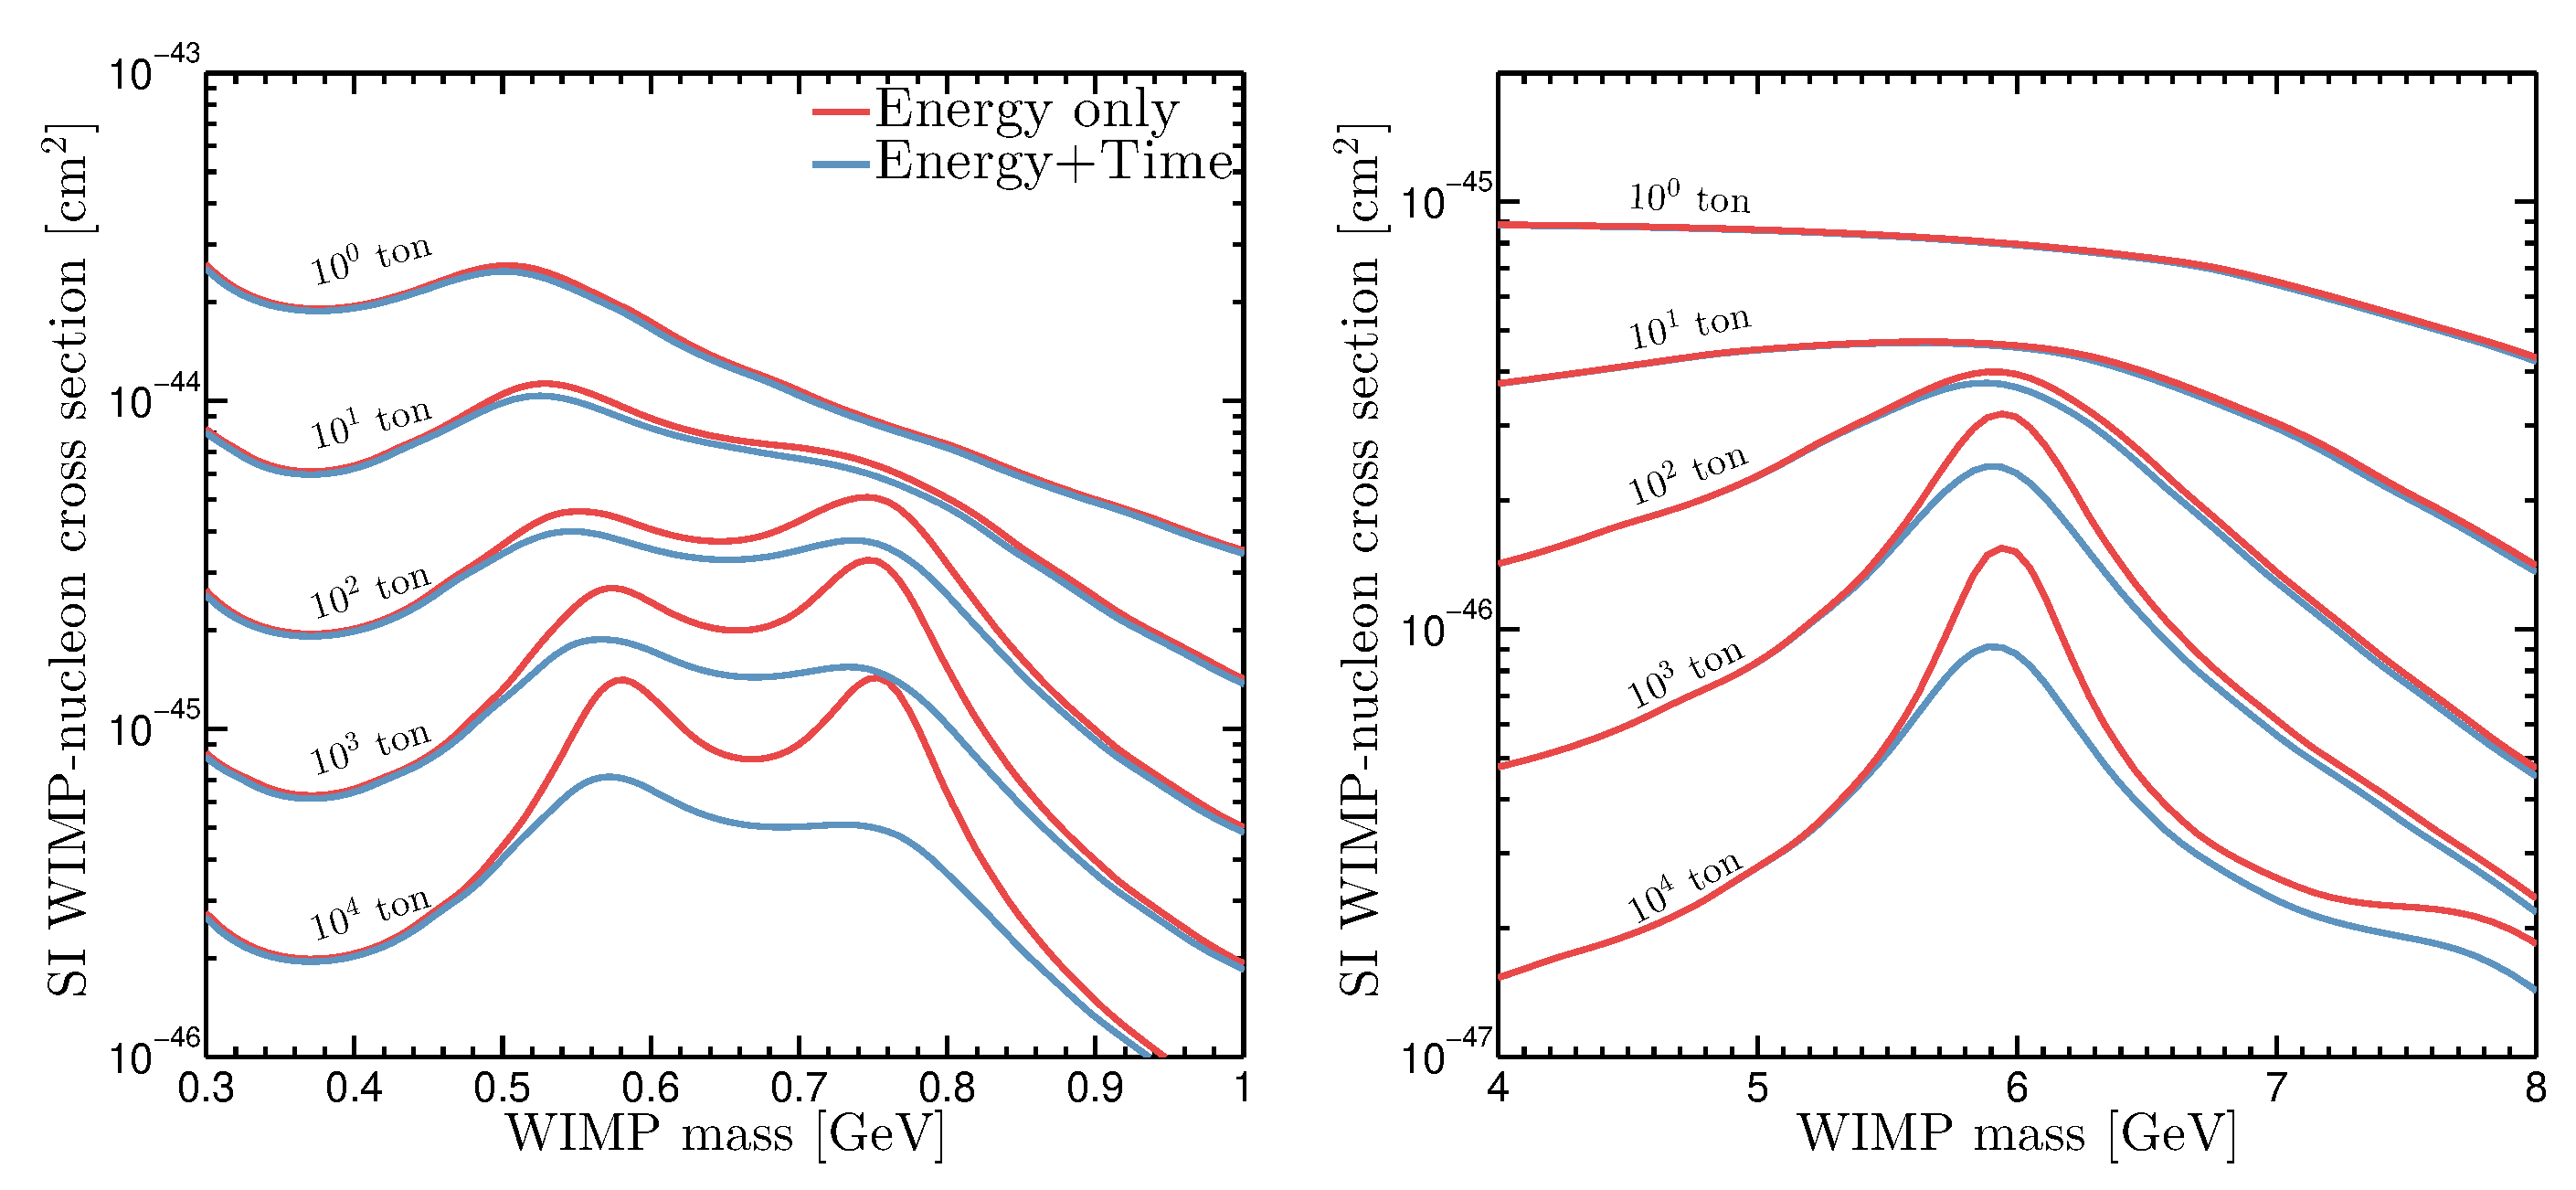
\includegraphics[trim = 0mm 0mm 0mm 0mm, clip,width=\textwidth,angle=0]{Figures/DL_Time.eps}
\caption[Neutrino floor evolution with timing information]{SI neutrino floor evolution in the $0.3 - 1$~GeV ({\bf left}) and $4 - 5$~GeV mass range ({\bf right}). The red curves show the bounds obtained when only energy information is considered and the blue shows the improvement when time information is added. There are four sets of curves shown for detector masses from 1 ton to 10$^4$ tons (top to bottom). In each case the exposure time was kept at a constant 1 year from the 1st of January 2016.} 
\label{fig:DL_Time}
\end{center}
\end{figure}
It was shown in Ref.~\cite{Davis:2014ama} that the time dependence of the WIMP and Solar neutrino event rates provides a distinguishing feature between the two signals which can help circumvent the neutrino floor with fewer events than a recoil energy only analysis. In Fig.~\ref{fig:DL_Time} we show the improvement on the neutrino floor limit after the inclusion of timing information. We show only narrow mass ranges: between 0.3 - 1 GeV when the floor is induced by $^7$Be, $pep$, $^{13}$N, $^{15}$O and $^{17}$F neutrinos and between 4 - 8 GeV due to $^8$B and $hep$ neutrinos. Outside of these specific mass ranges (for the exposures considered here) the improvement offered by time information is negligible. The advantage of including timing information is that in practice, the time tagging of events is often trivial and is common in many experimental configurations. However, because the annual modulation amplitudes are small, obtaining a benefit from time information (over simply not including it) needs in excess of $\mathcal{O}(1000)$ neutrino events. It is clear that to probe further below the neutrino floor we require signals to discriminate between neutrinos and dark matter in a much more pronounced way.




\subsection{Direction dependence}\label{sec:nufloor_res} 
The power of a directional experiment in the context of the neutrino background is fundamentally going to be controlled by the differences in the angular pattern of recoils across the sky\footnote{We do not explore the possibility here, but it may be the case that directional effects can give rise to discrimination between neutrinos and WIMPs in experiments that do not observe recoil tracks, e.g. with spin-polarised $^3$He~\cite{Franarin:2016ppr}.}. The essential aspect that one desires for background rejection is some region of dataspace in which one expects only signal events and no background events. As we have already displayed in Fig.~\ref{fig:Moll} in the full 3-dimensional recoil spectrum such a signal region does exist and is visible by eye. This consideration naturally leads us to contemplate lower dimensional readout scenarios as these will have drastically different angular distributions. Moreover, readout technologies are a principle experimental concern for current directional detection strategies~\cite{Battat:2016pap}. In the following results we will extend beyond the ideal cases of Chapter~\ref{chapter:directional} and consider a range of experimental factors: lower dimensional recoil track projections, head-tail recognition, and finite angular resolution.

We will consider a detector with the $\hat{{\bf x}}$,  $\hat{{\bf y}}$, and $\hat{{\bf z}}$ axes pointing toward the North, the West and the Zenith directions respectively. In the detector frame, the direction of a recoil is given by the angles $\theta$ and $\phi$ defined such that,
\begin{equation}
\hat{{\bf q}} = \sin\theta\cos\phi \, \hat{{\bf x}} + \sin\theta\sin\phi \, \hat{{\bf y}} + \cos\theta \, \hat{{\bf z}} \,.
\label{eq:angles}
\end{equation}

To relate to previous results and the larger literature on the neutrino floor we again focus on a xenon-based experiment. We locate the detector at Modane with latitude and longitude (45.2$^\circ$,~6.67$^\circ$), taking data over a duration $\Delta t = 1$~year. 

For computational efficiency we use now an {\it unbinned} likelihood function,
\begin{equation}
\mathscr{L}(m_\chi,\sigma^{\rm SI}_p,\boldsymbol{\Phi}) = \frac{e^{-(N_\chi+\sum_{j=1}^{n_{\nu}}N^j_\nu)}}  {N_{\rm obs}!} \prod_{i=1}^{ N_{\rm obs}}\left[N_\chi f_\chi(\textbf{d}^i) + \sum_{j=1}^{n_{\nu}}N^j_\nu f^j_\nu(\textbf{d}^i)\right] \prod_{k=1}^{n_{\nu}}\mathscr{L}_k(\Phi_k) \,,
\end{equation}
where the index $i$ runs over the $N_{\rm obs}$ events and the indices $j$ and $k$ relate to the $n_\nu$ neutrino backgrounds. We use $N_\chi$ and $N^j_\nu$ for the expected number of WIMP and neutrino events respectively. We now introduce $f_\chi(\textbf{d}^i)$ and $f_\nu^j(\textbf{d}^i)$ for the WIMP and neutrino event distributions at data point $\textbf{d}^i$ which will have a dimensionality corresponding to the number of observables in the experiment. We compare six strategies:
\begin{itemize} \itemsep0em 
 \item 3-d directional readout, $\textbf{d} = \{E_r,\theta,\phi,t\}$
 \item 2-d directional readout, $\textbf{d} = \{E_r,\phi,t\}$
 \item 1-d directional readout, $\textbf{d} = \{E_r,\theta,t\}$
 \item No directional information $\textbf{d} = \{E_r,t\}$
 \item Event time only $\textbf{d} = \{t\}$
 \item Number of events only (i.e. a counting experiment) $f_\chi = f^j_\nu = 1$
\end{itemize}
The 3-d directional readout, $\{E_r,\theta,\phi,t\}$, corresponds to the optimum detector that measures and exploits all the information available, e.g.~a low pressure gaseous TPC. For a 2-d readout, $\{E_r,\phi,t\}$ only a 2-dimensional ($x$,$y$) projection of the drifted electron cloud can be measured (e.g.~in a CCD readout TPC); and in 1-d, $\{E_r,\theta,t\}$, only a measurement of the projection of the recoil track along the drift ($z$) direction (e.g. with columnar recombination).

The last two strategies we list correspond to detectors that can only measure the total number of events above some threshold. This is the case for bubble chamber experiments~\cite{Cushman:2013zza} that adjust their operating pressure to nucleate a single bubble from a nuclear recoil. Such experiments would have very poor inherent background rejection capabilities, but they are an informative benchmark to consider in this comparative study. The energy and time, $\{E_r,t\}$, strategy corresponds to the majority of current and ongoing direct detection experiments.

\begin{figure}
\begin{center}
%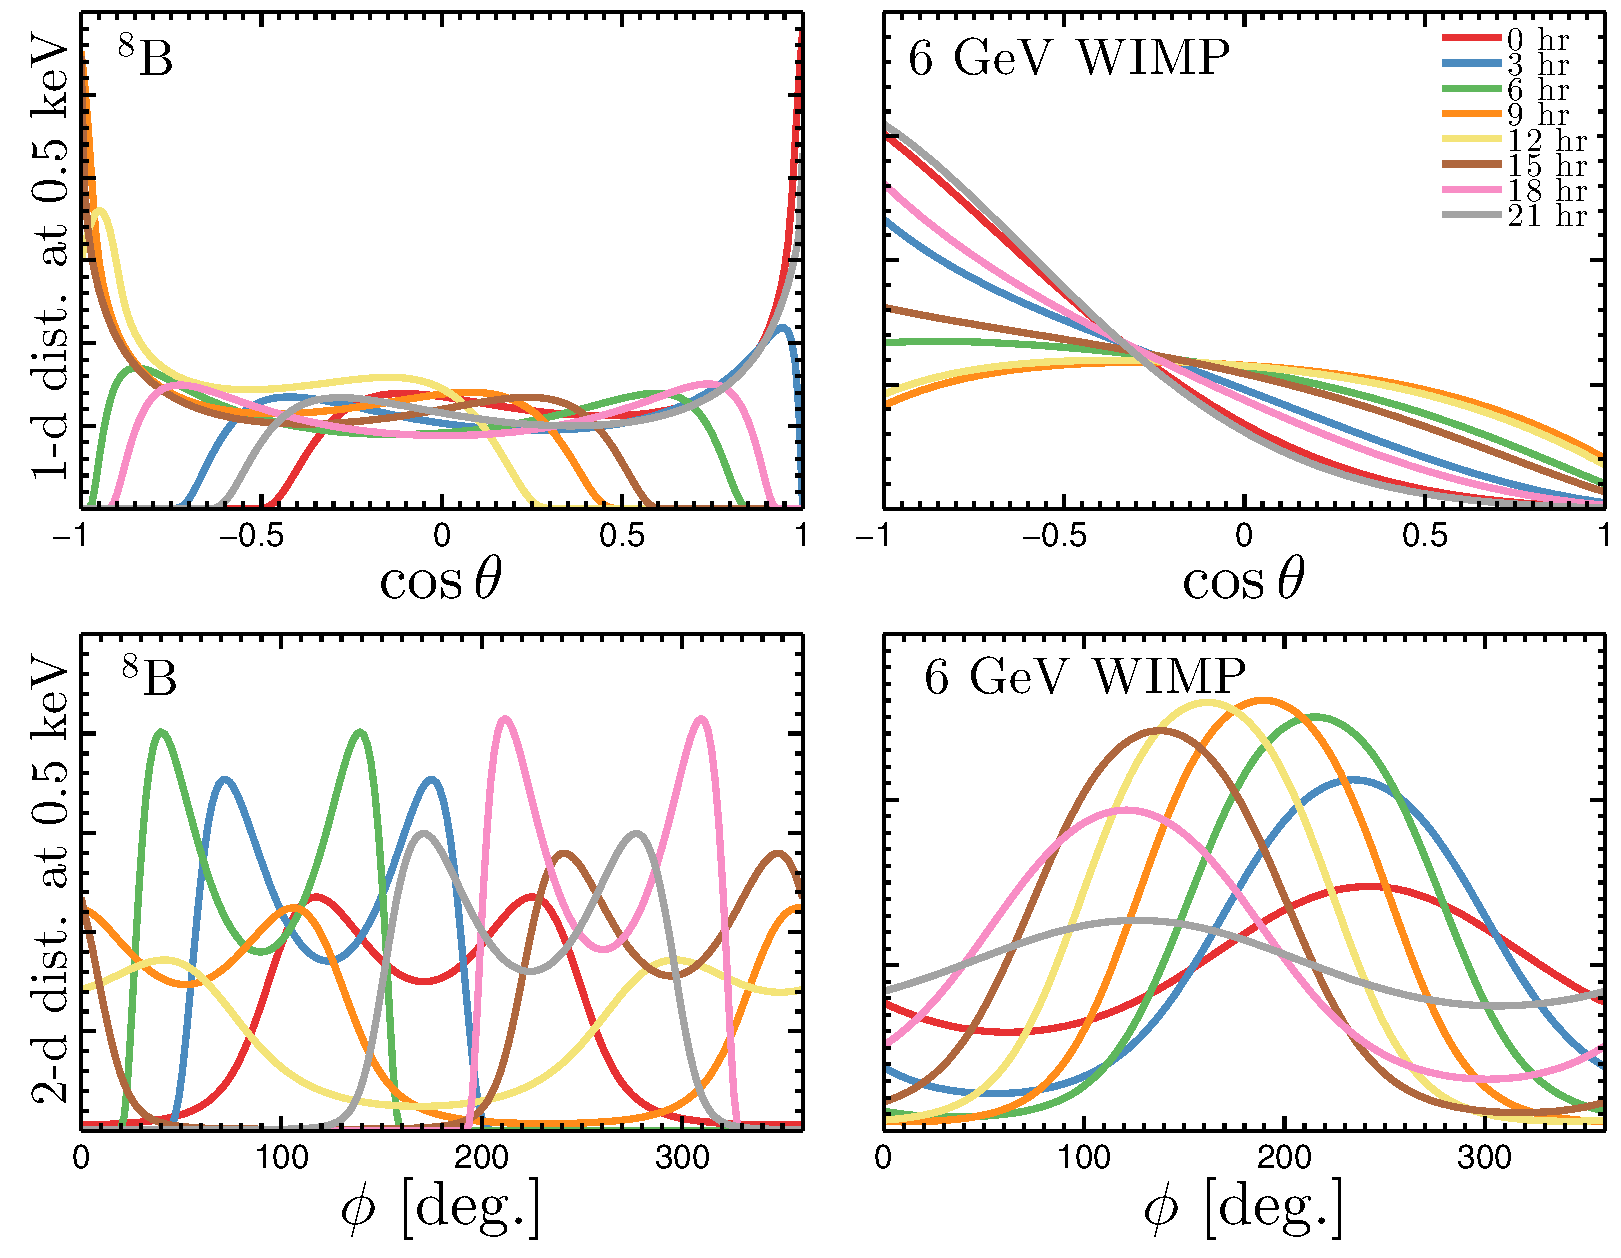
\includegraphics[width=\textwidth,angle=0]{Figures/Daily_1D2D_evolution-eps-converted-to.pdf}
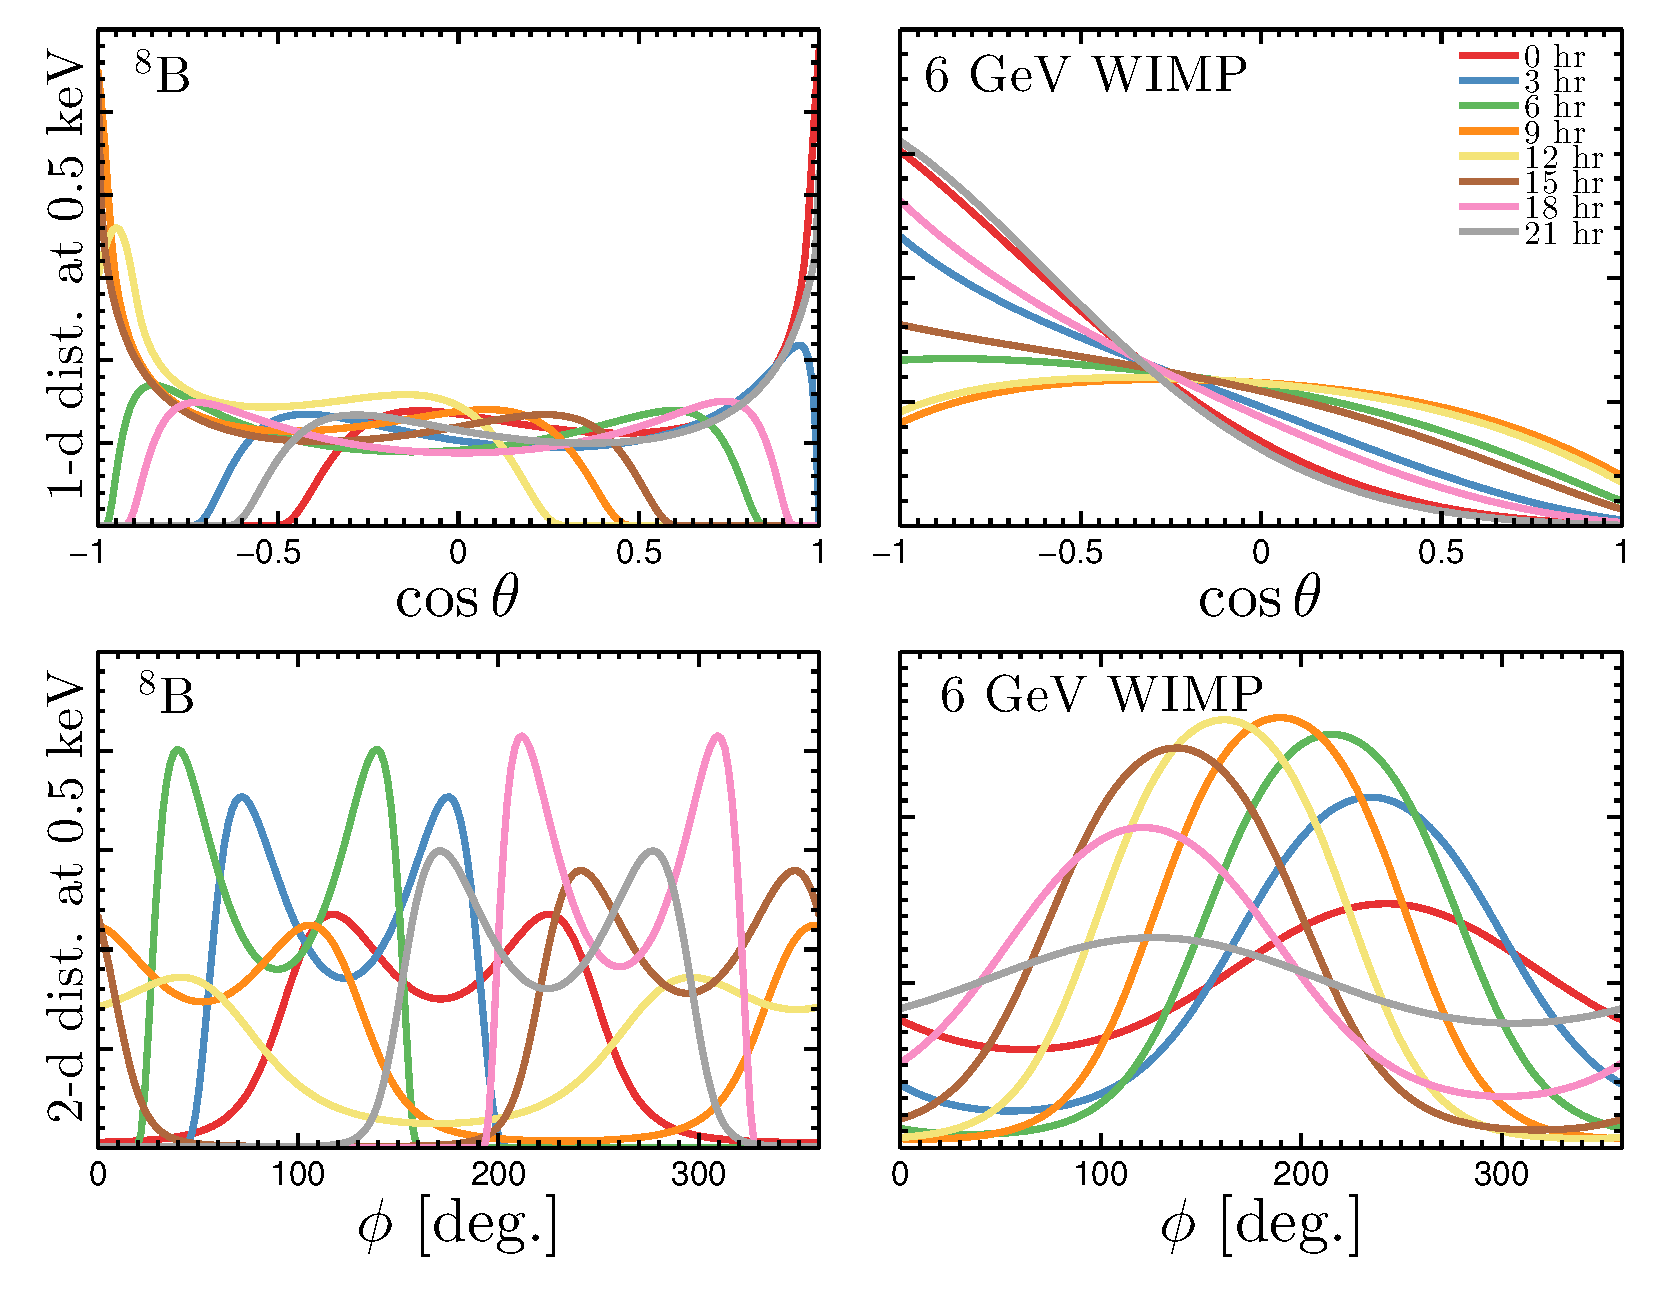
\includegraphics[trim = 0mm 0 0mm 0mm, clip, width=0.99\textwidth]{Figures/Daily_1D2D_evolution.eps}
\caption[Daily evolution of recoils from ${}^{8}\rm{B}$ neutrinos and WIMPs]{The daily evolution, at three hourly intervals, of the angular distributions of 0.5 keV xenon recoils from
${}^{8}\rm{B}$ neutrinos (left column) and a WIMP with mass $m_{\chi} = 6 \, {\rm GeV}$ (right). The distributions are normalised to unity in each case and displayed with arbitrary units. The top row shows the distribution of $\cos{\theta}$  measured by a detector with 1-d readout and the bottom row the angle $\phi$  for  2-d readout. The date chosen was September 6th, when the angular separation between Cygnus and the Sun is maximised.} 
\label{fig:daily1d2d}
\end{center}
\end{figure} 
Figure~\ref{fig:daily1d2d} shows the daily evolution of the 1-d ($\cos{\theta}$), and 2-d ($\phi$), recoil angle distributions at a single energy ($E_r~=~0.5$~keV) from ${}^{8}\rm{B}$ neutrinos and a WIMP with mass $m_{\chi} = 6 \, {\rm GeV}$. The $\phi$ distributions from $^8$B neutrinos have two peaks, because at a fixed recoil energy the neutrino energy spectrum produces recoils in a ring around the incident direction. In the WIMP case, however, the distribution of recoils is peaked in a single direction, towards $-\textbf{v}_\textrm{lab}$. The 2-d and 1-d distributions for both atmospheric and DSNB neutrinos are flat, and therefore we do not show them for clarity. The WIMP and neutrino distributions are significantly different, not only in their shape at a single time but also how they evolve over the course of a day. This suggests that a detector with only 1-d or 2-d readout should still be able to discriminate WIMP and neutrino induced recoils.


\begin{figure}
\begin{center}
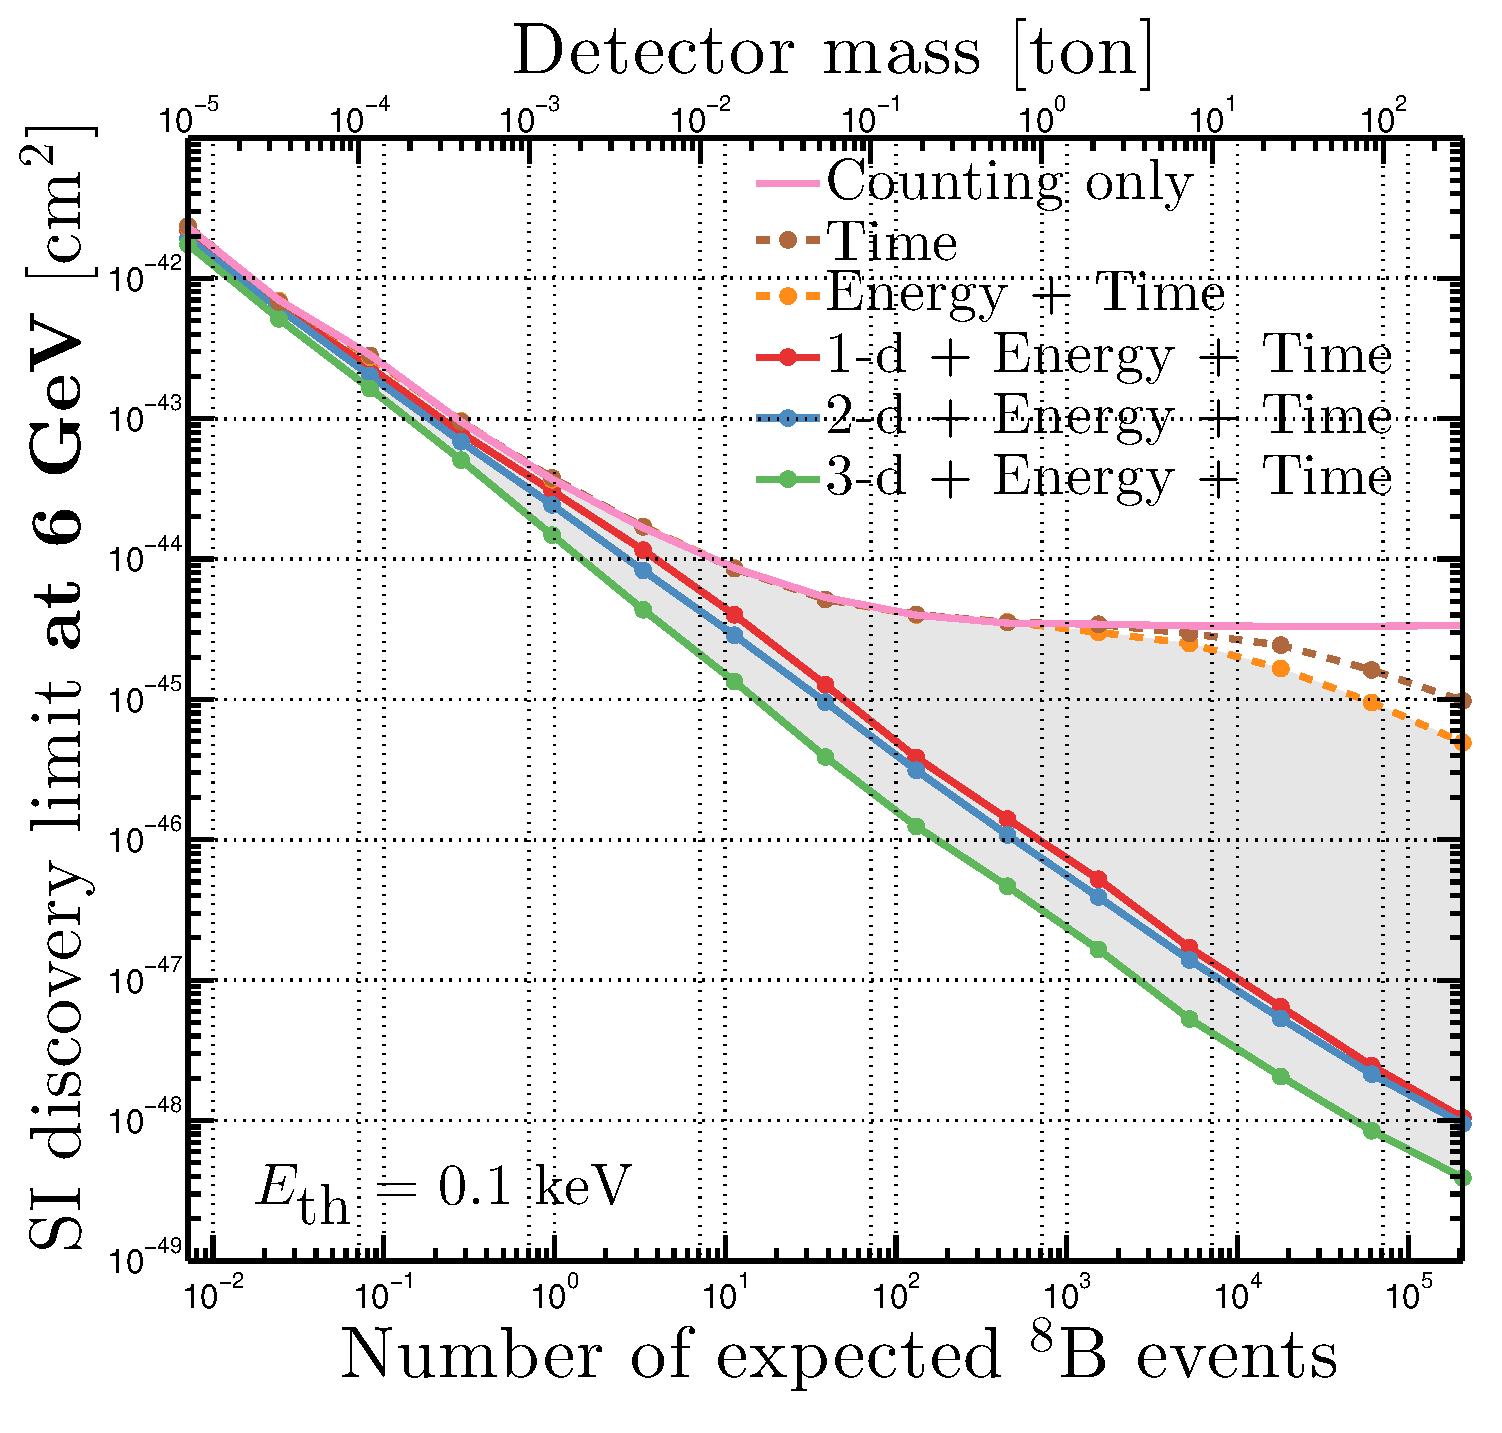
\includegraphics[trim = 0mm 0mm 0mm 0mm, clip,width=0.49\textwidth,angle=0]{Figures/SI_discovery_Xe_6GeV.eps}
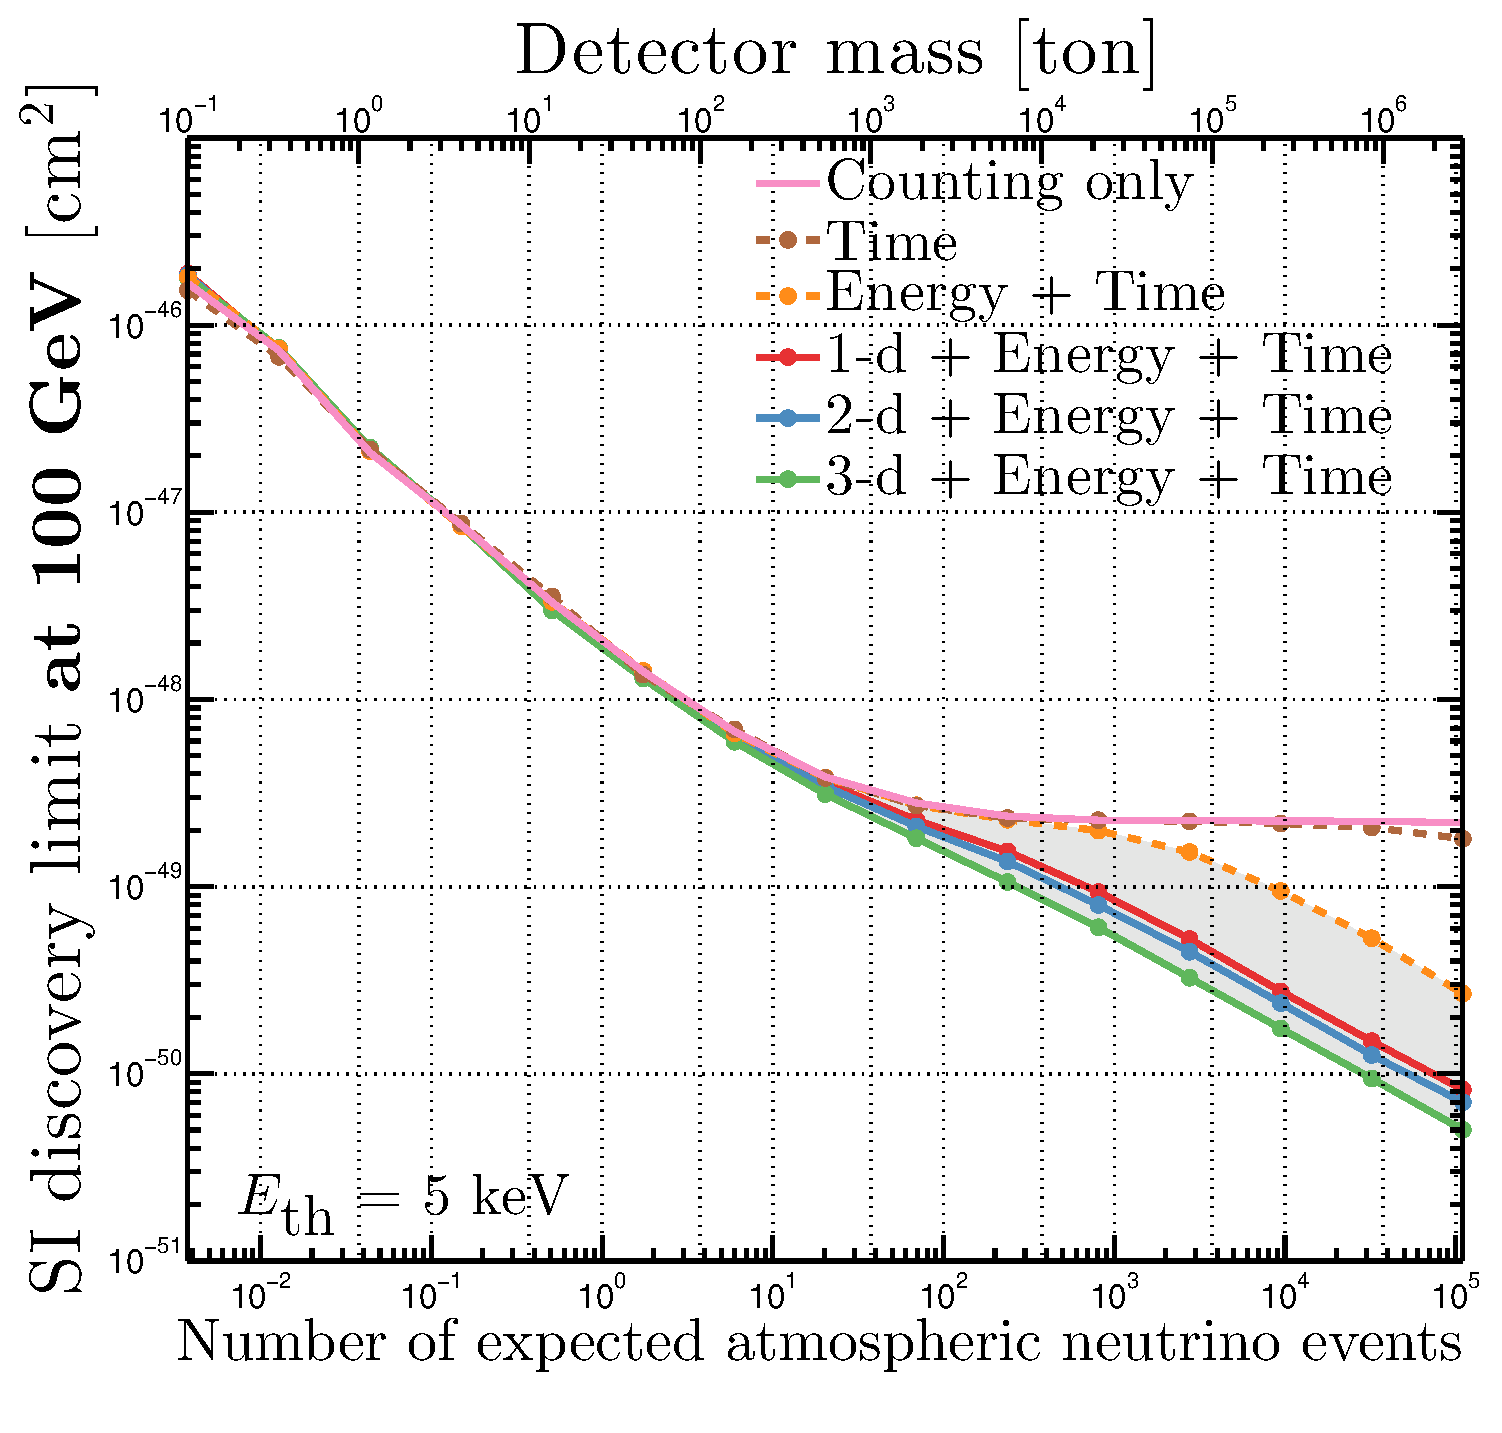
\includegraphics[trim = 0mm 0mm 0mm 0mm, clip,width=0.49\textwidth,angle=0]{Figures/SI_discovery_Xe_100GeV.eps}
\caption[Neutrino floor vs detector mass for different readout strategies]{The dependence of the discovery limit for the SI WIMP-nucleon cross section on the mass of a xenon detector operated for $1 \, {\rm year}$ using  (from top to bottom) 
the number of events only (pink line), time information (brown dashed),  energy \& time (orange dashed), energy \& time  plus 1-d (red), 2-d (blue) and 3-d (green) directionality. 
The left (right) plot is for $m_{\chi} = 6 \, (100) \, {\rm GeV} $ and an energy threshold $E_{\rm th} = 0.1 \, (5) \, {\rm keV}$ and the bottom axis shows the number of ${}^{8}\rm{B}$  (atmospheric) neutrinos expected. 
Note the different scales of the left and right hand plots.} 
\label{fig:detectormass}
\end{center}
\end{figure}

Figure~\ref{fig:detectormass} shows the evolution of the SI discovery limit with increasing detector mass, $M$, using each of the six different readout strategies. We consider two example WIMP masses and detector: a light WIMP \&  low threshold detector ($m_{\chi} = 6$ GeV and $E_{\rm th} = 0.1$ keV) and a 100 GeV WIMP \&  moderate threshold detector ($E_{\rm th} = 5 $ keV). For these two WIMP masses the recoil energy spectra closely matches those of $^8$B and atmospheric neutrinos respectively. It should be emphasised that these thresholds by the standards of directional detectors are very low. However the purpose of this study is to establish whether the neutrino background can be subtracted using directional information, rather than by some specific detector. Indeed, a detector with a threshold above $\sim$5~keV observes no Solar neutrino background at all, so the point is somewhat inconsequential unless we use low thresholds. We note also that there have been methods proposed to look for directional effects in very low energy signals using semiconductors~\cite{Kadribasic:2017obi}.

The evolution of the discovery limit develops as a function of $M$ (or equivalently neutrino event number) in a number of phases as we have already described in Sec.~\ref{sec:nufloor_nufluxunc}. Notably, when the expected number of neutrino events reaches $10-10^{2}$ the counting only, time only, as well as the energy \& time limits all plateau\footnote{Interestingly we see that timing information here seems to be more useful for discriminating Solar neutrinos from light WIMPs than for discriminating atmospheric neutrinos from heavier WIMPs. We can attribute this to the fact that the WIMP and Solar neutrino rates are both annually modulated, and also the amplitude of the annual modulation is larger for lighter WIMPs (cf. Fig.~\ref{fig:AnnualDailyModulation}).}. The limits with directional readout however continue to decrease as the incorporation of directional information allows the distributions of WIMP and neutrino induced recoils to be distinguished. For the 100 GeV WIMP case, the limits from 2-d and 3-d readout are a factor of $\sim 1.2$ and $1.6$ better than those from 1-d readout whereas for the 6 GeV WIMP case they are factors of $\sim 1.2$ and $3$ times better. The discovery limit with directionality continues to decrease as $\propto 1/M$ for the 6 GeV WIMP as the directional and time-dependent distributions of the WIMP and Solar neutrino induced recoils have such a small overlap that the background has very little effect on the discovery capabilities of the experiment. However for the 100 GeV WIMP the dominant background from atmospheric neutrinos significantly overlaps with the WIMP distribution so, although the experiment is able to distinguish the WIMP signal, the sensitivity is still compromised by the background. In this case the discovery limit, beyond the saturation regime, evolves according to a standard Poisson background subtraction mode $\propto 1/\sqrt{M}$.

\begin{figure}
\begin{center}
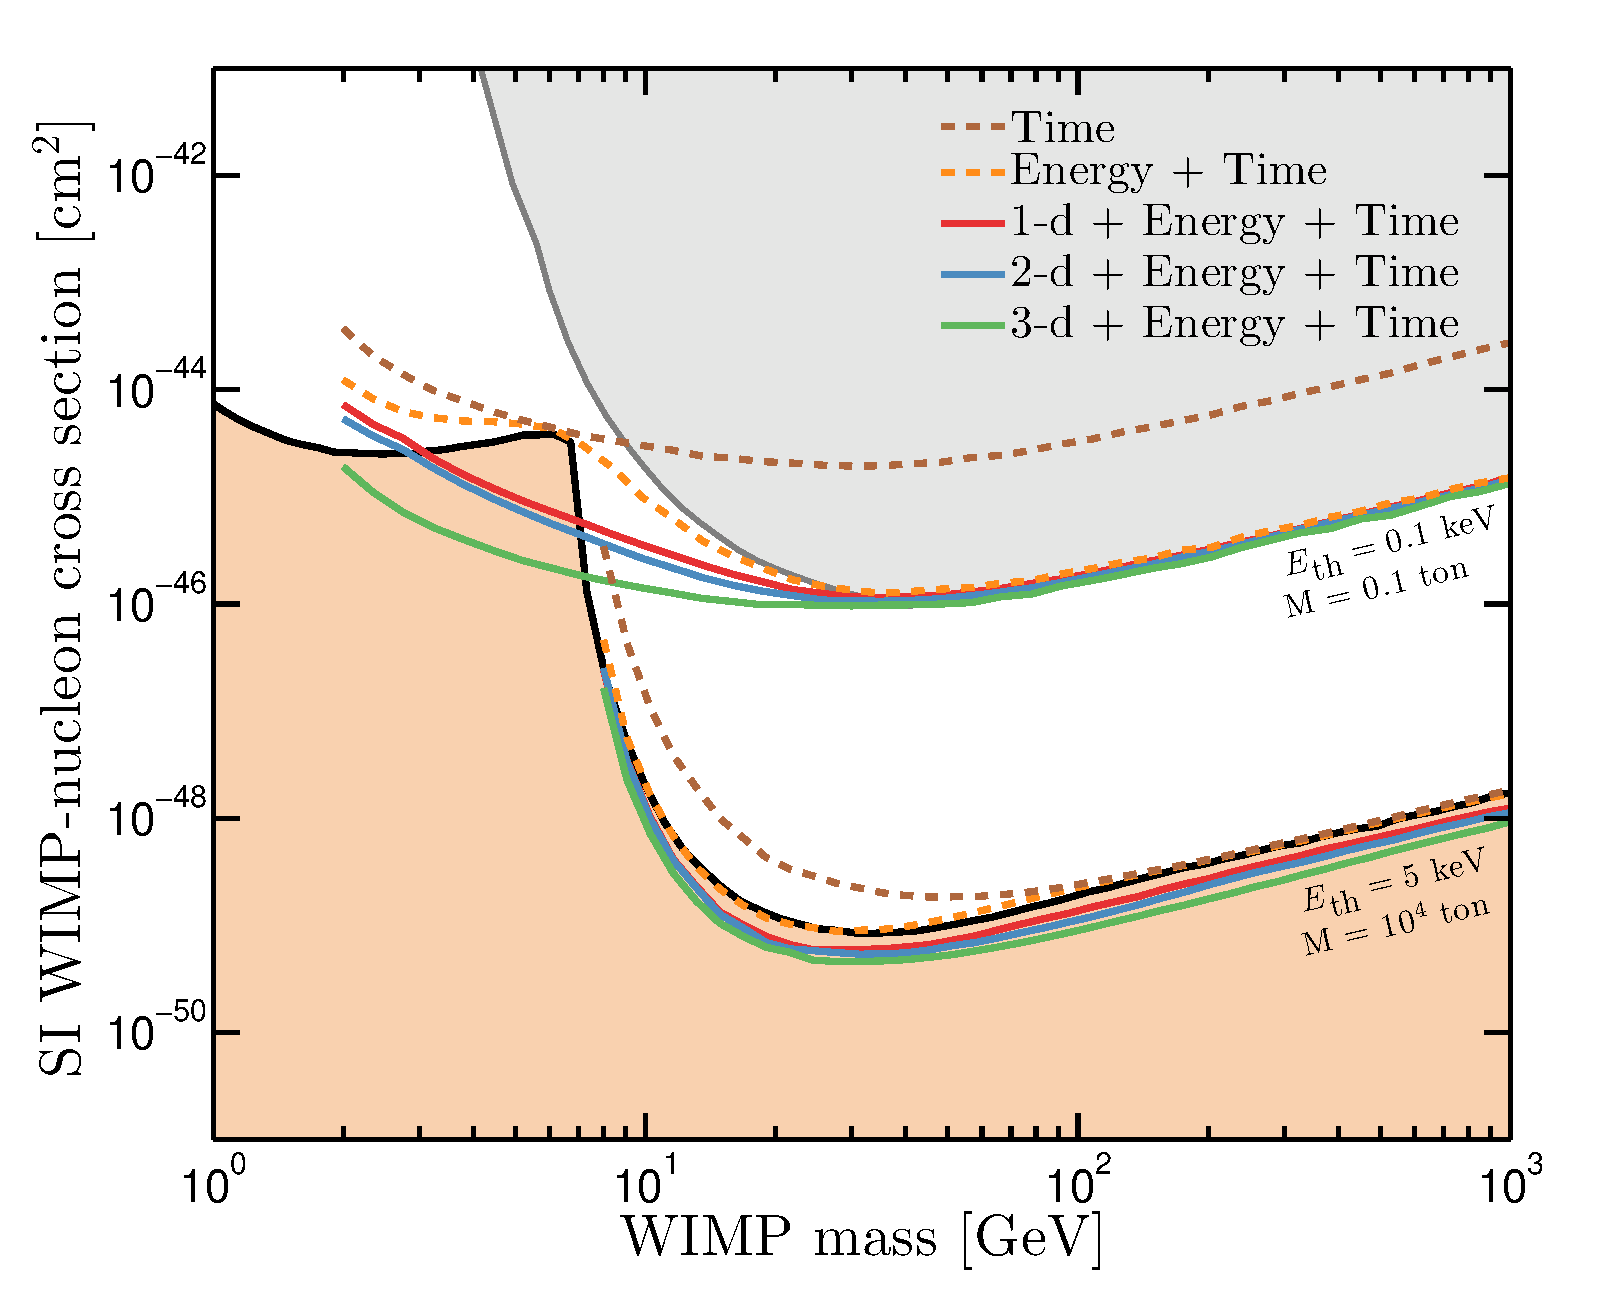
\includegraphics[width=0.8\textwidth,angle=0]{Figures/ReadOut_Comparison_floors.eps}
\caption[Comparison of discovery limits with different readout strategies]{%The discovery limit for the spin independent WIMP-nucleon cross section, $\sigma_{\rm p}^{\rm SI}$, as a function of WIMP mass for a ${\rm Xe}$ detector operated for $1 \, {\rm year}$ 
The discovery limit
%, as in Fig.~\ref{fig:detectormass},
as a function of WIMP mass using (from top to bottom): time information (brown dashed),  energy \& time (orange dashed), 1-d (red), 2-d (blue) and 3-d (green) directionality. 
The upper (lower) set of lines are for the detector set-up with target mass $M=0.1 \, (10^4)$ tons and threshold $E_{\rm th} = 0.1 \, (5) \, {\rm keV}$. 
The orange region shows the neutrino floor from Ref.~\cite{Ruppin:2014bra}. The grey region covers parameters already excluded by experiments.} 
\label{fig:readoutfloors}
\end{center}
\end{figure} 

Having studied the evolution of the discovery limit as a function of detector mass for two specific WIMP masses, we now consider two fixed example detector set-ups: a low mass \& low threshold detector ($M=0.1$ ton and $E_{\rm th} = 0.1 \, {\rm keV}$ respectively) and a high mass \& moderate threshold detector ($10^4$ ton and 5 keV). These detector masses and thresholds are chosen so that a non-directional detector with the same mass and threshold would be in the saturation regime that results in the neutrino floor, as seen in Fig.~\ref{fig:detectormass}. Figure~\ref{fig:readoutfloors} shows the discovery limit as a function of WIMP mass for these two detector set-ups and each readout strategy. Also shown as the orange shaded region is the well known neutrino floor from Ref.~\cite{Ruppin:2014bra} which is the concatenation of two separate limits roughly matching our two detector setups\footnote{For light WIMPs ($m_{\chi} <10$ GeV) the limit comes from a 3 eV threshold detector with an exposure of 0.19 ton years, while for heavier WIMPs ($m_{\chi} >10$ GeV) a detector with a 4 keV threshold and an exposure of $9.3 \times 10^3$ ton years was used.}.

For the low threshold detector, the directional discovery limits clearly cut through the light WIMP neutrino floor and for the 3-d readout there is almost no reduction in sensitivity due to the neutrino background. The 1-d and 2-d readouts do suffer a small reduction in sensitivity, but evidently the distributions are different enough that it is still possible to probe cross sections below the limit set by non-directional experiments. For the high threshold detector the improvement in the discovery limits, with respect to the high-mass neutrino floor, from directionality is smaller. However it does still help discriminate the isotropic atmospheric neutrino background from WIMP induced recoils, in particular for WIMP masses around $100 \, {\rm GeV}$ where the energy spectra from WIMPs and atmospheric neutrinos are most similar.

In summary, we find that directionality is a powerful tool for disentangling neutrino backgrounds from a WIMP signal. The gain from directionality is particularly impressive for low mass WIMPs thanks to the large separation between the Solar neutrino and WIMP incoming directions (cf. Sec.~\ref{sec:nufloor_signals}). We also find that this result still holds even if only the 2-d or 1-d projection of the recoil tracks can be measured.


\subsection{Non-ideal detectors}\label{sec:nufloor_nonideal}
\label{sec:nufloor_sense}
\begin{figure}
\begin{center}
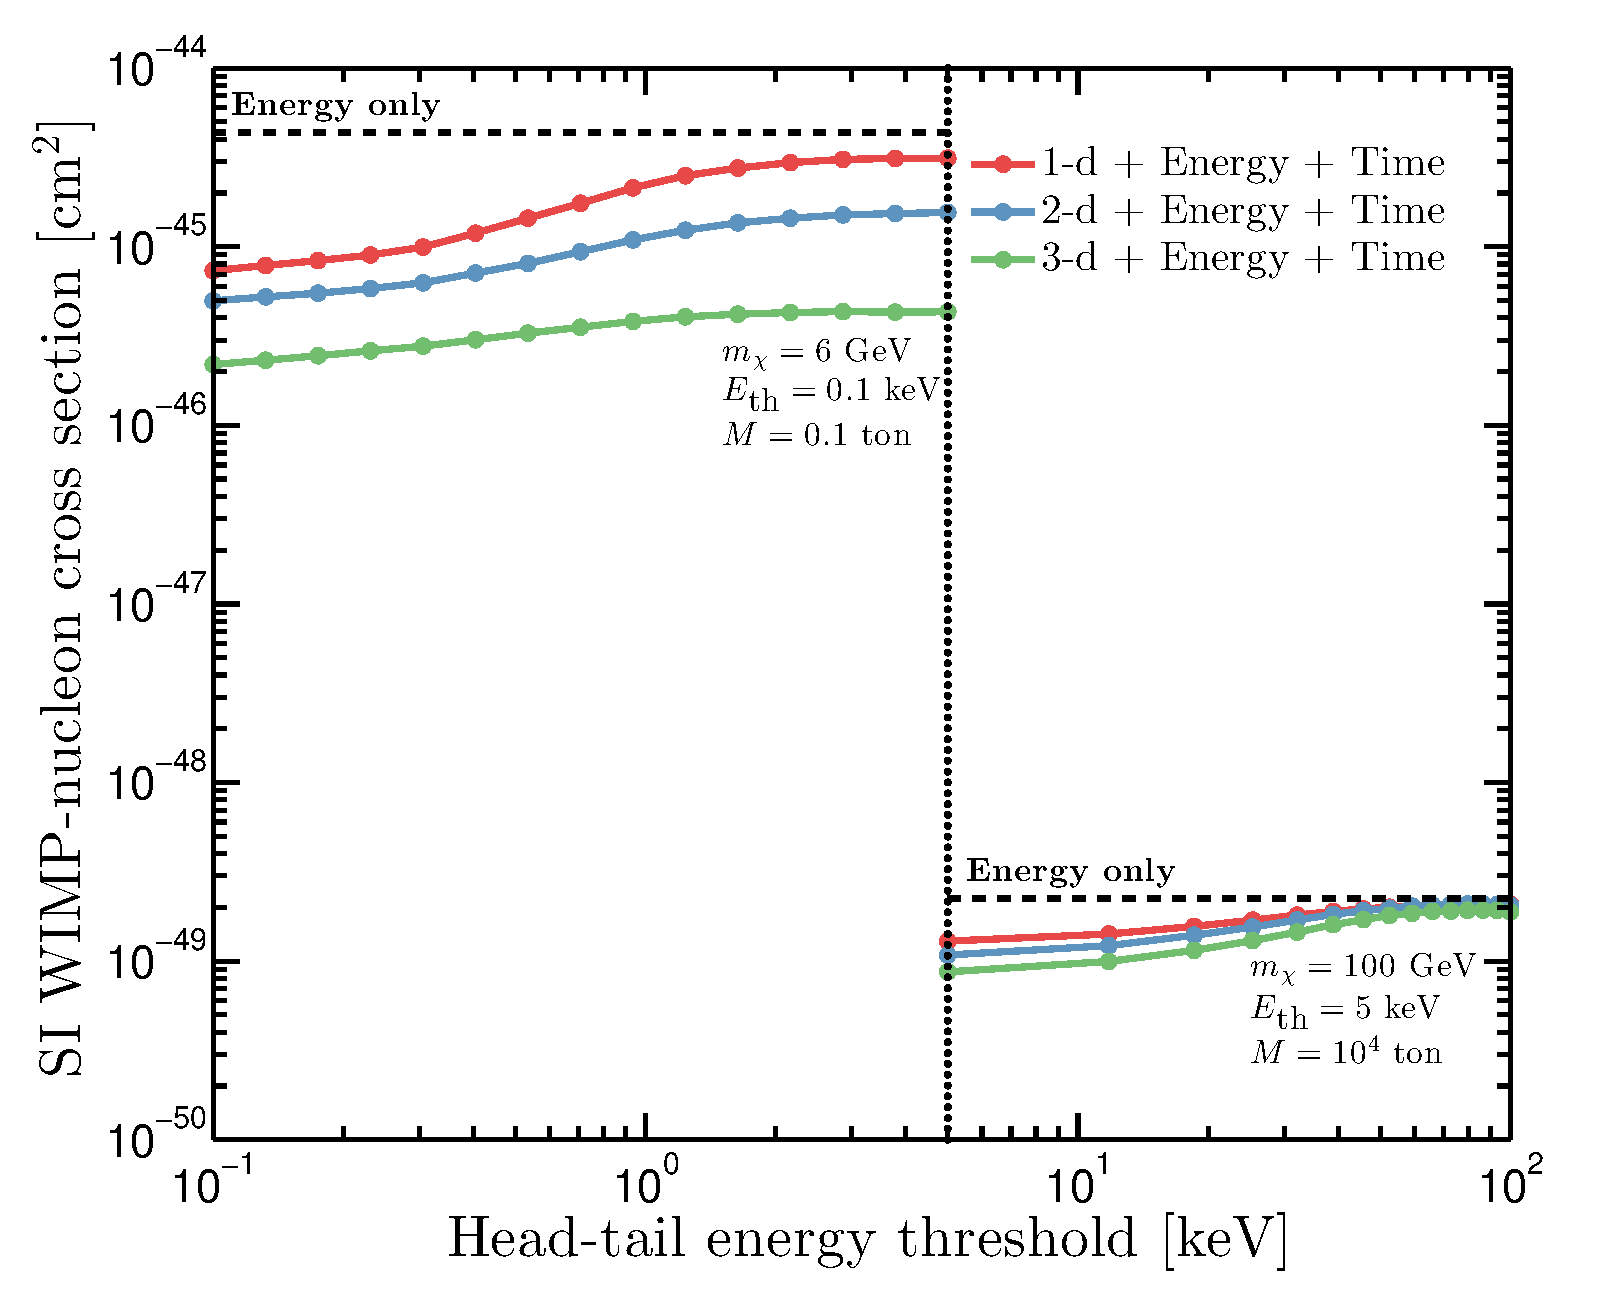
\includegraphics[width=0.8\textwidth,angle=0]{Figures/HeadTail_combined.eps}
\caption[Neutrino floor as a function of head-tail discrimination threshold]{
The discovery limit as a function of the energy threshold for head-tail discrimination for 1-d (red), 2-d (blue) and 3-d (green) directional readout (with energy and time information in all three cases). The dashed orange line shows the discovery limit with energy information only.
The left (right) set of lines correspond to the discovery limits at 6 (100) GeV made by the detector set-up with target mass $M=0.1 \, (10^4)$ tons and threshold $E_{\rm th} = 0.1 \, (5) \, {\rm keV}$. }
%a detector with a target mass $M=0.1 \, (10^4)$ ton and an energy threshold $E_{\rm th} = 0.1 \, (5) \, {\rm keV}$.} 
\label{fig:headtail}
\end{center}
\end{figure} 

\begin{figure}
\begin{center}
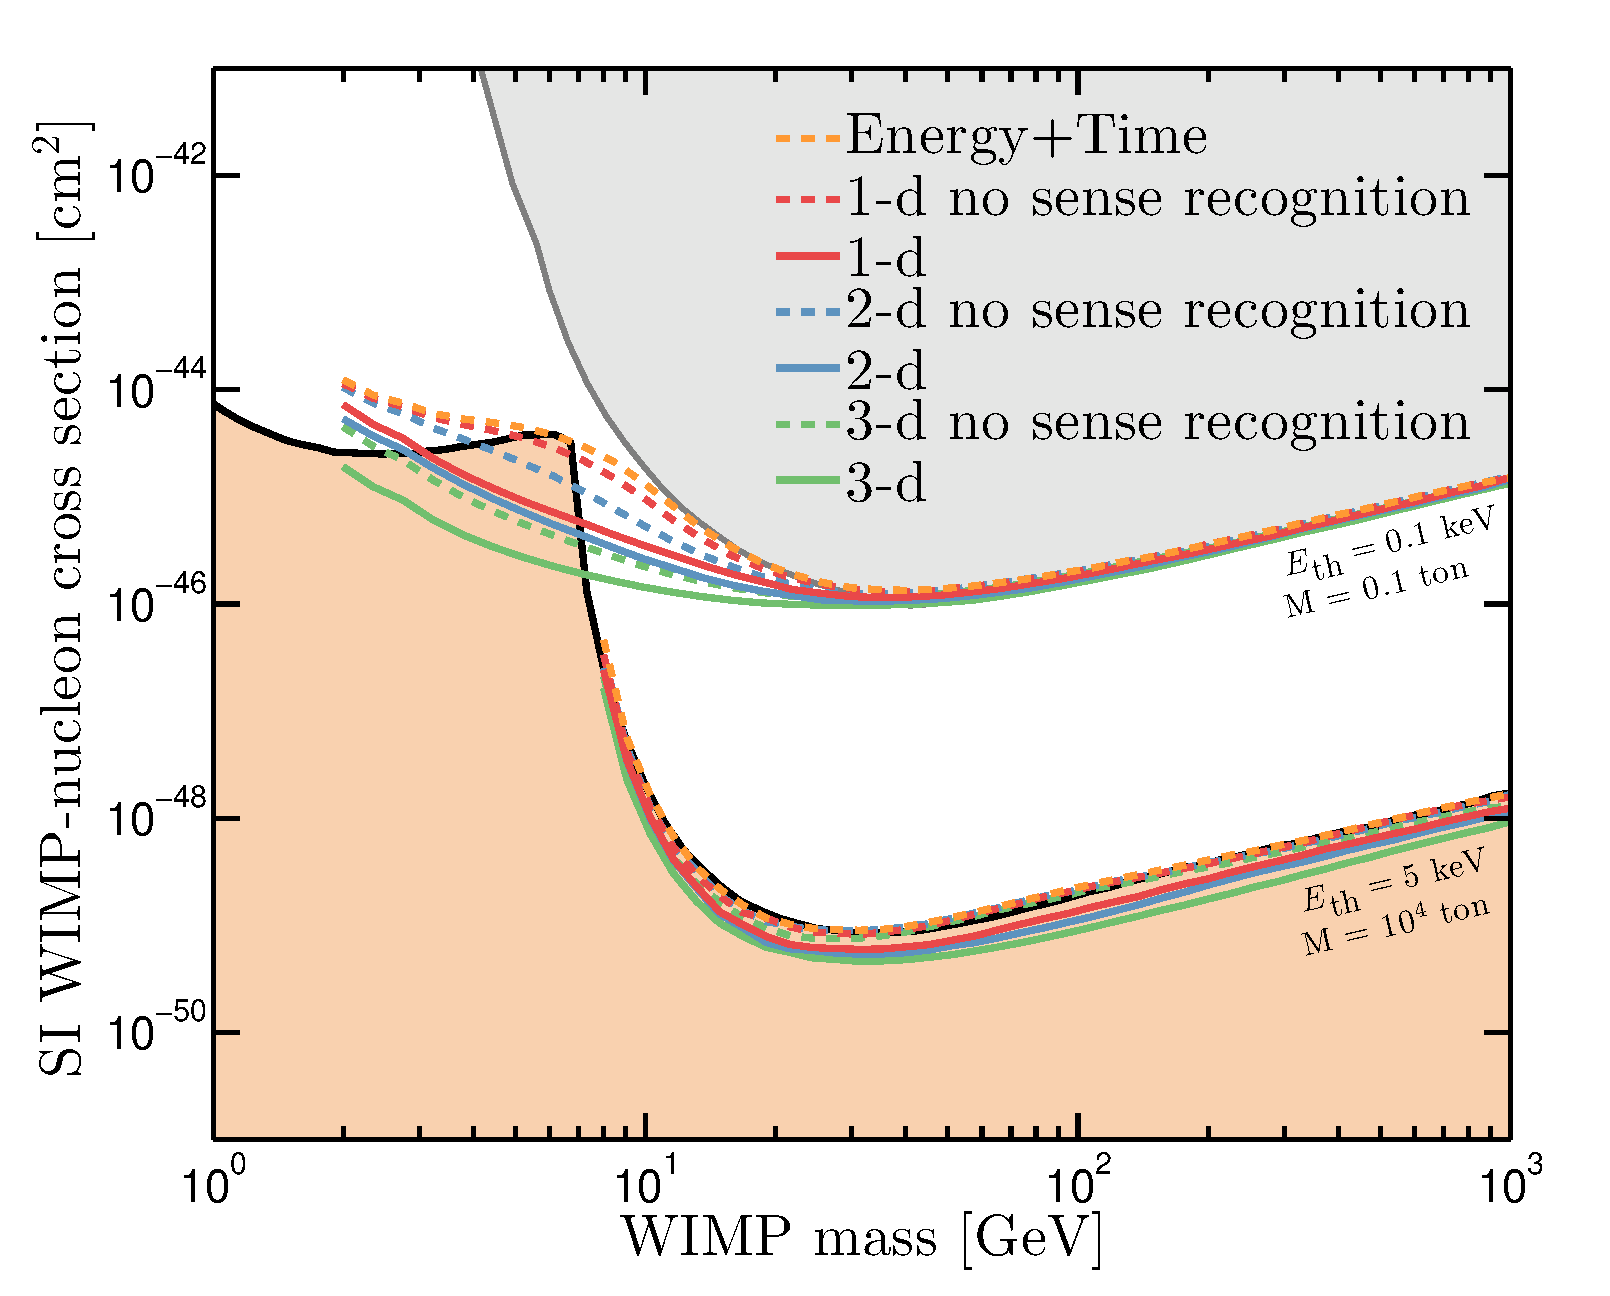
\includegraphics[width=0.8\textwidth,angle=0]{Figures/HeadTail_floors.eps}
\caption[Neutrino floor for directional detectors with no sense recognition]{The discovery limit as a function of WIMP mass for detectors with full sense recognition (solid lines) and no sense recognition (dashed) and 1-d (red), 2-d (blue) and 3-d (green) directional readout. The upper (lower) set of lines are for the detector set-up with target mass $M=0.1 \, (10^4)$ tons and threshold $E_{\rm th} = 0.1 \, (5) \, {\rm keV}$. The dashed orange lines show our discovery limit with energy information only and
the orange region shows the neutrino floor from Ref.~\cite{Ruppin:2014bra}. The grey region covers parameters already excluded by experiments.}
\label{fig:headtailfloors}
\end{center}
\end{figure} 

\begin{figure}
\begin{center}
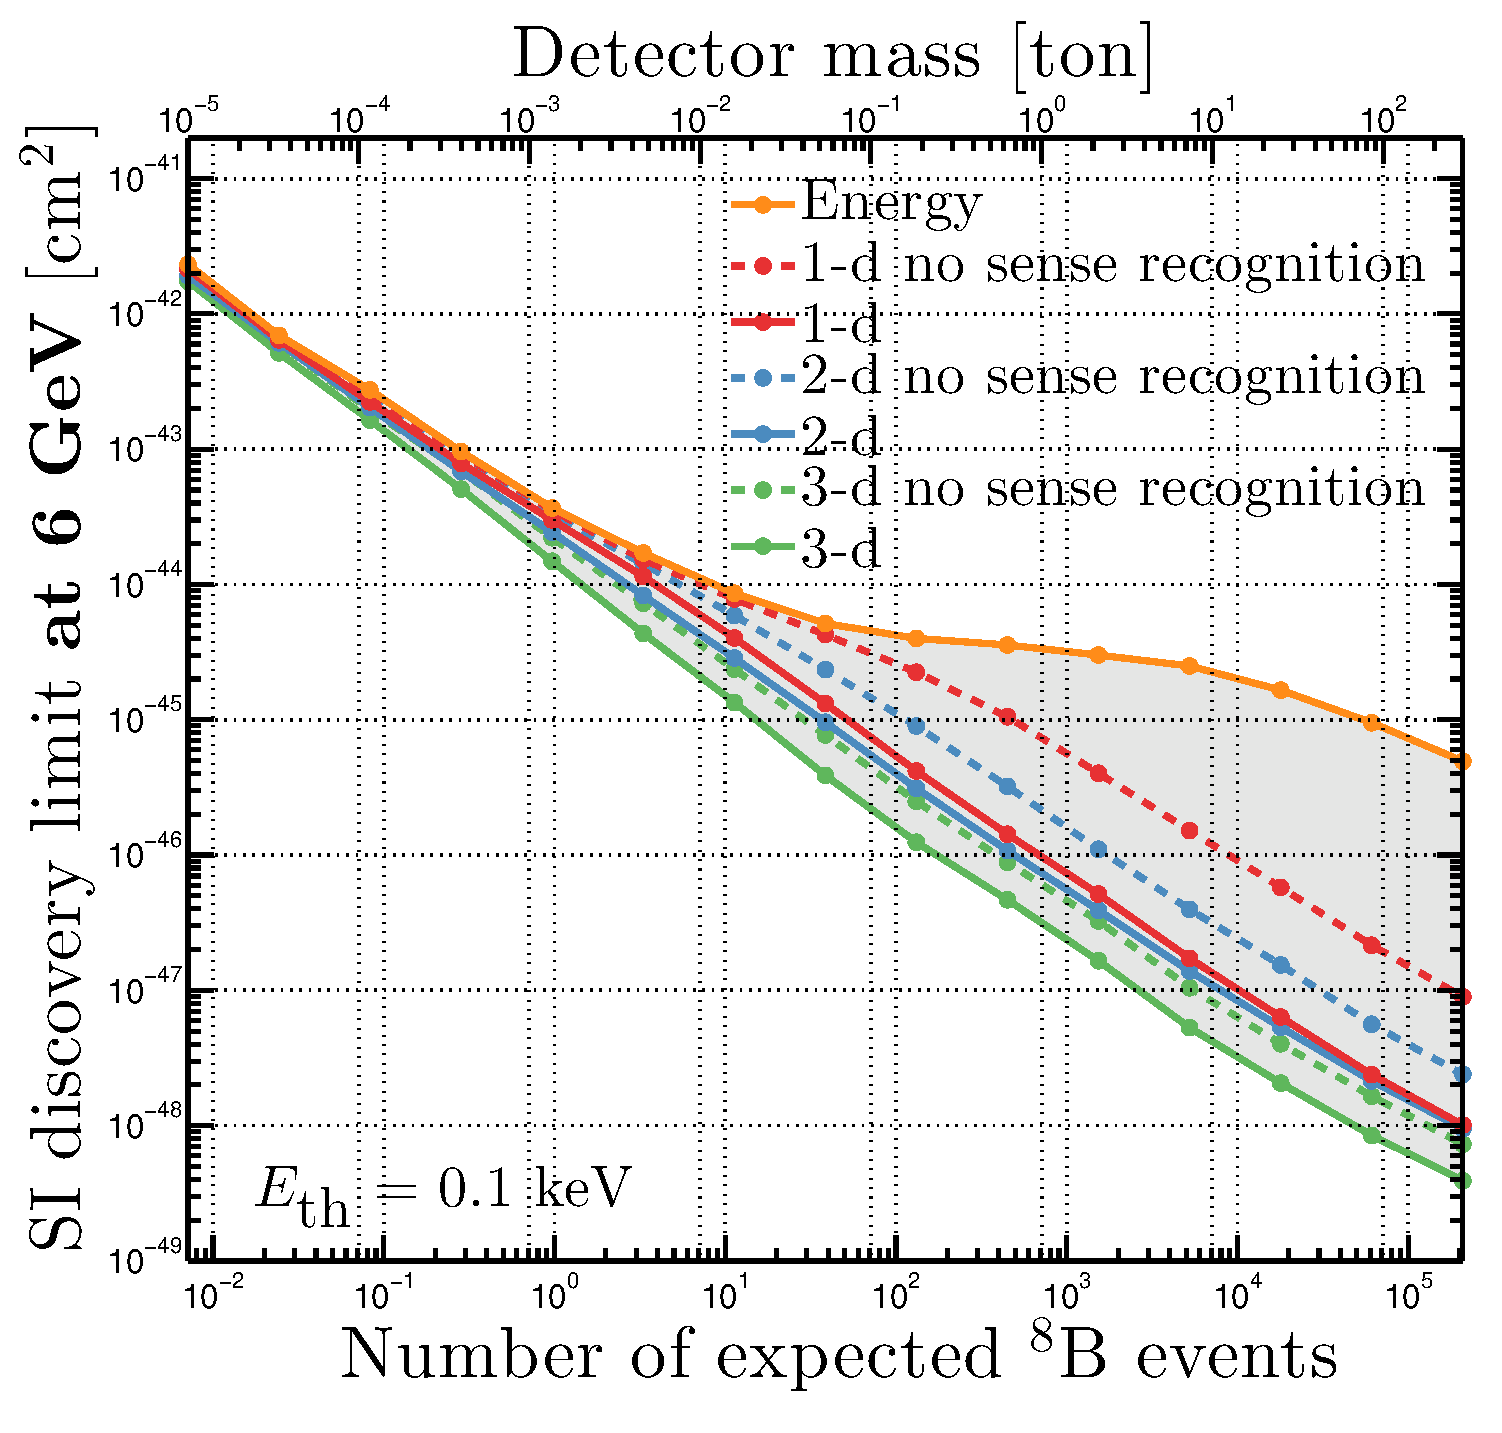
\includegraphics[trim = 0mm 0mm 0mm 0mm,clip,width=0.49\textwidth,angle=0]{Figures/HeadTail_sig_vs_Exposure_6GeV.eps}
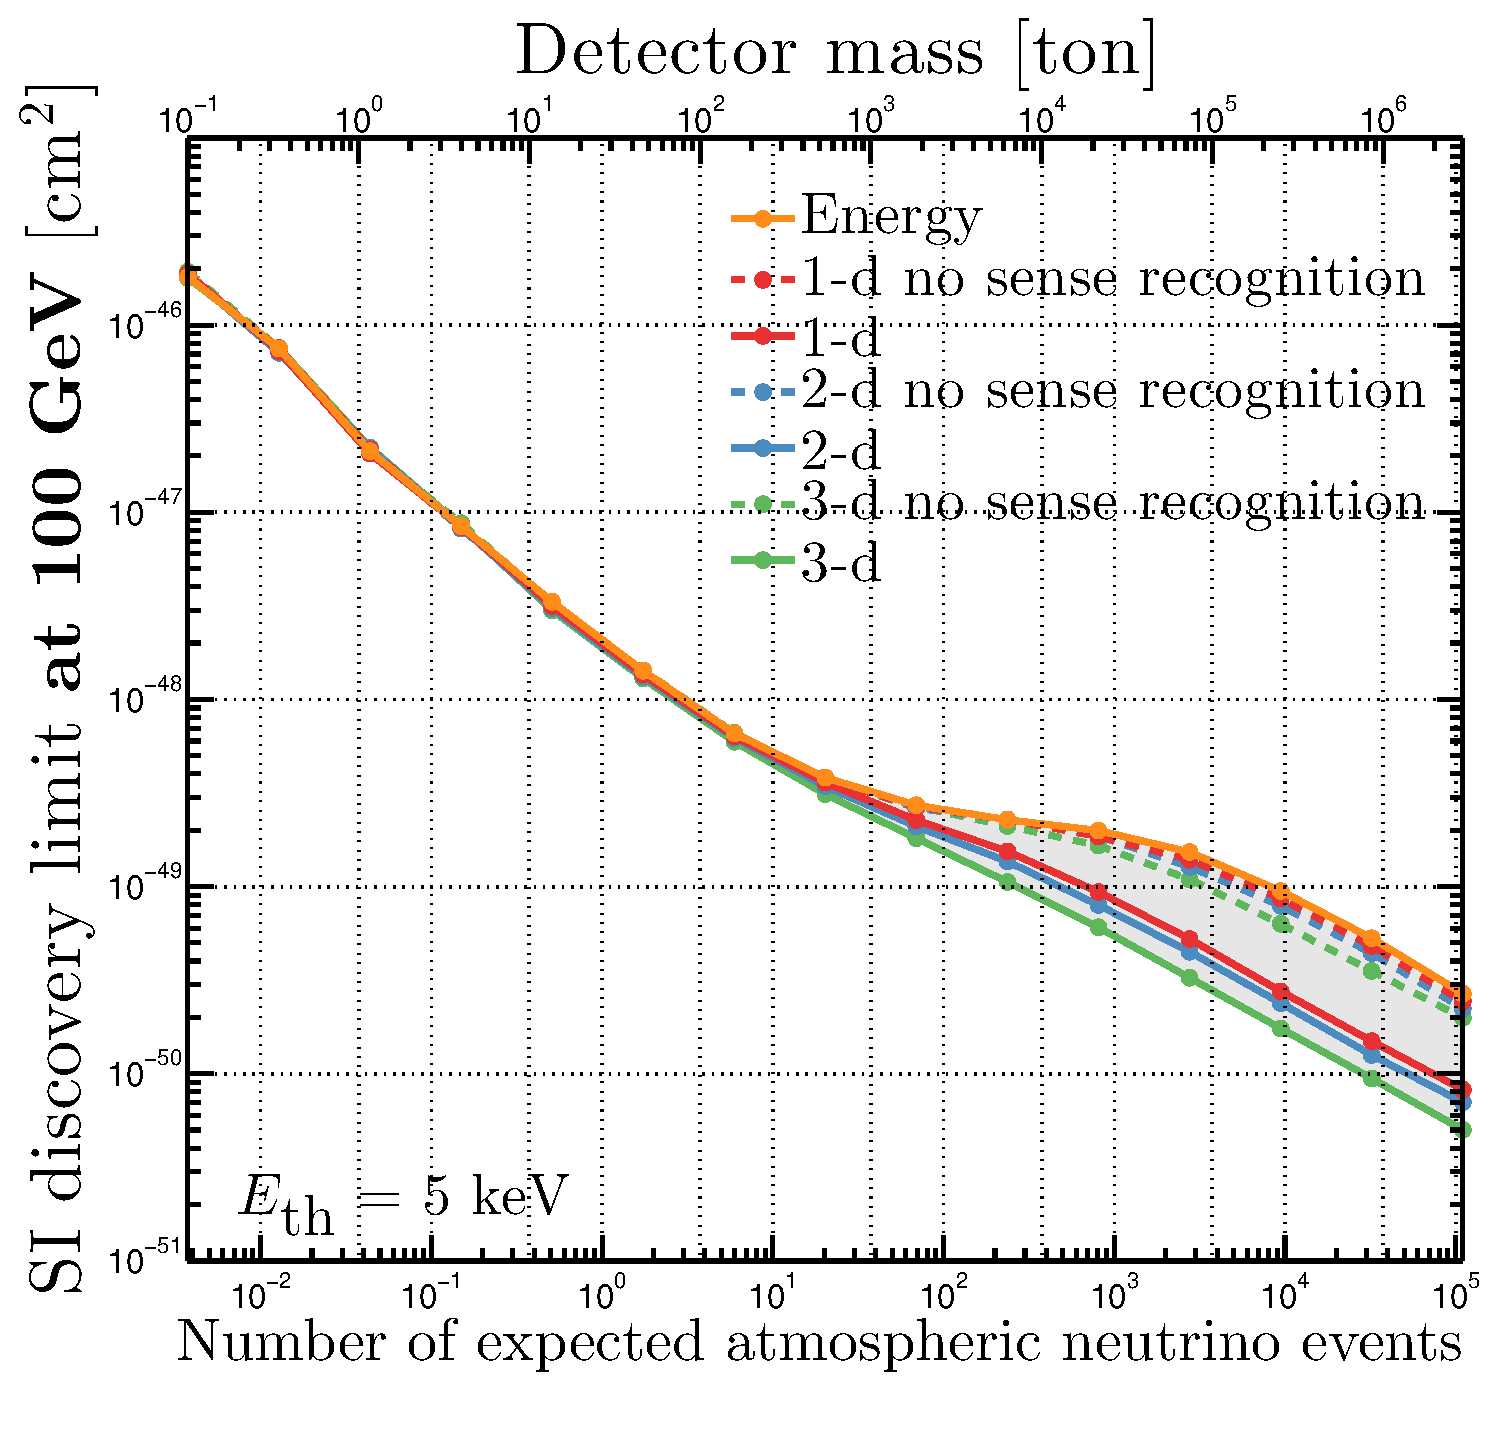
\includegraphics[trim = 0mm 0mm 0mm 0mm,clip,width=0.49\textwidth,angle=0]{Figures/HeadTail_sig_vs_Exposure_100GeV.eps}
\caption[Neutrino floor vs detector mass with no sense recognition]{The dependence of the discovery limit for the SI WIMP-nucleon cross section on detector mass for detectors with (solid lines) and without (dashed lines) sense recognition for each of the three directional readout strategies 3-d (green), 2-d (blue) and 1-d (red). The discovery limit for energy + time only readout is shown with the orange lines. The left (right) panel is for 
$m_{\chi} = 6 \, (100) \, {\rm GeV} $ and detector set-up with threshold $E_{\rm th} = 0.1 \, (5) \, {\rm keV}$. \label{fig:headtailmass}}
%The dependence is shown for the same two WIMP mass cases as in Fig.~\ref{fig:detectormass}, left: 6 GeV (with a 0.1 keV threshold), and right: 100 GeV (with a 5 keV threshold).} 
\end{center}
\end{figure}

We now move beyond the ideal situation and consider two limitations particular to directional experiments: head-tail (sense) recognition and angular resolution. 

{\bf Head-tail recognition}, as we have already discussed, is one of the most important considerations for the discovery reach of directional experiments. Head-tail effects based on charge deposition or track geometry are naturally more apparent at larger recoil energies. Figure~\ref{fig:headtail} shows how the discovery limit depends on the {\it threshold} for head-tail discrimination.
For simplicity, we assume that below the head-tail energy threshold there can be no sense discrimination.
For the light WIMP and the low mass and threshold detector, the discovery limits are weakened as the head-tail energy threshold is increased from $0.1 \, {\rm keV}$ to $\sim 1-2 \, {\rm keV}$ before flattening off to a factor between $\sim 1.5$ (for 1-d)  and $\sim 10$ (for 3-d) below the energy only limit. For lower dimensional readout the decrease in sensitivity is larger and the plateau in the limit is reached for a larger head-tail energy threshold. Qualitatively similar behaviour occurs for the $100 \, {\rm GeV} $ WIMP and the higher mass and threshold detector. In this case the discovery limits flatten off to values $1.1 - 1.2$ below the
energy only limit at a head-tail energy threshold of $60 \, {\rm keV}$. 

In Figure~\ref{fig:headtailfloors} we show the discovery limits with and without sense recognition, as a function of WIMP mass. The factor by which the discovery limit changes without sense recognition is largest for light, $m_{\chi} < {\cal O}(20 \, {\rm GeV})$, WIMPs and a low threshold. The discovery limit achieved by a 3-d readout is still considerably lower than the non-directional limit however 1-d and 2-d readouts do suffer without sense recognition and are only marginally better than the non-directional limits, especially at high WIMP masses.

In Figure~\ref{fig:headtailmass} we show (in similar fashion to Fig.~\ref{fig:detectormass}) the evolution of the discovery limit now as a function of detector mass for $m_{\chi} = 6$ and $100 \, {\rm GeV} $ with and without sense.
As in Fig.~\ref{fig:headtailfloors}, we see that the lack of sense recognition is most damaging in the 100 GeV WIMP case. This is particularly true for the 1-d and 2-d readouts, with no sense recognition there is only a factor of 1.1 and 1.2 improvement over a detector with no directional information at all and the evolution of the discovery limit suffers from a similar (but less severe) saturation effect due to the overlapping recoil distributions. In the 6 GeV WIMP case the discovery limits with no sense recognition continue to decrease past the saturation regime suffered by the non-directional limit. However there is still a reduction in sensitivity by factors of 1.9, 2.8 and 8.9 for 3-d, 2-d and 1-d readouts respectively compared to the limits with sense recognition. Interestingly, the discovery limit for 3-d readout with no sense recognition is slightly better than 1-d and 2-d readouts with sense recognition. 

Our main conclusion regarding sense recognition is that for discriminating between Solar neutrinos and low mass WIMPs, having 3-d readout with no method of determining sense is marginally preferable to 1-d or 2-d readout with sense determination. 
This is because the recoil distributions from low mass WIMPs and Solar neutrinos are both anisotropic and have sufficient 3-d angular separation that they are still distinguishable even without recoil sense information. For the higher mass WIMPs this is not the case, and 
without sense recognition the advantage of directionality is almost entirely lost, even in 3-d.


{\bf Angular resolution} is limited by the inaccuracy in the estimation of the ``true'' recoil direction. This is an inherent difficulty faced by all directional detectors. Finite angular resolution will smear out the WIMP and Solar neutrino distributions in Fig.~\ref{fig:Moll}, making it more difficult to discriminate between the two. Since the minimum separation between the peak WIMP and neutrino directions is $\sim60^\circ$, an angular resolution better than this will likely be required to differentiate between the WIMP and Solar neutrino distributions.

Finite angular resolution results in a recoil in the direction $\hat{\textbf{q}}'(\Omega'_r)$ reconstructed in the direction $\hat{\textbf{q}}(\Omega_r)$ with a probability distribution that takes the form of a Gaussian smoothing kernel on a sphere~\cite{Copi:2005ya,Billard:2011zj}
\be
K(\Omega_r,\Omega_r') = \frac{1}{ (2\pi)^{3/2} \sigma_\gamma \rm{erf}(\sqrt{2}\sigma_\gamma)   } \exp{\left( - \frac{\gamma^2}{2\sigma_\gamma^2} \right)} \,,
\ee
where $\gamma$ is the angle between the original and reconstructed directions,
\be
\cos{\gamma} = \hat{\textbf{q}}'\cdot\hat{\textbf{q}} = \sin{\theta}\sin{\theta'}\cos{(\phi-\phi')} + \cos{\theta}\cos{\theta'}\,,
\ee
in the coordinates defined in Eq.~(\ref{eq:angles}). The measured directional recoil rate is then the convolution of the smoothing kernel with the original directional recoil rate
\be
\frac{{\rm d}^2 R}{\rm{d} \Omega_r \rm{d}E_r} = \int_{\Omega'_r} \frac{{\rm d}^2 R}{\rm{d} \Omega'_r \rm{d}E_r} K(\Omega_r,\Omega'_r) \, {\rm d} \Omega'_r \,.
\ee
\begin{figure}
\begin{center}
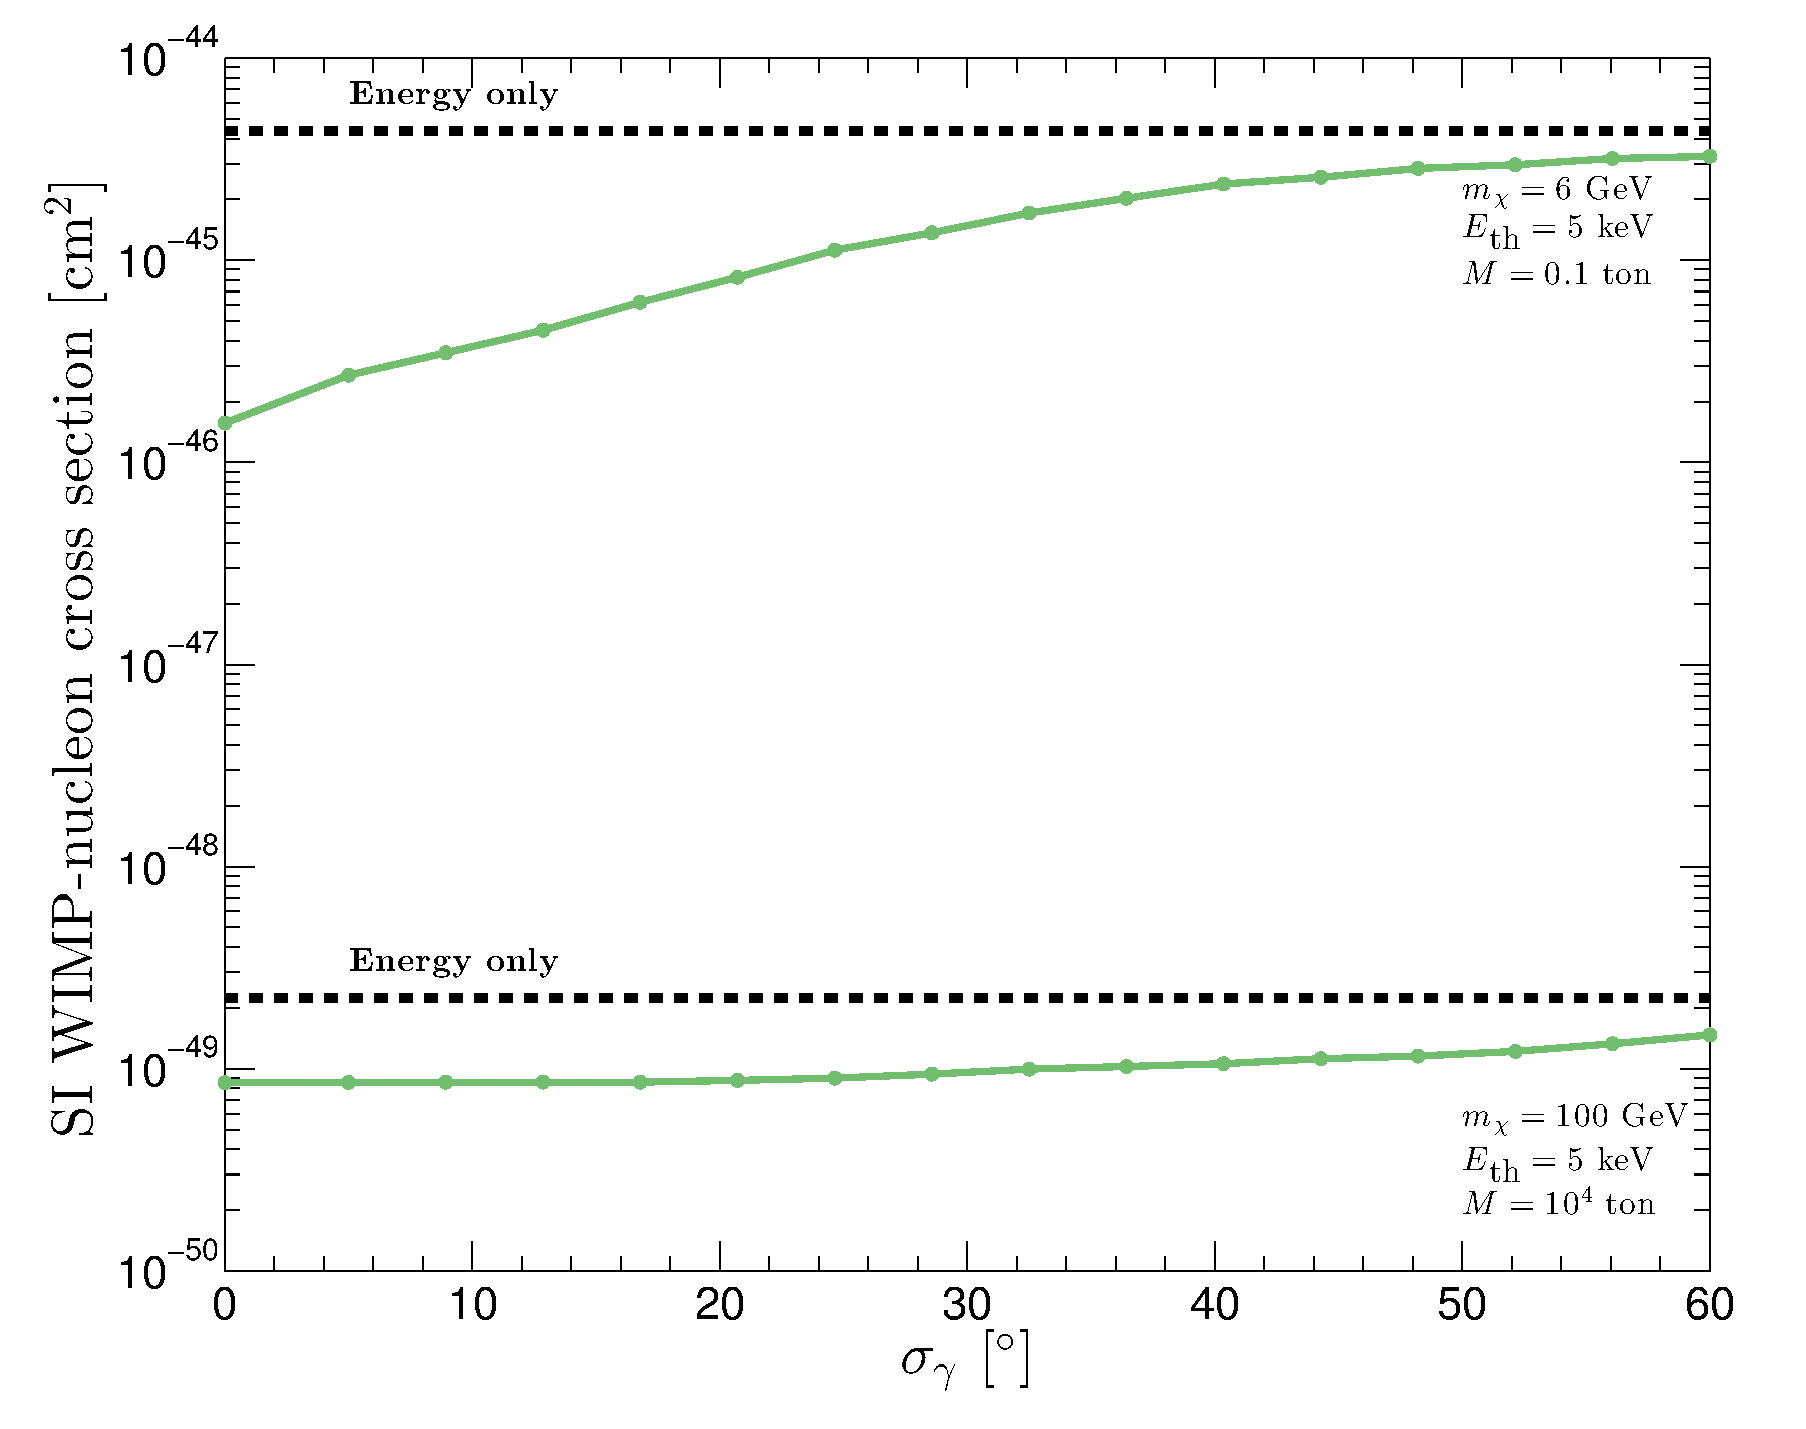
\includegraphics[width=0.8\textwidth,angle=0]{Figures/AngRes_100GeV_6GeV-eps-converted-to.pdf}
\caption[The discovery limit as a function of angular resolution]{ The discovery limit as a function of angular resolution, $\sigma_\gamma$ for a detector with 3-d readout.  
The upper (lower) set of lines are for $m_{\chi} = 6 \, (100) \, {\rm GeV}$. The upper (lower) line is for the detector set-up with threshold $E_{\rm th} = 0.1 \, (5) \, {\rm keV}$.   
The dashed lines show the discovery limit using energy information only. }
\label{fig:angressingle}
\end{center}
\end{figure} 

\begin{figure}
\begin{center}
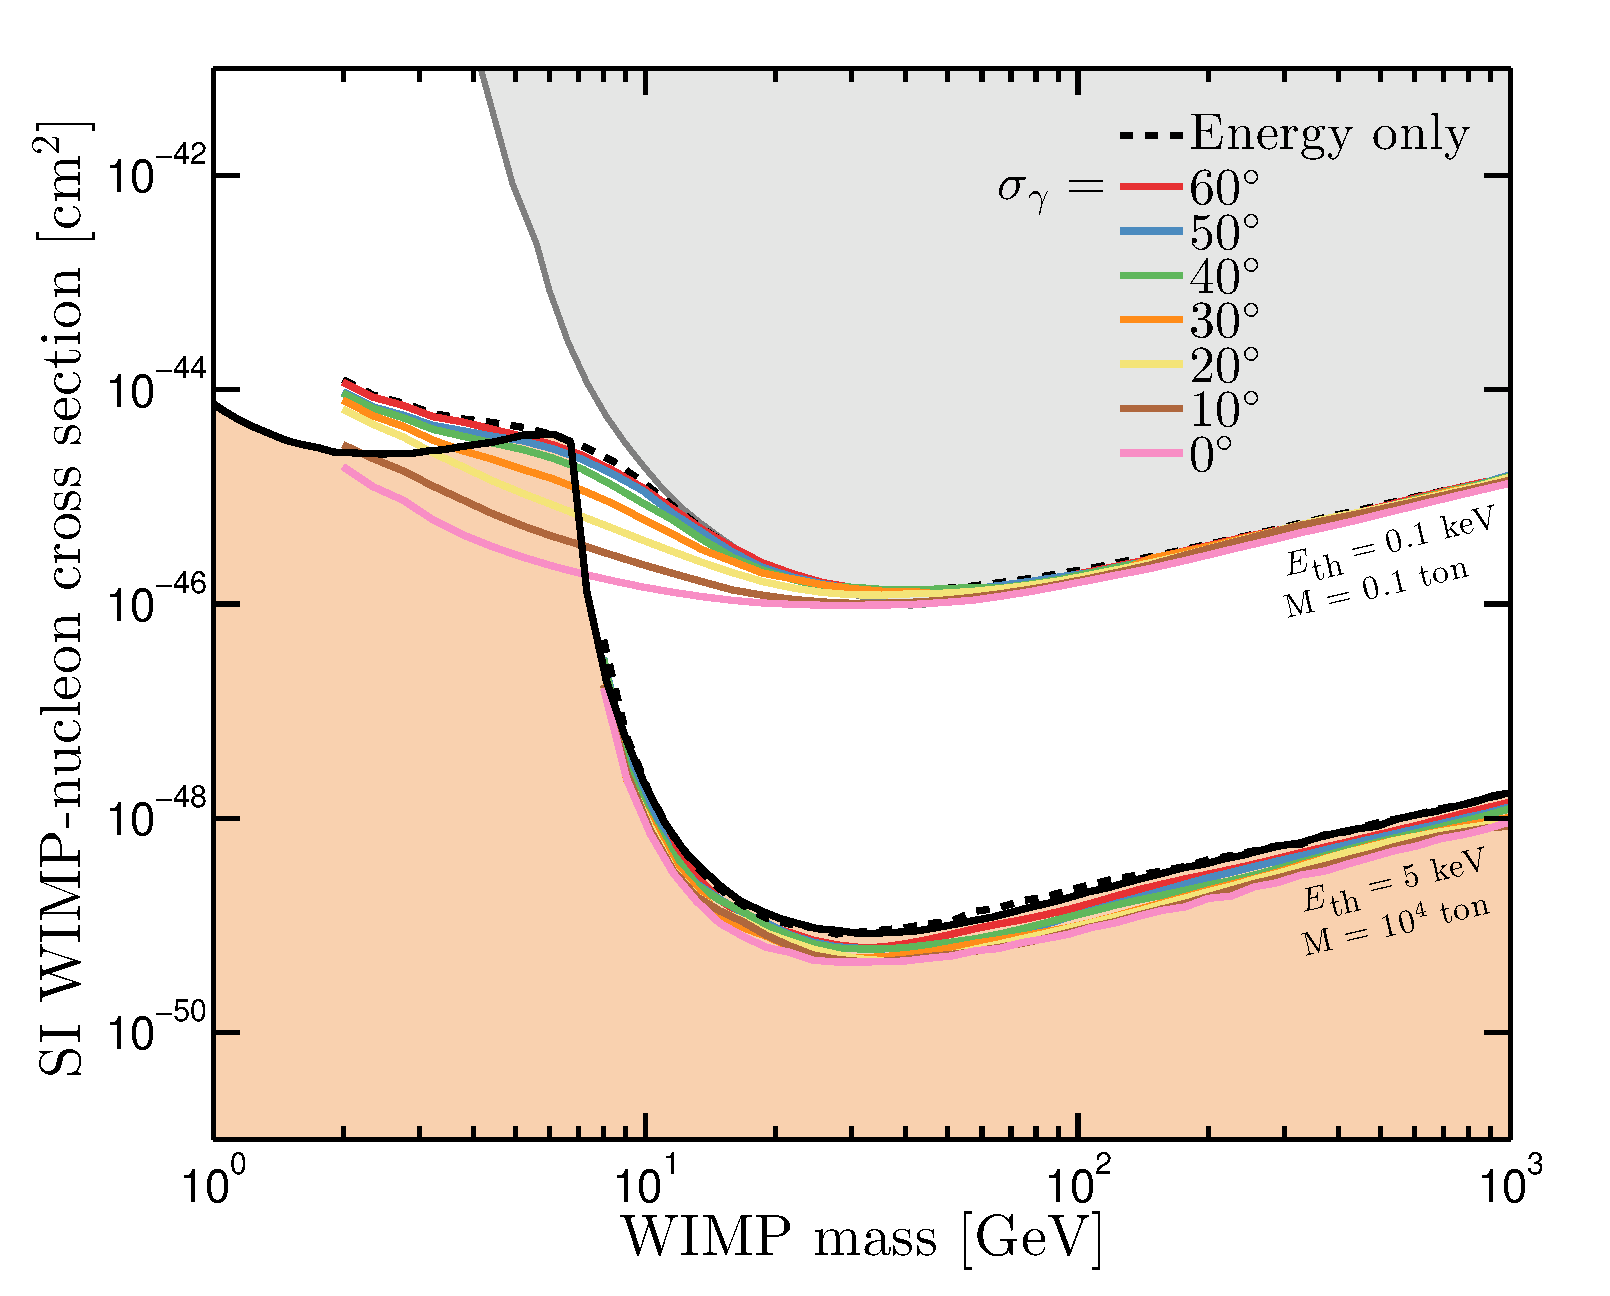
\includegraphics[width=0.8\textwidth,angle=0]{Figures/AngRes_floors.eps}
\caption[Neutrino floor as a function of angular resolution]{The discovery limit, as in Fig.~\ref{fig:readoutfloors}, as a function of WIMP mass with angular resolution, $\sigma_\gamma$, varying between $0^{\circ}$ and $60^{\circ}$ for a detector with 3-d readout. 
The upper (lower) set of lines are for the detector set-up with target mass $M=0.1 \, (10^4)$ tons and threshold $E_{\rm th} = 0.1 \, (5) \, {\rm keV}$.  
The dashed black lines show our discovery limit with energy information only and
the orange shaded region shows the neutrino floor from Ref.~\cite{Ruppin:2014bra}. The grey region covers parameters already excluded by experiments.
} 
\label{fig:angresfloors}
\end{center}
\end{figure} 

The discovery limit as a function of angular resolution, $\sigma_\gamma$, is shown in Fig.~\ref{fig:angressingle} for
$m_{\chi} = 6$ and $100 \, {\rm GeV} $ for our two example detector set-ups with 3-d readout. As expected,  finite resolution makes it harder to discriminate a $6 \, {\rm GeV}$ WIMP from Solar neutrinos. The discovery limit is an order of magnitude weaker for $\sigma_{\gamma} = 30^{\circ}$ than for perfect angular resolution, and for $\sigma_{\gamma} > 50^{\circ}$ the limit is only marginally better than that obtained using energy information only. For the heavier WIMP and the more massive detector, the discovery limit only has a slight change with increasing $\sigma_\gamma$. This is because the finite angular resolution affects only the WIMP signal and not the atmospheric neutrino background. However in this case the improvement afforded by directionality, even in the ideal case, is smaller.

Figure~\ref{fig:angresfloors} shows the discovery limits for the two detector set-ups as a function of WIMP mass and angular resolution. Finite angular resolution significantly limits the ability of a low threshold directional detector to discriminate light, $m_{\chi} < {\cal O}(20 \, {\rm GeV})$, WIMPs from Solar neutrinos. The effects of finite angular resolution are greatest for $m_\chi \sim 6$ GeV, when the energy spectra of WIMPs and $^8$B neutrinos match one another. For the high threshold detector the reverse behaviour is observed. At higher WIMP masses the effect of increasing angular resolution is more apparent than at lower masses ($<12$ GeV), this is because the anisotropy of the recoil distribution in the energy window decreases with increasing WIMP mass.

We conclude that angular resolution of order $\sigma_{\gamma} = 30^{\circ}$ or better is required to exploit the different directional signals of light WIMPs and Solar neutrinos. For angular resolutions larger than this there is little benefit from having the directional information at all as the Solar neutrino and WIMP signals are poorly resolved. For heavier WIMPs the neutrino floor can still be overcome even with angular resolutions up to $60^\circ$. This is because the dipole asymmetry of the WIMP recoil distribution has a large dispersion and the effect of smearing due to finite angular resolution is less significant. Therefore for light WIMPs probing cross sections below the $^8$B neutrino floor requires good angular resolution, however for the atmospheric neutrino floor the experimental limits can be competitive even with only modest angular resolution.

\subsection{Conclusions}
We have studied in detail how direct detection experiments with directional sensitivity can subtract the background due to coherent neutrino-nucleus scattering and circumvent the neutrino floor over a wide range of WIMP masses. In particular for light WIMPs directionality would allow a ton-scale low threshold detector to be sensitive to cross sections several orders of magnitude below the neutrino floor. We have also shown that experiments that can only measure 1-d or 2-d projections of the recoil tracks can still discriminate WIMPs from neutrino backgrounds.

Moving beyond ideal detectors, we studied the effects of finite angular resolution and limited sense recognition.
The angular distributions of WIMP and Solar neutrino induced recoils are sufficiently different that for light WIMPs sense recognition is not crucial. The discovery limits are a factor of roughly two and ten worse without sense recognition for 3-d and 1-d readout respectively. However the discovery limits still improve strongly with increasing exposure. The discovery limit for 3-d readout with no sense recognition is slightly better than 1-d and 2-d readouts {\it with} sense recognition. For heavier WIMPs, however, sense recognition is required to discriminate WIMPs from the mostly isotropic background from atmospheric neutrinos.
Finally we found that if the angular resolution is worse than of order thirty degrees, then it becomes significantly more difficult to discriminate between light WIMPs and Solar neutrinos.  Angular resolution is less crucial for distinguishing heavier WIMPs from isotropic atmospheric neutrino (although in this case the overall improvement offered by an ideal directional detector is smaller).

The results presented here make a compelling case for the development of large directional dark matter detectors.
If the results of the next generation of direct detection experiments lead the search to smaller cross sections, new techniques will need to be implemented to tackle the neutrino background. We have shown that the use of directionality is a powerful way of doing this, even for non-ideal detectors.

\section{Future strategies}
\label{sec:nufloor_conc} 
As direct detection experiments progress towards large exposure and lower cross sections the issue of the neutrino background will transform from a hypothetical problem to a real and immediate limitation. At this point it will be essential to begin to exploit methods of discriminating neutrino induced nuclear recoils. Initially it will be possible to probe past the (now canonical) neutrino floor of Billard~\etal~\cite{Billard:2013qya} by a small amount by combining data from experiments with a variety of target nuclei. At very large exposures the annual modulation effects and the slight differences in shape between the CNS and WIMP recoil spectra will allow the mitigation of the neutrino floor but still with the cost of discovery limits that progress extremely slowly towards lower cross sections. For the parameter space well below the saturation point of the neutrino background, directional detection may be the only viable approach. Of course, rather than `enormous' detector exposures we simply require `very large' detectors combined with the ability to measure recoil directions; so perhaps it is a matter of perspective which is more feasible. Although as we have shown here, progress beyond the floor can be made even in non-ideal configurations. For instance multi-ton liquid xenon experiments with sensitivity to columnar recombination would be quite an attractive prospect in light of the neutrino background.

As a final remark regarding the impact of neutrinos of WIMP discovery we emphasise again that even in the absence of progress on the side of direct detection experiments, the neutrino floor limits that we have calculated here are likely to gradually become less threatening over time. As neutrino telescopes make steadily improving measurements of Solar neutrino fluxes, this in turn may allow the refinement of SSMs and the reduction of theoretical uncertainties as well. Particularly if in the foreseeable future an experiment can make a measurement of CNO neutrinos this would pave the way for a resolution to the Solar metallicity problem. It may be possible in near-future runs of existing neutrino experiments, but will most certainly be possible with an experiment like Hyper-Kamiokande~\cite{Abe:2011ts} which, if constructed, will observe hundreds of neutrino events a day. In any eventuality we can expect that the situation may look slightly more optimistic by the time the experiments we study here are realised.